% Options for packages loaded elsewhere
\PassOptionsToPackage{unicode}{hyperref}
\PassOptionsToPackage{hyphens}{url}
\documentclass[
  screen,review,acmlarge]{acmart}
\usepackage{xcolor}

\setcounter{secnumdepth}{-\maxdimen} % remove section numbering
\usepackage{iftex}
\ifPDFTeX
  \usepackage[T1]{fontenc}
  \usepackage[utf8]{inputenc}
  \usepackage{textcomp} % provide euro and other symbols
\else % if luatex or xetex
  \usepackage{unicode-math} % this also loads fontspec
  \defaultfontfeatures{Scale=MatchLowercase}
  \defaultfontfeatures[\rmfamily]{Ligatures=TeX,Scale=1}
\fi
\usepackage{lmodern}
\ifPDFTeX\else
  % xetex/luatex font selection
\fi
% Use upquote if available, for straight quotes in verbatim environments
\IfFileExists{upquote.sty}{\usepackage{upquote}}{}
\IfFileExists{microtype.sty}{% use microtype if available
  \usepackage[]{microtype}
  \UseMicrotypeSet[protrusion]{basicmath} % disable protrusion for tt fonts
}{}
\makeatletter
\@ifundefined{KOMAClassName}{% if non-KOMA class
  \IfFileExists{parskip.sty}{%
    \usepackage{parskip}
  }{% else
    \setlength{\parindent}{0pt}
    \setlength{\parskip}{6pt plus 2pt minus 1pt}}
}{% if KOMA class
  \KOMAoptions{parskip=half}}
\makeatother
\usepackage{listings}
\newcommand{\passthrough}[1]{#1}
\lstset{defaultdialect=[5.3]Lua}
\lstset{defaultdialect=[x86masm]Assembler}
\usepackage{graphicx}
\makeatletter
\newsavebox\pandoc@box
\newcommand*\pandocbounded[1]{% scales image to fit in text height/width
  \sbox\pandoc@box{#1}%
  \Gscale@div\@tempa{\textheight}{\dimexpr\ht\pandoc@box+\dp\pandoc@box\relax}%
  \Gscale@div\@tempb{\linewidth}{\wd\pandoc@box}%
  \ifdim\@tempb\p@<\@tempa\p@\let\@tempa\@tempb\fi% select the smaller of both
  \ifdim\@tempa\p@<\p@\scalebox{\@tempa}{\usebox\pandoc@box}%
  \else\usebox{\pandoc@box}%
  \fi%
}
% Set default figure placement to htbp
\def\fps@figure{htbp}
\makeatother
\setlength{\emergencystretch}{3em} % prevent overfull lines
\providecommand{\tightlist}{%
  \setlength{\itemsep}{0pt}\setlength{\parskip}{0pt}}
% ACM-specific customizations for acmart class
% Compatible with screen, review, acmlarge options

% Fix for special characters in code and text
\usepackage{underscore}  % Better handling of underscores
\usepackage{textcomp}    % Text companion fonts

% Better image handling
\usepackage{graphicx}    % Enhanced image support
\usepackage{svg}         % SVG image support
\svgpath{{./}}           % Set path for SVG files
\DeclareGraphicsExtensions{.pdf,.png,.jpg,.svg}

% Configure code listings for ACM format
\usepackage{listings}
\lstset{
    basicstyle=\small\ttfamily,  % Readable font size for code
    breaklines=true,
    breakatwhitespace=true,
    showstringspaces=false,
    frame=single,
    rulecolor=\color{gray!50},  % Light gray frame
    captionpos=b,
    escapeinside={(*@}{@*)},
    literate={\_}{{\textunderscore}}1,
    columns=flexible,
    keepspaces=true,
    basewidth=0.5em,
    keywordstyle=\color{blue}\bfseries,  % Bold blue keywords
    stringstyle=\color{red},             % Red strings
    commentstyle=\color{green!60!black}, % Dark green comments
    identifierstyle=\color{black}        % Black identifiers
    }

% Fix for potential conflicts with acmart class
\makeatletter
\let\@ACM@affiliation\@affiliation
\makeatother

% Ensure hyperref compatibility with acmart
\makeatletter
\@ifpackageloaded{hyperref}{
  \hypersetup{
    colorlinks=true,
    linkcolor=blue,
    citecolor=blue,
    urlcolor=blue,
    breaklinks=true
  }
}{}
\makeatother

% Define a command for API function names with underscores
\newcommand{\apifunction}[1]{\texttt{#1}}

% Fix for tabular environments with special characters
\usepackage{array}
\newcolumntype{L}{>{\ttfamily\arraybackslash}l} 
\usepackage{bookmark}
\IfFileExists{xurl.sty}{\usepackage{xurl}}{} % add URL line breaks if available
\urlstyle{same}
\hypersetup{
  pdftitle={Laboratory Handbook: Building a Local RAG System with Flask and MLflow},
  pdfauthor={Ryan Hammang},
  hidelinks,
  pdfcreator={LaTeX via pandoc}}

\title{Laboratory Handbook: Building a Local RAG System with Flask and MLflow}
\author{Ryan Hammang}
\date{March 11, 2025}

\begin{document}

\begin{abstract}
Creating a local RAG system with Flask and MLflow.
\end{abstract}


\maketitle




\subsection{Project Overview}\label{project-overview}

This laboratory course guides you through building a complete Retrieval-Augmented Generation (RAG) system that operates entirely on local hardware. By the end of this intensive workshop, you will have created a production-ready application that processes PDF documents, generates embeddings, performs semantic search, and answers questions using local large language modelsall accessible through a Flask web interface and MLflow serving endpoint.

\subsection{Hardware Requirements}\label{hardware-requirements}

\begin{itemize}
\tightlist
\item
  Apple MacMini with M2 Pro chip (or equivalent)
\item
  16GB RAM minimum
\item
  50GB available storage
\item
  macOS Ventura 15.3.1 or later
\end{itemize}

\subsection{Software Prerequisites}\label{software-prerequisites}

\begin{itemize}
\tightlist
\item
  Python 3.10+
\item
  Docker Desktop for Mac
\item
  Git
\item
  Homebrew (recommended for macOS)
\end{itemize}

\subsection{Lab 1: Foundation and Infrastructure}\label{lab-1-foundation-and-infrastructure}

\subsubsection{Lab 1.1: Environment Setup and Project Structure}\label{lab-1.1-environment-setup-and-project-structure}

\paragraph{Learning Objectives:}\label{learning-objectives}

\begin{itemize}
\tightlist
\item
  Configure a proper development environment for ML applications
\item
  Understand containerization principles with Docker
\item
  Establish a maintainable project structure
\end{itemize}

\paragraph{Setup Instructions:}\label{setup-instructions}

\begin{enumerate}
\def\labelenumi{\arabic{enumi}.}
\tightlist
\item
  Open Terminal and create your project directory structure:
\end{enumerate}

\begin{lstlisting}[language=bash]
mkdir -p {app,data,models,docker,mlflow,flask-app}
mkdir -p data/{pdfs,vectors,documents}
mkdir -p models/{embedding,reranker,llm}
mkdir -p app/{utils,api,evaluation,tests}
mkdir -p flask-app/{static,templates,utils,tests}
mkdir -p flask-app/static/{css,js,images}
\end{lstlisting}

\begin{enumerate}
\def\labelenumi{\arabic{enumi}.}
\setcounter{enumi}{1}
\tightlist
\item
  Create and activate a virtual environment:
\end{enumerate}

\begin{lstlisting}[language=bash]
python -m venv venv
source venv/bin/activate
pip install --upgrade pip wheel setuptools
\end{lstlisting}

\begin{enumerate}
\def\labelenumi{\arabic{enumi}.}
\setcounter{enumi}{2}
\tightlist
\item
  Create a requirements file:
\end{enumerate}

\begin{lstlisting}[language=bash]
touch requirements.txt
\end{lstlisting}

\begin{enumerate}
\def\labelenumi{\arabic{enumi}.}
\setcounter{enumi}{3}
\tightlist
\item
  Add the following dependencies to \passthrough{\lstinline!requirements.txt!}:
\end{enumerate}

\begin{lstlisting}[language=Python]
# Core Libraries
pandas==2.2.1
numpy==1.26.4
scikit-learn==1.6.1  # Updated to latest available for Python 3.12 on macOS ARM64

# PDF Processing
pymupdf==1.24.5
pdfminer.six==20231228
tqdm==4.66.4

# Text Processing
langchain==0.2.7
langchain-community==0.2.7
llama-index==0.10.32

# Embedding Models - updated for Python 3.12
sentence-transformers==2.6.0
transformers==4.39.3
torch==2.6.0

# Vector Database
faiss-cpu==1.8.0
qdrant-client==1.8.0
chromadb==0.4.22

# LLM Inference - optimized for Apple Silicon
llama-cpp-python==0.2.49

# MLflow
mlflow==2.12.2
protobuf==4.25.3
alembic==1.13.1
sqlalchemy==2.0.28

# Flask Web UI
flask==2.3.3
flask-wtf==1.2.1
werkzeug==2.3.7
jinja2==3.1.3
itsdangerous==2.1.2

# API and Testing
requests==2.31.0
pytest==7.4.4
locust==2.20.1

# Utilities
python-dotenv==1.0.1
click==8.1.7
\end{lstlisting}

\begin{enumerate}
\def\labelenumi{\arabic{enumi}.}
\setcounter{enumi}{4}
\tightlist
\item
  Install the dependencies:
\end{enumerate}

\begin{lstlisting}[language=bash]
pip install --upgrade pip wheel setuptools
pip uninstall -y llama-cpp-python
CMAKE_ARGS="-DLLAMA_METAL=on" pip install llama-cpp-python==0.2.49
pip install --prefer-binary -r requirements.txt
\end{lstlisting}

\textbf{Professor's Hint:} \emph{When working with ML libraries on Apple Silicon, use native ARM packages where possible. The torch package specified here is compiled for M-series chips. For libraries without native ARM support, Rosetta 2 will handle the translation, but with a performance penalty.}

\begin{enumerate}
\def\labelenumi{\arabic{enumi}.}
\setcounter{enumi}{5}
\tightlist
\item
  Create a Docker Compose file in the root directory:
\end{enumerate}

\begin{lstlisting}[language=bash]
touch docker-compose.yml
\end{lstlisting}

\begin{enumerate}
\def\labelenumi{\arabic{enumi}.}
\setcounter{enumi}{6}
\tightlist
\item
  Add the following configuration to \passthrough{\lstinline!docker-compose.yml!}:
\end{enumerate}

\begin{lstlisting}
# docker-compose.yml - Updated to avoid port 5000 conflict

services:
  vector-db:
    image: qdrant/qdrant:latest
    ports:
      - "6333:6333"
      - "6334:6334"
    volumes:
      - ./data/vectors:/qdrant/storage
    environment:
      - QDRANT_ALLOW_CORS=true
    restart: unless-stopped
    healthcheck:
      test: ["CMD", "curl", "-f", "http://localhost:6333/health"]
      interval: 30s
      timeout: 10s
      retries: 3
      start_period: 10s

  mlflow:
    image: ghcr.io/mlflow/mlflow:latest
    ports:
      - "5001:5000"  # External port 5001 mapped to container's 5000
    volumes:
      - ./mlflow/artifacts:/mlflow/artifacts
      - ./mlflow/backend:/mlflow/backend
    environment:
      - MLFLOW_TRACKING_URI=sqlite:///mlflow/backend/mlflow.db
      - MLFLOW_DEFAULT_ARTIFACT_ROOT=/mlflow/artifacts
    command: mlflow server \
     --backend-store-uri sqlite:///mlflow/backend/mlflow.db \
     --default-artifact-root /mlflow/artifacts \
     --host 0.0.0.0 \
     --port 5000
    restart: unless-stopped
    healthcheck:
      test: ["CMD", "curl", "-f", "http://localhost:5000/ping"]
      interval: 30s
      timeout: 10s
      retries: 3
      start_period: 10s

  flask-app:
    build:
      context: ./flask-app
      dockerfile: Dockerfile
    ports:
      - "8000:8000"
    volumes:
      - ./flask-app:/app
      - ./data:/data
      - ./app:/rag_app
    environment:
      - FLASK_APP=app.py
      - FLASK_DEBUG=1
      - PYTHONPATH=/app:/rag_app
      - MLFLOW_HOST=mlflow  # Use service name for Docker networking
      - MLFLOW_PORT=5001    # External port for client connections
    depends_on:
      vector-db:
        condition: service_healthy
      mlflow:
        condition: service_healthy
    restart: unless-stopped

volumes:
  mlflow-data:
    driver: local
  vector-data:
    driver: local

networks:
  default:
    driver: bridge
    name: rag-network
\end{lstlisting}

\begin{enumerate}
\def\labelenumi{\arabic{enumi}.}
\setcounter{enumi}{7}
\tightlist
\item
  Start the containers to verify the setup:
\end{enumerate}

\begin{lstlisting}[language=bash]
docker-compose up -d
\end{lstlisting}

\paragraph{Checkpoint Questions:}\label{checkpoint-questions}

\begin{enumerate}
\def\labelenumi{\arabic{enumi}.}
\tightlist
\item
  Why are we using Docker for certain components instead of running everything natively?
\item
  What is the purpose of volume mapping in Docker Compose?
\item
  What does the \passthrough{\lstinline!restart: unless-stopped!} directive do in the Docker Compose file?
\item
  How does containerization affect the portability versus performance tradeoff for ML systems?
\item
  What security implications arise from running AI models locally versus in cloud environments?
\item
  How would different embedding model sizes affect the system's memory footprint and performance?
\item
  \textbf{Additional Challenge:} Add a PostgreSQL container to the Docker Compose file as an alternative backend for MLflow instead of SQLite.
\end{enumerate}

\subsubsection{Lab 1.2: Model Preparation and Configuration}\label{lab-1.2-model-preparation-and-configuration}

\paragraph{Learning Objectives:}\label{learning-objectives-1}

\begin{itemize}
\tightlist
\item
  Download and prepare ML models for offline use
\item
  Create configuration files for application settings
\item
  Understand model size and performance tradeoffs
\end{itemize}

\paragraph{Exercises:}\label{exercises}

\begin{enumerate}
\def\labelenumi{\arabic{enumi}.}
\tightlist
\item
  Create a configuration file for the application:
\end{enumerate}

\begin{lstlisting}[language=bash]
mkdir -p app/config
touch app/config/settings.py
\end{lstlisting}

\begin{enumerate}
\def\labelenumi{\arabic{enumi}.}
\setcounter{enumi}{1}
\tightlist
\item
  Add the following to \passthrough{\lstinline!app/config/settings.py!}:
\end{enumerate}

\begin{lstlisting}[language=Python]
import os
from pathlib import Path

# Base directory
BASE_DIR = Path(__file__).resolve().parent.parent.parent

# Vector database settings
VECTOR_DB_HOST = "localhost"
VECTOR_DB_PORT = 6333
VECTOR_DIMENSION = 384  # For all-MiniLM-L6-v2
COLLECTION_NAME = "pdf_chunks"

# Document processing
CHUNK_SIZE = 500
CHUNK_OVERLAP = 50
MAX_CHUNKS_PER_DOC = 1000

# Model paths
EMBEDDING_MODEL_PATH = os.path.join(BASE_DIR, "models", "embedding", "all-MiniLM-L6-v2")
RERANKER_MODEL_PATH = os.path.join(BASE_DIR, "models", "reranker", "ms-marco-MiniLM-L-6-v2")
LLM_MODEL_PATH = os.path.join(BASE_DIR, "models", "llm", "llama-2-7b-chat-q4_0.gguf")

# MLflow settings
MLFLOW_TRACKING_URI = "http://localhost:5001"
MLFLOW_MODEL_NAME = "rag_model"

# Flask settings
FLASK_SECRET_KEY = "change-this-in-production"
PDF_UPLOAD_FOLDER = os.path.join(BASE_DIR, "data", "pdfs")
ALLOWED_EXTENSIONS = {'pdf'}
\end{lstlisting}

\begin{enumerate}
\def\labelenumi{\arabic{enumi}.}
\setcounter{enumi}{2}
\tightlist
\item
  Create a script to download the embedding model:
\end{enumerate}

\begin{lstlisting}[language=bash]
mkdir -p app/scripts
touch app/scripts/download_models.py
\end{lstlisting}

\begin{enumerate}
\def\labelenumi{\arabic{enumi}.}
\setcounter{enumi}{3}
\tightlist
\item
  Add the following to \passthrough{\lstinline!app/scripts/download\_models.py!}:
\end{enumerate}

\begin{lstlisting}[language=Python]
import os
import sys
from pathlib import Path

# Add the project root to the Python path
sys.path.insert(0, str(Path(__file__).resolve().parent.parent.parent))

from app.config.settings import EMBEDDING_MODEL_PATH, RERANKER_MODEL_PATH
import torch

def download_embedding_model():
    """Download the embedding model for offline use."""
    try:
        from sentence_transformers import SentenceTransformer
        
        print(f"Downloading embedding model to {EMBEDDING_MODEL_PATH}...")
        model = SentenceTransformer('all-MiniLM-L6-v2')
        os.makedirs(os.path.dirname(EMBEDDING_MODEL_PATH), exist_ok=True)
        model.save(EMBEDDING_MODEL_PATH)
        print("Embedding model downloaded successfully.")
        
        # Test the model
        test_embedding = model.encode(["Hello world"])
        print(f"Test embedding shape: {test_embedding.shape}")
        
    except Exception as e:
        print(f"Error downloading embedding model: {str(e)}")
        sys.exit(1)

def download_reranker_model():
    """Download the reranker model for offline use."""
    try:
        from sentence_transformers import CrossEncoder
        
        print(f"Downloading reranker model to {RERANKER_MODEL_PATH}...")
        model = CrossEncoder('cross-encoder/ms-marco-MiniLM-L-6-v2')
        os.makedirs(os.path.dirname(RERANKER_MODEL_PATH), exist_ok=True)
        model.save(RERANKER_MODEL_PATH)
        print("Reranker model downloaded successfully.")
        
    except Exception as e:
        print(f"Error downloading reranker model: {str(e)}")
        sys.exit(1)

if __name__ == "__main__":
    download_embedding_model()
    download_reranker_model()
    print("Please manually download the LLM model using the instructions in the README.")
\end{lstlisting}

\begin{enumerate}
\def\labelenumi{\arabic{enumi}.}
\setcounter{enumi}{4}
\tightlist
\item
  Run the script to download the models:
\end{enumerate}

\begin{lstlisting}[language=bash]
python app/scripts/download_models.py
\end{lstlisting}

\begin{enumerate}
\def\labelenumi{\arabic{enumi}.}
\setcounter{enumi}{5}
\tightlist
\item
  Create a script to download the LLM model (manual step due to size):
\end{enumerate}

\begin{lstlisting}[language=bash]
touch app/scripts/download_llm.sh
chmod +x app/scripts/download_llm.sh
\end{lstlisting}

\begin{enumerate}
\def\labelenumi{\arabic{enumi}.}
\setcounter{enumi}{6}
\tightlist
\item
  Add the following to \passthrough{\lstinline!app/scripts/download\_llm.sh!}:
\end{enumerate}

\begin{lstlisting}[language=bash]
#!/bin/bash

# Directory for LLM model
LLM_DIR="models/llm"
mkdir -p $LLM_DIR

# URL for Llama-2-7B-Chat quantized model
#!/bin/bash

# Directory for LLM model
LLM_DIR="models/llm"
mkdir -p $LLM_DIR

# URL for Llama-3-8B-Instruct quantized model (latest as of now)
MODEL_URL="https://huggingface.co/TheBloke/Llama-3-8B-Instruct-GGUF/resolve/main/llama-3-8b-instruct.Q4_K_M.gguf"
OUTPUT_PATH="$LLM_DIR/llama-3-8b-instruct-q4.gguf"

echo "Downloading Llama 3 model to $OUTPUT_PATH..."
echo "This may take some time depending on your internet connection."

# Download with curl, showing progress
curl -L -o "$OUTPUT_PATH" "$MODEL_URL" --progress-bar

echo "Download complete. Verifying file..."

# Check if file exists and has content
if [ -f "$OUTPUT_PATH" ] && [ -s "$OUTPUT_PATH" ]; then
    echo "Llama 3 model downloaded successfully."
else
    echo "Error: Llama 3 model download failed or file is empty."
    exit 1
fi
\end{lstlisting}

7.5 Alternative using Meta's Llama-3.2-3B-Instruct model:

\begin{lstlisting}[language=bash]
./app/scripts/download_llm.sh
#!/bin/bash

# Directory for LLM model
LLM_DIR="models/llm"
mkdir -p $LLM_DIR

# Prompt for Hugging Face token
if [ -z "$HF_TOKEN" ]; then
  echo "Please enter your Hugging Face token (from https://huggingface.co/settings/tokens):"
  read -s HF_TOKEN
  echo
fi

# Download using huggingface-cli
echo "Installing huggingface_hub if needed..."
pip install -q huggingface_hub

echo "Downloading Llama-3.2-3B-Instruct model..."
echo "This will take some time depending on your connection."

python -c "
from huggingface_hub import snapshot_download
import os

# Set token
os.environ['HF_TOKEN'] = '$HF_TOKEN'

# Download model files
model_path = snapshot_download(
    repo_id='meta-llama/Llama-3.2-3B-Instruct',
    local_dir='$LLM_DIR/Llama-3.2-3B-Instruct',
    local_dir_use_symlinks=False
)

print(f'Model downloaded to {model_path}')
"

# Update settings.py to use this model

SETTINGS_PATH="app/config/settings.py"
if [ -f "$SETTINGS_PATH" ]; then
    if grep -q "LLM_MODEL_PATH" "$SETTINGS_PATH"; then
        sed -i '' 's|LLM_MODEL_PATH = .*|LLM_MODEL_PATH = os.path.join(BASE_DIR, "models", "llm", "Llama-3.2-3B-Instruct")|' "$SETTINGS_PATH"
        echo "Updated settings.py to use the Llama-3.2-3B-Instruct model."
    fi
fi

echo "Now installing transformers to use with Meta's model format..."
pip install -q transformers accelerate

# Create a model loader adapter
mkdir -p app/utils/adapters
cat > app/utils/adapters/meta_llama_adapter.py << 'EOF'
import os
import logging
from typing import Dict, Any, List
from transformers import AutoTokenizer, AutoModelForCausalLM, pipeline

logger = logging.getLogger(__name__)

class MetaLlamaAdapter:
    def __init__(self, model_path: str, max_new_tokens: int = 512):
        """Initialize the Meta Llama adapter."""
        logger.info(f"Loading Meta Llama model from {model_path}")
        self.model_path = model_path
        self.max_new_tokens = max_new_tokens
        
        # Load model and tokenizer
        self.tokenizer = AutoTokenizer.from_pretrained(model_path)
        self.model = AutoModelForCausalLM.from_pretrained(
            model_path, 
            device_map="auto",
            torch_dtype="auto",
            low_cpu_mem_usage=True
        )
        
        # Create pipeline
        self.pipe = pipeline(
            "text-generation",
            model=self.model,
            tokenizer=self.tokenizer
        )
        
        logger.info("Meta Llama model loaded successfully")
    
    def __call__(self, prompt: str, **kwargs):
        """Generate text using the Meta Llama model."""
        generation_kwargs = {
            "max_new_tokens": kwargs.get("max_tokens", self.max_new_tokens),
            "temperature": kwargs.get("temperature", 0.2),
            "top_p": kwargs.get("top_p", 0.9),
            "do_sample": kwargs.get("temperature", 0.2) > 0,
        }
        
        # Generate text
        outputs = self.pipe(
            prompt,
            **generation_kwargs
        )
        
        # Format to match llama-cpp-python output format
        generated_text = outputs[0]["generated_text"][len(prompt):]
        
        # Count tokens
        input_tokens = len(self.tokenizer.encode(prompt))
        output_tokens = len(self.tokenizer.encode(generated_text))
        
        return {
            "choices": [
                {
                    "text": generated_text,
                    "finish_reason": "length" if output_tokens >= generation_kwargs["max_new_tokens"] else "stop",
                }
            ],
            "usage": {
                "prompt_tokens": input_tokens,
                "completion_tokens": output_tokens,
                "total_tokens": input_tokens + output_tokens,
            },
        }
EOF

# Update llm.py to use the Meta Llama adapter
sed -i '' 's/from llama_cpp import Llama/from llama_cpp import Llama\nfrom app.utils.adapters.meta_llama_adapter import MetaLlamaAdapter/' app/utils/llm.py

# Update the LLMProcessor.__init__ method
sed -i '' 's/self.model = Llama(/# Check if using Meta Llama model\n        if "Llama-3" in model_path and os.path.isdir(model_path):\n            self.model = MetaLlamaAdapter(\n                model_path=model_path,\n                max_new_tokens=max_tokens\n            )\n        else:\n            # Use llama-cpp for GGUF models\n            self.model = Llama(/' app/utils/llm.py

echo "Setup complete for using meta-llama/Llama-3.2-3B-Instruct"
\end{lstlisting}

\begin{enumerate}
\def\labelenumi{\arabic{enumi}.}
\setcounter{enumi}{7}
\tightlist
\item
  Run the script to download the LLM model:
\end{enumerate}

\begin{lstlisting}[language=bash]
./app/scripts/download_llm.sh
\end{lstlisting}

\textbf{Professor's Hint:} \emph{The LLM download is about 4GB, so it may take some time. We're using a 4-bit quantized model (Q4\_0) to optimize for memory usage on the MacMini. The quality-performance tradeoff is reasonable for most use cases. For higher quality, consider the Q5\_K\_M variant if your system has sufficient RAM.}

\paragraph{Checkpoint Questions:}\label{checkpoint-questions-1}

\begin{enumerate}
\def\labelenumi{\arabic{enumi}.}
\tightlist
\item
  Why do we use a configuration file instead of hardcoding values in our application?
\item
  What is model quantization and why is it important for local LLM deployment?
\item
  How does the dimension of the embedding vector (384) impact our system?
\item
  \textbf{Additional Challenge:} Create a script to benchmark the performance of the embedding model and LLM on your local hardware. Measure throughput (tokens/second) and memory usage.
\end{enumerate}

\subsection{Lab 2: PDF Processing and Embedding Pipeline}\label{lab-2-pdf-processing-and-embedding-pipeline}

\subsubsection{Lab 2.1: PDF Ingestion and Text Extraction}\label{lab-2.1-pdf-ingestion-and-text-extraction}

\paragraph{Learning Objectives:}\label{learning-objectives-2}

\begin{itemize}
\tightlist
\item
  Implement robust PDF text extraction
\item
  Handle various PDF formats and structures
\item
  Build a scalable document processing pipeline
\end{itemize}

\paragraph{Exercises:}\label{exercises-1}

\begin{enumerate}
\def\labelenumi{\arabic{enumi}.}
\tightlist
\item
  Create a PDF ingestion utility:
\end{enumerate}

\begin{lstlisting}[language=bash]
touch app/utils/pdf_ingestion.py
\end{lstlisting}

\begin{enumerate}
\def\labelenumi{\arabic{enumi}.}
\setcounter{enumi}{1}
\tightlist
\item
  Add the following to \passthrough{\lstinline!app/utils/pdf\_ingestion.py!}:
\end{enumerate}

\begin{lstlisting}[language=Python]
import os
import pandas as pd
from pathlib import Path
from typing import List, Dict, Any
import fitz  # PyMuPDF
from tqdm import tqdm
import logging

# Configure logging
logging.basicConfig(level=logging.INFO, format='%(asctime)s - %(name)s - %(levelname)s - %(message)s')
logger = logging.getLogger(__name__)

def scan_directory(directory_path: str) -> List[Dict[str, Any]]:
    """
    Scan a directory for PDF files.
    
    Args:
        directory_path: Path to the directory containing PDF files
        
    Returns:
        List of dictionaries with PDF file information
    """
    logger.info(f"Scanning directory: {directory_path}")
    pdf_files = []
    
    for path in tqdm(list(Path(directory_path).rglob('*.pdf'))):
        try:
            # Get basic file information
            file_info = {
                'path': str(path),
                'filename': path.name,
                'parent_dir': str(path.parent),
                'size_bytes': path.stat().st_size,
                'last_modified': path.stat().st_mtime
            }
            
            # Get PDF-specific metadata if possible
            try:
                with fitz.open(str(path)) as doc:
                    file_info['page_count'] = len(doc)
                    file_info['metadata'] = doc.metadata
            except Exception as e:
                logger.warning(f"Could not read PDF metadata for {path}: {str(e)}")
                file_info['page_count'] = 0
                file_info['metadata'] = {}
                
            pdf_files.append(file_info)
        except Exception as e:
            logger.error(f"Error processing {path}: {str(e)}")
    
    logger.info(f"Found {len(pdf_files)} PDF files")
    return pdf_files

def create_pdf_dataframe(pdf_files: List[Dict[str, Any]]) -> pd.DataFrame:
    """
    Create a DataFrame from PDF file information.
    
    Args:
        pdf_files: List of dictionaries with PDF file information
        
    Returns:
        DataFrame with PDF file information
    """
    return pd.DataFrame(pdf_files)

def extract_text_from_pdf(pdf_path: str) -> str:
    """
    Extract text from a PDF file.
    
    Args:
        pdf_path: Path to the PDF file
        
    Returns:
        Extracted text
    """
    logger.info(f"Extracting text from: {pdf_path}")
    
    try:
        with fitz.open(pdf_path) as doc:
            text = ""
            for page_num, page in enumerate(doc):
                # Get text with blocks (preserves some structure)
                text += page.get_text("blocks")
                text += "\n\n"  # Add separation between pages
                
            return text
    except Exception as e:
        logger.error(f"Error extracting text from {pdf_path}: {str(e)}")
        return ""

def process_pdfs(directory_path: str) -> pd.DataFrame:
    """
    Process all PDFs in a directory.
    
    Args:
        directory_path: Path to the directory containing PDF files
        
    Returns:
        DataFrame with PDF information and extracted text
    """
    # Scan directory for PDFs
    pdf_files = scan_directory(directory_path)
    
    # Create DataFrame
    df = create_pdf_dataframe(pdf_files)
    
    # Extract text from each PDF
    tqdm.pandas(desc="Extracting text")
    df['text'] = df['path'].progress_apply(extract_text_from_pdf)
    
    # Filter out PDFs with no text
    text_lengths = df['text'].str.len()
    logger.info(f"Text extraction statistics: min={text_lengths.min()}, max={text_lengths.max()}, "
                f"mean={text_lengths.mean():.2f}, median={text_lengths.median()}")
    
    empty_pdfs = df[df['text'].str.len() == 0]
    if not empty_pdfs.empty:
        logger.warning(f"Found {len(empty_pdfs)} PDFs with no extractable text")
    
    return df

if __name__ == "__main__":
    # Example usage
    import sys
    from pathlib import Path
    
    # Add the project root to the Python path
    sys.path.insert(0, str(Path(__file__).resolve().parent.parent.parent))
    
    from app.config.settings import PDF_UPLOAD_FOLDER
    
    df = process_pdfs(PDF_UPLOAD_FOLDER)
    print(f"Processed {len(df)} PDFs")
    print(df.head())
\end{lstlisting}

\begin{enumerate}
\def\labelenumi{\arabic{enumi}.}
\setcounter{enumi}{2}
\tightlist
\item
  Create a text chunking utility:
\end{enumerate}

\begin{lstlisting}[language=bash]
touch app/utils/text_chunking.py
\end{lstlisting}

\begin{enumerate}
\def\labelenumi{\arabic{enumi}.}
\setcounter{enumi}{3}
\tightlist
\item
  Add the following to \passthrough{\lstinline!app/utils/text\_chunking.py!}:
\end{enumerate}

\begin{lstlisting}[language=Python]
import re
import uuid
from typing import List, Dict, Any
import pandas as pd
from langchain.text_splitter import RecursiveCharacterTextSplitter
from tqdm import tqdm
import logging

# Configure logging
logging.basicConfig(level=logging.INFO, format='%(asctime)s - %(name)s - %(levelname)s - %(message)s')
logger = logging.getLogger(__name__)

def clean_text(text: str) -> str:
    """
    Clean text by removing excessive whitespace and normalizing line breaks.
    
    Args:
        text: Raw text to clean
        
    Returns:
        Cleaned text
    """
    # Replace multiple line breaks with a single one
    text = re.sub(r'\n{3,}', '\n\n', text)
    
    # Replace multiple spaces with a single one
    text = re.sub(r' {2,}', ' ', text)
    
    # Strip whitespace from beginning and end
    text = text.strip()
    
    return text

def chunk_text(text: str, chunk_size: int = 500, chunk_overlap: int = 50) -> List[str]:
    """
    Split text into chunks using LangChain's RecursiveCharacterTextSplitter.
    
    Args:
        text: Text to split into chunks
        chunk_size: Target size of each chunk
        chunk_overlap: Overlap between chunks
        
    Returns:
        List of text chunks
    """
    # Clean the text first
    text = clean_text(text)
    
    # Create text splitter
    text_splitter = RecursiveCharacterTextSplitter(
        chunk_size=chunk_size,
        chunk_overlap=chunk_overlap,
        length_function=len,
        separators=["\n\n", "\n", ". ", " ", ""]
    )
    
    # Split text into chunks
    chunks = text_splitter.split_text(text)
    
    return chunks

def process_chunks(df: pd.DataFrame, chunk_size: int = 500, chunk_overlap: int = 50, 
                  max_chunks_per_doc: int = 1000) -> pd.DataFrame:
    """
    Process a DataFrame of PDFs and split text into chunks.
    
    Args:
        df: DataFrame with PDF information and extracted text
        chunk_size: Target size of each chunk
        chunk_overlap: Overlap between chunks
        max_chunks_per_doc: Maximum number of chunks per document
        
    Returns:
        DataFrame with text chunks
    """
    logger.info(f"Processing chunks with size={chunk_size}, overlap={chunk_overlap}")
    
    chunks_data = []
    
    for _, row in tqdm(df.iterrows(), total=len(df), desc="Chunking documents"):
        # Skip if no text
        if not row['text'] or len(row['text']) == 0:
            continue
            
        # Get chunks
        chunks = chunk_text(row['text'], chunk_size, chunk_overlap)
        
        # Limit chunks if necessary
        if len(chunks) > max_chunks_per_doc:
            logger.warning(f"Document {row['filename']} has {len(chunks)} chunks, "
                          f"limiting to {max_chunks_per_doc}")
            chunks = chunks[:max_chunks_per_doc]
        
        # Add chunks to list
        for i, chunk_text in enumerate(chunks):
            chunk_data = {
                'chunk_id': str(uuid.uuid4()),
                'pdf_path': row['path'],
                'filename': row['filename'],
                'chunk_index': i,
                'chunk_text': chunk_text,
                'token_count': len(chunk_text.split())
            }
            chunks_data.append(chunk_data)
    
    # Create DataFrame from chunks
    chunks_df = pd.DataFrame(chunks_data)
    
    logger.info(f"Created {len(chunks_df)} chunks from {len(df)} documents")
    
    return chunks_df

if __name__ == "__main__":
    # Example usage
    import sys
    from pathlib import Path
    
    # Add the project root to the Python path
    sys.path.insert(0, str(Path(__file__).resolve().parent.parent.parent))
    
    from app.config.settings import PDF_UPLOAD_FOLDER, CHUNK_SIZE, CHUNK_OVERLAP, MAX_CHUNKS_PER_DOC
    from app.utils.pdf_ingestion import process_pdfs
    
    # Process PDFs
    pdf_df = process_pdfs(PDF_UPLOAD_FOLDER)
    
    # Process chunks
    chunks_df = process_chunks(pdf_df, CHUNK_SIZE, CHUNK_OVERLAP, MAX_CHUNKS_PER_DOC)
    
    print(f"Created {len(chunks_df)} chunks")
    print(chunks_df.head())
\end{lstlisting}

\textbf{Professor's Hint:} \emph{When extracting text from PDFs, remember that they're essentially containers of independent objects rather than structured documents. Many PDFs, especially scientific papers with multiple columns, can be challenging to extract in reading order. Consider extracting ``blocks'' (as shown in the code) for a balance between structure preservation and accuracy.}

\begin{enumerate}
\def\labelenumi{\arabic{enumi}.}
\setcounter{enumi}{4}
\tightlist
\item
  Create a test script for PDF processing:
\end{enumerate}

\begin{lstlisting}[language=bash]
touch app/tests/test_pdf_processing.py
\end{lstlisting}

\begin{enumerate}
\def\labelenumi{\arabic{enumi}.}
\setcounter{enumi}{5}
\tightlist
\item
  Add the following to \passthrough{\lstinline!app/tests/test\_pdf\_processing.py!}:
\end{enumerate}

\begin{lstlisting}[language=Python]
import os
import sys
import pytest
from pathlib import Path

# Add the project root to the Python path
sys.path.insert(0, str(Path(__file__).resolve().parent.parent.parent))

from app.utils.pdf_ingestion import scan_directory, extract_text_from_pdf, process_pdfs
from app.utils.text_chunking import chunk_text, process_chunks
from app.config.settings import PDF_UPLOAD_FOLDER, CHUNK_SIZE, CHUNK_OVERLAP

def test_scan_directory():
    """Test scanning directory for PDFs."""
    # Create a test PDF if none exists
    if not list(Path(PDF_UPLOAD_FOLDER).rglob('*.pdf')):
        pytest.skip("No PDF files found for testing")
    
    pdfs = scan_directory(PDF_UPLOAD_FOLDER)
    assert len(pdfs) > 0, "No PDFs found in directory"
    assert 'path' in pdfs[0], "PDF info missing 'path'"
    assert 'filename' in pdfs[0], "PDF info missing 'filename'"

def test_extract_text():
    """Test extracting text from a PDF."""
    # Create a test PDF if none exists
    if not list(Path(PDF_UPLOAD_FOLDER).rglob('*.pdf')):
        pytest.skip("No PDF files found for testing")
    
    pdf_path = next(Path(PDF_UPLOAD_FOLDER).rglob('*.pdf'))
    text = extract_text_from_pdf(str(pdf_path))
    assert text, "No text extracted from PDF"
    
def test_chunk_text():
    """Test chunking text."""
    sample_text = """
    This is a sample document that will be split into chunks.
    It has multiple sentences and paragraphs.
    
    This is the second paragraph with some more text.
    We want to make sure the chunking works correctly.
    
    Let's add a third paragraph to ensure we have enough text to create multiple chunks.
    This should be enough for the test.
    """
    
    chunks = chunk_text(sample_text, chunk_size=100, chunk_overlap=20)
    assert len(chunks) > 1, "Text not split into multiple chunks"
    assert len(chunks[0]) <= 100 + 20, "Chunk size exceeds expected maximum"

if __name__ == "__main__":
    # Run tests
    pytest.main(["-xvs", __file__])
\end{lstlisting}

\begin{enumerate}
\def\labelenumi{\arabic{enumi}.}
\setcounter{enumi}{6}
\tightlist
\item
  Run the test script:
\end{enumerate}

\begin{lstlisting}[language=bash]
python app/tests/test_pdf_processing.py
\end{lstlisting}

\paragraph{Checkpoint Questions:}\label{checkpoint-questions-2}

\begin{enumerate}
\def\labelenumi{\arabic{enumi}.}
\tightlist
\item
  What are some challenges with extracting text from PDFs?
\item
  Why do we use chunking with overlap instead of simply splitting the text at fixed intervals?
\item
  How would the choice of \passthrough{\lstinline!chunk\_size!} and \passthrough{\lstinline!chunk\_overlap!} impact the RAG system?
\item
  How do different PDF extraction techniques handle multi-column layouts, tables, and graphics?
\item
  What architectural changes would be needed to handle non-PDF documents like Word, PowerPoint, or HTML?
\item
  How might language-specific considerations affect the text extraction and chunking process for multilingual documents?
\item
  \textbf{Additional Challenge:} Enhance the PDF extraction to handle tables and preserve their structure using PyMuPDF's table extraction capabilities.
\end{enumerate}

\subsubsection{Lab 2.2: Vector Database Setup and Embedding Generation}\label{lab-2.2-vector-database-setup-and-embedding-generation}

\paragraph{Learning Objectives:}\label{learning-objectives-3}

\begin{itemize}
\tightlist
\item
  Implement vector embedding generation
\item
  Set up a vector database for semantic search
\item
  Design an efficient document storage system
\end{itemize}

\paragraph{Exercises:}\label{exercises-2}

\begin{enumerate}
\def\labelenumi{\arabic{enumi}.}
\tightlist
\item
  Create an embedding utility:
\end{enumerate}

\begin{lstlisting}[language=bash]
touch app/utils/embedding_generation.py
\end{lstlisting}

\begin{enumerate}
\def\labelenumi{\arabic{enumi}.}
\setcounter{enumi}{1}
\tightlist
\item
  Add the following to \passthrough{\lstinline!app/utils/embedding\_generation.py!}:
\end{enumerate}

\begin{lstlisting}[language=Python]
import os
import numpy as np
import pandas as pd
from typing import List, Dict, Any
from sentence_transformers import SentenceTransformer
from tqdm import tqdm
import logging

# Configure logging
logging.basicConfig(level=logging.INFO, format='%(asctime)s - %(name)s - %(levelname)s - %(message)s')
logger = logging.getLogger(__name__)

class EmbeddingGenerator:
    def __init__(self, model_path: str, batch_size: int = 32):
        """
        Initialize the embedding generator.
        
        Args:
            model_path: Path to the embedding model
            batch_size: Batch size for embedding generation
        """
        logger.info(f"Loading embedding model from {model_path}")
        self.model = SentenceTransformer(model_path)
        self.batch_size = batch_size
        self.embedding_dim = self.model.get_sentence_embedding_dimension()
        logger.info(f"Model loaded with embedding dimension: {self.embedding_dim}")
    
    def generate_embeddings(self, texts: List[str]) -> np.ndarray:
        """
        Generate embeddings for a list of texts.
        
        Args:
            texts: List of texts to embed
            
        Returns:
            Array of embeddings
        """
        logger.info(f"Generating embeddings for {len(texts)} texts with batch size {self.batch_size}")
        
        embeddings = self.model.encode(
            texts,
            batch_size=self.batch_size,
            show_progress_bar=True,
            convert_to_numpy=True,
            normalize_embeddings=True  # L2 normalization for cosine similarity
        )
        
        logger.info(f"Generated embeddings with shape: {embeddings.shape}")
        return embeddings
    
    def process_dataframe(self, df: pd.DataFrame, text_column: str = 'chunk_text',
                         embedding_column: str = 'embedding') -> pd.DataFrame:
        """
        Process a DataFrame and add embeddings.
        
        Args:
            df: DataFrame with text chunks
            text_column: Name of the column containing text
            embedding_column: Name of the column to store embeddings
            
        Returns:
            DataFrame with embeddings
        """
        logger.info(f"Processing DataFrame with {len(df)} rows")
        
        # Get texts
        texts = df[text_column].tolist()
        
        # Generate embeddings
        embeddings = self.generate_embeddings(texts)
        
        # Add embeddings to DataFrame
        df[embedding_column] = list(embeddings)
        
        return df

def embed_chunks(chunks_df: pd.DataFrame, model_path: str, batch_size: int = 32) -> pd.DataFrame:
    """
    Generate embeddings for text chunks.
    
    Args:
        chunks_df: DataFrame with text chunks
        model_path: Path to the embedding model
        batch_size: Batch size for embedding generation
        
    Returns:
        DataFrame with embeddings
    """
    # Create embedder
    embedder = EmbeddingGenerator(model_path, batch_size)
    
    # Process DataFrame
    chunks_df = embedder.process_dataframe(chunks_df)
    
    return chunks_df

if __name__ == "__main__":
    # Example usage
    import sys
    from pathlib import Path
    
    # Add the project root to the Python path
    sys.path.insert(0, str(Path(__file__).resolve().parent.parent.parent))
    
    from app.config.settings import PDF_UPLOAD_FOLDER, EMBEDDING_MODEL_PATH, CHUNK_SIZE, CHUNK_OVERLAP
    from app.utils.pdf_ingestion import process_pdfs
    from app.utils.text_chunking import process_chunks
    
    # Process PDFs
    pdf_df = process_pdfs(PDF_UPLOAD_FOLDER)
    
    # Process chunks
    chunks_df = process_chunks(pdf_df, CHUNK_SIZE, CHUNK_OVERLAP)
    
    # Generate embeddings
    chunks_with_embeddings = embed_chunks(chunks_df, EMBEDDING_MODEL_PATH)
    
    print(f"Generated embeddings for {len(chunks_with_embeddings)} chunks")
    print(f"Embedding dimension: {len(chunks_with_embeddings['embedding'].iloc[0])}")
\end{lstlisting}

\begin{enumerate}
\def\labelenumi{\arabic{enumi}.}
\setcounter{enumi}{2}
\tightlist
\item
  Create a vector database client:
\end{enumerate}

\begin{lstlisting}[language=bash]
touch app/utils/vector_db.py
\end{lstlisting}

\begin{enumerate}
\def\labelenumi{\arabic{enumi}.}
\setcounter{enumi}{3}
\tightlist
\item
  Add the following to \passthrough{\lstinline!app/utils/vector\_db.py!}:
\end{enumerate}

\begin{lstlisting}[language=Python]
import os
import pandas as pd
import numpy as np
from typing import List, Dict, Any, Optional, Tuple
from qdrant_client import QdrantClient
from qdrant_client.http import models
from tqdm import tqdm
import logging

# Configure logging
logging.basicConfig(level=logging.INFO, format='%(asctime)s - %(name)s - %(levelname)s - %(message)s')
logger = logging.getLogger(__name__)

class VectorDBClient:
    def __init__(self, host: str, port: int, collection_name: str, vector_size: int):
        """
        Initialize the vector database client.
        
        Args:
            host: Host of the Qdrant server
            port: Port of the Qdrant server
            collection_name: Name of the collection to use
            vector_size: Dimension of the embedding vectors
        """
        logger.info(f"Connecting to Qdrant at {host}:{port}")
        self.client = QdrantClient(host=host, port=port)
        self.collection_name = collection_name
        self.vector_size = vector_size
        
    def create_collection(self) -> None:
        """Create a collection in the vector database."""
        logger.info(f"Creating collection: {self.collection_name}")
        
        # Check if collection already exists
        collections = self.client.get_collections().collections
        collection_names = [collection.name for collection in collections]
        
        if self.collection_name in collection_names:
            logger.info(f"Collection {self.collection_name} already exists")
            return
        
        # Create collection
        self.client.create_collection(
            collection_name=self.collection_name,
            vectors_config=models.VectorParams(
                size=self.vector_size,
                distance=models.Distance.COSINE
            ),
            # Add optimizers config for better performance
            optimizers_config=models.OptimizersConfigDiff(
                memmap_threshold=20000  # Use memmapped storage for collections > 20k vectors
            )
        )
        
        logger.info(f"Collection {self.collection_name} created")
        
    def delete_collection(self) -> None:
        """Delete the collection."""
        logger.info(f"Deleting collection: {self.collection_name}")
        try:
            self.client.delete_collection(collection_name=self.collection_name)
            logger.info(f"Collection {self.collection_name} deleted")
        except Exception as e:
            logger.error(f"Error deleting collection: {str(e)}")
    
    def upload_vectors(self, df: pd.DataFrame, 
                      vector_column: str = 'embedding',
                      batch_size: int = 100) -> None:
        """
        Upload vectors to the collection.
        
        Args:
            df: DataFrame with embeddings
            vector_column: Name of the column containing embeddings
            batch_size: Batch size for uploading
        """
        logger.info(f"Uploading {len(df)} vectors to collection {self.collection_name}")
        
        # Ensure collection exists
        self.create_collection()
        
        # Prepare points for upload
        points = []
        
        for i, row in tqdm(df.iterrows(), total=len(df), desc="Preparing vectors"):
            # Convert embedding to list if it's a numpy array
            embedding = row[vector_column]
            if isinstance(embedding, np.ndarray):
                embedding = embedding.tolist()
            
            # Create point
            point = models.PointStruct(
                id=i,  # Use DataFrame index as ID
                vector=embedding,
                payload={
                    'chunk_id': row['chunk_id'],
                    'pdf_path': row['pdf_path'],
                    'filename': row['filename'],
                    'chunk_index': row['chunk_index'],
                    'chunk_text': row['chunk_text'],
                    'token_count': row['token_count']
                }
            )
            
            points.append(point)
        
        # Upload in batches
        total_batches = (len(points) + batch_size - 1) // batch_size
        for i in tqdm(range(0, len(points), batch_size), total=total_batches, desc="Uploading batches"):
            batch = points[i:i+batch_size]
            self.client.upsert(
                collection_name=self.collection_name,
                points=batch
            )
        
        logger.info(f"Uploaded {len(df)} vectors to collection {self.collection_name}")
    
    def search(self, query_vector: List[float], limit: int = 5) -> List[Dict]:
        """
        Search for similar vectors.
        
        Args:
            query_vector: Query vector
            limit: Maximum number of results
            
        Returns:
            List of search results
        """
        logger.info(f"Searching collection {self.collection_name} for similar vectors")
        
        # Convert query vector to list if it's a numpy array
        if isinstance(query_vector, np.ndarray):
            query_vector = query_vector.tolist()
        
        # Search
        results = self.client.search(
            collection_name=self.collection_name,
            query_vector=query_vector,
            limit=limit
        )
        
        # Convert to list of dictionaries
        search_results = []
        for result in results:
            item = result.payload
            item['score'] = result.score
            search_results.append(item)
        
        logger.info(f"Found {len(search_results)} results")
        return search_results
    
    def count_vectors(self) -> int:
        """
        Count the number of vectors in the collection.
        
        Returns:
            Number of vectors
        """
        try:
            count = self.client.count(collection_name=self.collection_name).count
            return count
        except Exception as e:
            logger.error(f"Error counting vectors: {str(e)}")
            return 0

def setup_vector_db(host: str, port: int, collection_name: str, vector_size: int) -> VectorDBClient:
    """
    Set up the vector database.
    
    Args:
        host: Host of the Qdrant server
        port: Port of the Qdrant server
        collection_name: Name of the collection to use
        vector_size: Dimension of the embedding vectors
        
    Returns:
        Vector database client
    """
    # Create client
    client = VectorDBClient(host, port, collection_name, vector_size)
    
    # Create collection
    client.create_collection()
    
    return client

if __name__ == "__main__":
    # Example usage
    import sys
    from pathlib import Path
    
    # Add the project root to the Python path
    sys.path.insert(0, str(Path(__file__).resolve().parent.parent.parent))
    
    from app.config.settings import (
        VECTOR_DB_HOST, VECTOR_DB_PORT, COLLECTION_NAME, VECTOR_DIMENSION,
        PDF_UPLOAD_FOLDER, EMBEDDING_MODEL_PATH, CHUNK_SIZE, CHUNK_OVERLAP
    )
    from app.utils.pdf_ingestion import process_pdfs
    from app.utils.text_chunking import process_chunks
    from app.utils.embedding_generation import embed_chunks
    
    # Process PDFs
    pdf_df = process_pdfs(PDF_UPLOAD_FOLDER)
    
    # Process chunks
    chunks_df = process_chunks(pdf_df, CHUNK_SIZE, CHUNK_OVERLAP)
    
    # Generate embeddings
    chunks_with_embeddings = embed_chunks(chunks_df, EMBEDDING_MODEL_PATH)
    
    # Set up vector database
    vector_db = setup_vector_db(VECTOR_DB_HOST, VECTOR_DB_PORT, COLLECTION_NAME, VECTOR_DIMENSION)
    
    # Upload vectors
    vector_db.upload_vectors(chunks_with_embeddings)
    
    # Count vectors
    count = vector_db.count_vectors()
    print(f"Vector database contains {count} vectors")
\end{lstlisting}

\textbf{Professor's Hint:} \emph{Vector database performance is critical for RAG applications. Qdrant offers excellent performance with minimal resource usage, making it suitable for our MacMini deployment. The cosine distance metric is used because our embeddings are normalized, making it equivalent to dot product but slightly more intuitivea score of 1.0 means perfect similarity.}

\begin{enumerate}
\def\labelenumi{\arabic{enumi}.}
\setcounter{enumi}{4}
\tightlist
\item
  Create a pipeline script to orchestrate the entire process:
\end{enumerate}

\begin{lstlisting}[language=bash]
touch app/pipeline.py
\end{lstlisting}

\begin{enumerate}
\def\labelenumi{\arabic{enumi}.}
\setcounter{enumi}{5}
\tightlist
\item
  Add the following to \passthrough{\lstinline!app/pipeline.py!}:
\end{enumerate}

\begin{lstlisting}[language=Python]
import os
import sys
import argparse
import logging
from pathlib import Path

# Configure logging
logging.basicConfig(level=logging.INFO, format='%(asctime)s - %(name)s - %(levelname)s - %(message)s')
logger = logging.getLogger(__name__)

# Add the project root to the Python path
sys.path.insert(0, str(Path(__file__).resolve().parent.parent))

from app.config.settings import (
    PDF_UPLOAD_FOLDER, EMBEDDING_MODEL_PATH, CHUNK_SIZE, CHUNK_OVERLAP, MAX_CHUNKS_PER_DOC,
    VECTOR_DB_HOST, VECTOR_DB_PORT, COLLECTION_NAME, VECTOR_DIMENSION
)
from app.utils.pdf_ingestion import process_pdfs
from app.utils.text_chunking import process_chunks
from app.utils.embedding_generation import embed_chunks
from app.utils.vector_db import setup_vector_db

def run_pipeline(pdf_dir: str, rebuild_index: bool = False):
    """
    Run the full pipeline from PDF ingestion to vector database upload.
    
    Args:
        pdf_dir: Directory containing PDF files
        rebuild_index: Whether to rebuild the vector index (delete and recreate)
    """
    logger.info(f"Starting pipeline with PDF directory: {pdf_dir}")
    
    # Step 1: Process PDFs
    logger.info("Step 1: Processing PDFs")
    pdf_df = process_pdfs(pdf_dir)
    logger.info(f"Processed {len(pdf_df)} PDFs")
    
    # Step 2: Process chunks
    logger.info("Step 2: Processing chunks")
    chunks_df = process_chunks(pdf_df, CHUNK_SIZE, CHUNK_OVERLAP, MAX_CHUNKS_PER_DOC)
    logger.info(f"Created {len(chunks_df)} chunks")
    
    # Step 3: Generate embeddings
    logger.info("Step 3: Generating embeddings")
    chunks_with_embeddings = embed_chunks(chunks_df, EMBEDDING_MODEL_PATH)
    logger.info(f"Generated embeddings for {len(chunks_with_embeddings)} chunks")
    
    # Step 4: Set up vector database
    logger.info("Step 4: Setting up vector database")
    vector_db = setup_vector_db(VECTOR_DB_HOST, VECTOR_DB_PORT, COLLECTION_NAME, VECTOR_DIMENSION)
    
    # Delete collection if rebuilding index
    if rebuild_index:
        logger.info("Rebuilding vector index: deleting existing collection")
        vector_db.delete_collection()
        vector_db.create_collection()
    
    # Step 5: Upload vectors
    logger.info("Step 5: Uploading vectors")
    vector_db.upload_vectors(chunks_with_embeddings)
    
    # Verify upload
    count = vector_db.count_vectors()
    logger.info(f"Pipeline complete. Vector database contains {count} vectors")

if __name__ == "__main__":
    # Parse arguments
    parser = argparse.ArgumentParser(description='Run the PDF processing pipeline')
    parser.add_argument('--pdf-dir', type=str, default=PDF_UPLOAD_FOLDER,
                        help='Directory containing PDF files')
    parser.add_argument('--rebuild', action='store_true',
                        help='Rebuild the vector index (delete and recreate)')
    args = parser.parse_args()
    
    # Run pipeline
    run_pipeline(args.pdf_dir, args.rebuild)
\end{lstlisting}

\begin{enumerate}
\def\labelenumi{\arabic{enumi}.}
\setcounter{enumi}{6}
\tightlist
\item
  Create a test script for the vector database:
\end{enumerate}

\begin{lstlisting}[language=bash]
touch app/tests/test_vector_db.py
\end{lstlisting}

\begin{enumerate}
\def\labelenumi{\arabic{enumi}.}
\setcounter{enumi}{7}
\tightlist
\item
  Add the following to \passthrough{\lstinline!app/tests/test\_vector\_db.py!}:
\end{enumerate}

\begin{lstlisting}[language=Python]
import os
import sys
import pytest
import numpy as np
from pathlib import Path

# Add the project root to the Python path
sys.path.insert(0, str(Path(__file__).resolve().parent.parent.parent))

from app.utils.vector_db import VectorDBClient
from app.config.settings import VECTOR_DB_HOST, VECTOR_DB_PORT, VECTOR_DIMENSION

def test_vector_db_connection():
    """Test connecting to the vector database."""
    # Create client
    client = VectorDBClient(VECTOR_DB_HOST, VECTOR_DB_PORT, "test_collection", VECTOR_DIMENSION)
    
    # Check connection
    try:
        collections = client.client.get_collections()
        assert collections is not None, "Failed to get collections"
    except Exception as e:
        pytest.fail(f"Failed to connect to vector database: {str(e)}")

def test_collection_operations():
    """Test collection operations."""
    # Create client
    client = VectorDBClient(VECTOR_DB_HOST, VECTOR_DB_PORT, "test_collection", VECTOR_DIMENSION)
    
    # Create collection
    client.create_collection()
    
    # Check if collection exists
    collections = client.client.get_collections().collections
    collection_names = [collection.name for collection in collections]
    assert "test_collection" in collection_names, "Collection not created"
    
    # Delete collection
    client.delete_collection()
    
    # Check if collection is deleted
    collections = client.client.get_collections().collections
    collection_names = [collection.name for collection in collections]
    assert "test_collection" not in collection_names, "Collection not deleted"

def test_vector_operations():
    """Test vector operations."""
    # Create client
    client = VectorDBClient(VECTOR_DB_HOST, VECTOR_DB_PORT, "test_vectors", VECTOR_DIMENSION)
    
    # Create collection and clear any existing data
    client.delete_collection()
    client.create_collection()
    
    # Create test vectors
    import pandas as pd
    
    # Create 10 random test vectors
    np.random.seed(42)  # For reproducibility
    test_vectors = []
    for i in range(10):
        vec = np.random.rand(VECTOR_DIMENSION)
        # Normalize for cosine similarity
        vec = vec / np.linalg.norm(vec)
        test_vectors.append(vec)
    
    # Create test dataframe
    df = pd.DataFrame({
        'chunk_id': [f"chunk_{i}" for i in range(10)],
        'pdf_path': [f"/path/to/pdf_{i}.pdf" for i in range(10)],
        'filename': [f"pdf_{i}.pdf" for i in range(10)],
        'chunk_index': list(range(10)),
        'chunk_text': [f"This is test chunk {i}" for i in range(10)],
        'token_count': [len(f"This is test chunk {i}".split()) for i in range(10)],
        'embedding': test_vectors
    })
    
    # Upload vectors
    client.upload_vectors(df)
    
    # Check if vectors are uploaded
    count = client.count_vectors()
    assert count == 10, f"Expected 10 vectors, got {count}"
    
    # Search for similar vector
    results = client.search(test_vectors[0])
    assert len(results) > 0, "No search results returned"
    assert results[0]['chunk_id'] == "chunk_0", "First result should be the query vector itself"
    
    # Clean up
    client.delete_collection()

if __name__ == "__main__":
    # Run tests
    pytest.main(["-xvs", __file__])
\end{lstlisting}

\paragraph{Checkpoint Questions:}\label{checkpoint-questions-3}

\begin{enumerate}
\def\labelenumi{\arabic{enumi}.}
\tightlist
\item
  Why do we normalize embeddings before storing them in the vector database?
\item
  What are the tradeoffs between different distance metrics (cosine, Euclidean, dot product)?
\item
  How does batch processing improve performance when generating embeddings or uploading to the vector database?
\item
  How would you modify the embedding strategy if you needed to handle documents in multiple languages?
\item
  How does the choice of vector dimension affect the semantic richness versus computational efficiency tradeoff?
\item
  What information might be lost during the chunking process, and how could this affect retrieval quality?
\item
  \textbf{Additional Challenge:} Implement a method to incrementally update the vector database when new PDFs are added, without reprocessing the entire corpus.
\end{enumerate}

\subsection{Lab 3: Query Processing and RAG Implementation}\label{lab-3-query-processing-and-rag-implementation}

\subsubsection{Lab 3.1: Vector Search and Re-ranking}\label{lab-3.1-vector-search-and-re-ranking}

\paragraph{Learning Objectives:}\label{learning-objectives-4}

\begin{itemize}
\tightlist
\item
  Implement effective query processing
\item
  Build a re-ranking system for search results
\item
  Optimize search relevance using modern techniques
\end{itemize}

\paragraph{Exercises:}\label{exercises-3}

\begin{enumerate}
\def\labelenumi{\arabic{enumi}.}
\tightlist
\item
  Create a query processing utility:
\end{enumerate}

\begin{lstlisting}[language=bash]
touch app/utils/query_processing.py
\end{lstlisting}

\begin{enumerate}
\def\labelenumi{\arabic{enumi}.}
\setcounter{enumi}{1}
\tightlist
\item
  Add the following to \passthrough{\lstinline!app/utils/query\_processing.py!}:
\end{enumerate}

\begin{lstlisting}[language=Python]
import os
import numpy as np
from typing import List, Dict, Any
from sentence_transformers import SentenceTransformer
import logging

# Configure logging
logging.basicConfig(level=logging.INFO, format='%(asctime)s - %(name)s - %(levelname)s - %(message)s')
logger = logging.getLogger(__name__)

class QueryProcessor:
    def __init__(self, model_path: str):
        """
        Initialize the query processor.
        
        Args:
            model_path: Path to the embedding model
        """
        logger.info(f"Loading embedding model from {model_path}")
        self.model = SentenceTransformer(model_path)
        self.embedding_dim = self.model.get_sentence_embedding_dimension()
        logger.info(f"Model loaded with embedding dimension: {self.embedding_dim}")
    
    def process_query(self, query: str) -> np.ndarray:
        """
        Process a query and generate an embedding.
        
        Args:
            query: Query text
            
        Returns:
            Query embedding
        """
        logger.info(f"Processing query: {query}")
        
        # Generate embedding
        embedding = self.model.encode(
            query,
            convert_to_numpy=True,
            normalize_embeddings=True  # L2 normalization for cosine similarity
        )
        
        logger.info(f"Generated query embedding with shape: {embedding.shape}")
        return embedding

def process_query(query: str, model_path: str) -> np.ndarray:
    """
    Process a query and generate an embedding.
    
    Args:
        query: Query text
        model_path: Path to the embedding model
        
    Returns:
        Query embedding
    """
    processor = QueryProcessor(model_path)
    return processor.process_query(query)

if __name__ == "__main__":
    # Example usage
    import sys
    from pathlib import Path
    
    # Add the project root to the Python path
    sys.path.insert(0, str(Path(__file__).resolve().parent.parent.parent))
    
    from app.config.settings import EMBEDDING_MODEL_PATH
    
    # Process a query
    query = "What is retrieval-augmented generation?"
    embedding = process_query(query, EMBEDDING_MODEL_PATH)
    print(f"Query embedding shape: {embedding.shape}")
\end{lstlisting}

\begin{enumerate}
\def\labelenumi{\arabic{enumi}.}
\setcounter{enumi}{2}
\tightlist
\item
  Create a re-ranking utility:
\end{enumerate}

\begin{lstlisting}[language=bash]
touch app/utils/reranking.py
\end{lstlisting}

\begin{enumerate}
\def\labelenumi{\arabic{enumi}.}
\setcounter{enumi}{3}
\tightlist
\item
  Add the following to \passthrough{\lstinline!app/utils/reranking.py!}:
\end{enumerate}

\begin{lstlisting}[language=Python]
import os
import numpy as np
from typing import List, Dict, Any
from sentence_transformers import CrossEncoder
import logging

# Configure logging
logging.basicConfig(level=logging.INFO, format='%(asctime)s - %(name)s - %(levelname)s - %(message)s')
logger = logging.getLogger(__name__)

class Reranker:
    def __init__(self, model_path: str):
        """
        Initialize the reranker.
        
        Args:
            model_path: Path to the reranker model
        """
        logger.info(f"Loading reranker model from {model_path}")
        self.model = CrossEncoder(model_path, max_length=512)
        logger.info("Reranker model loaded")
    
    def rerank(self, query: str, results: List[Dict[str, Any]]) -> List[Dict[str, Any]]:
        """
        Rerank search results.
        
        Args:
            query: Query text
            results: List of search results
            
        Returns:
            Reranked results
        """
        logger.info(f"Reranking {len(results)} results for query: {query}")
        
        if not results:
            return []
        
        # Create pairs for the cross-encoder
        pairs = [(query, result['chunk_text']) for result in results]
        
        # Get scores
        scores = self.model.predict(pairs)
        
        # Add scores to results
        for i, score in enumerate(scores):
            results[i]['rerank_score'] = float(score)
        
        # Sort by rerank score
        reranked_results = sorted(results, key=lambda x: x['rerank_score'], reverse=True)
        
        logger.info("Reranking complete")
        return reranked_results

def rerank_results(query: str, results: List[Dict[str, Any]], model_path: str) -> List[Dict[str, Any]]:
    """
    Rerank search results.
    
    Args:
        query: Query text
        results: List of search results
        model_path: Path to the reranker model
        
    Returns:
        Reranked results
    """
    reranker = Reranker(model_path)
    return reranker.rerank(query, results)

if __name__ == "__main__":
    # Example usage
    import sys
    from pathlib import Path
    
    # Add the project root to the Python path
    sys.path.insert(0, str(Path(__file__).resolve().parent.parent.parent))
    
    from app.config.settings import (
        RERANKER_MODEL_PATH, EMBEDDING_MODEL_PATH,
        VECTOR_DB_HOST, VECTOR_DB_PORT, COLLECTION_NAME, VECTOR_DIMENSION
    )
    from app.utils.query_processing import process_query
    from app.utils.vector_db import VectorDBClient
    
    # Process a query
    query = "What is retrieval-augmented generation?"
    embedding = process_query(query, EMBEDDING_MODEL_PATH)
    
    # Search the vector database
    vector_db = VectorDBClient(VECTOR_DB_HOST, VECTOR_DB_PORT, COLLECTION_NAME, VECTOR_DIMENSION)
    results = vector_db.search(embedding, limit=10)
    
    # Rerank results
    reranked_results = rerank_results(query, results, RERANKER_MODEL_PATH)
    
    # Print results
    print("Reranked results:")
    for i, result in enumerate(reranked_results[:5]):
        print(f"{i+1}. Score: {result['rerank_score']:.4f}, Original Score: {result['score']:.4f}")
        print(f"   Text: {result['chunk_text'][:100]}...")
\end{lstlisting}

\textbf{Professor's Hint:} \emph{Re-ranking is one of the most effective yet underutilized techniques in RAG systems. While vector similarity gives us a ``ballpark'' match, cross-encoders consider the query and document together to produce much more accurate relevance scores. The computational cost is higher, but since we only re-rank a small number of results, the overall impact is minimal.}

\begin{enumerate}
\def\labelenumi{\arabic{enumi}.}
\setcounter{enumi}{4}
\tightlist
\item
  Create a search pipeline that combines vector search and re-ranking:
\end{enumerate}

\begin{lstlisting}[language=bash]
touch app/utils/search.py
\end{lstlisting}

\begin{enumerate}
\def\labelenumi{\arabic{enumi}.}
\setcounter{enumi}{5}
\tightlist
\item
  Add the following to \passthrough{\lstinline!app/utils/search.py!}:
\end{enumerate}

\begin{lstlisting}[language=Python]
import os
from typing import List, Dict, Any
import logging

# Configure logging
logging.basicConfig(level=logging.INFO, format='%(asctime)s - %(name)s - %(levelname)s - %(message)s')
logger = logging.getLogger(__name__)

class SearchPipeline:
    def __init__(self, vector_db_client, query_processor, reranker,
                max_results: int = 10, rerank_results: int = 10):
        """
        Initialize the search pipeline.
        
        Args:
            vector_db_client: Vector database client
            query_processor: Query processor
            reranker: Reranker
            max_results: Maximum number of results to return
            rerank_results: Number of results to rerank
        """
        self.vector_db_client = vector_db_client
        self.query_processor = query_processor
        self.reranker = reranker
        self.max_results = max_results
        self.rerank_results = rerank_results
    
    def search(self, query: str) -> List[Dict[str, Any]]:
        """
        Search for documents relevant to a query.
        
        Args:
            query: Query text
            
        Returns:
            Search results
        """
        logger.info(f"Searching for: {query}")
        
        # Process query
        query_embedding = self.query_processor.process_query(query)
        
        # Search vector database
        vector_results = self.vector_db_client.search(query_embedding, limit=self.rerank_results)
        logger.info(f"Found {len(vector_results)} results from vector search")
        
        if not vector_results:
            logger.warning("No results found in vector search")
            return []
        
        # Rerank results
        reranked_results = self.reranker.rerank(query, vector_results)
        logger.info("Results reranked")
        
        # Return top results
        return reranked_results[:self.max_results]

def create_search_pipeline(vector_db_host: str, vector_db_port: int, collection_name: str, 
                         vector_dimension: int, embedding_model_path: str, reranker_model_path: str,
                         max_results: int = 5, rerank_top_k: int = 10):
    """
    Create a search pipeline.
    
    Args:
        vector_db_host: Host of the vector database
        vector_db_port: Port of the vector database
        collection_name: Name of the collection
        vector_dimension: Dimension of the embedding vectors
        embedding_model_path: Path to the embedding model
        reranker_model_path: Path to the reranker model
        max_results: Maximum number of results to return
        rerank_top_k: Number of results to rerank
        
    Returns:
        Search pipeline
    """
    # Import here to avoid circular imports
    from app.utils.vector_db import VectorDBClient
    from app.utils.query_processing import QueryProcessor
    from app.utils.reranking import Reranker
    
    # Create components
    vector_db_client = VectorDBClient(vector_db_host, vector_db_port, collection_name, vector_dimension)
    query_processor = QueryProcessor(embedding_model_path)
    reranker = Reranker(reranker_model_path)
    
    # Create pipeline
    pipeline = SearchPipeline(
        vector_db_client, query_processor, reranker,
        max_results, rerank_top_k
    )
    
    return pipeline

if __name__ == "__main__":
    # Example usage
    import sys
    from pathlib import Path
    
    # Add the project root to the Python path
    sys.path.insert(0, str(Path(__file__).resolve().parent.parent.parent))
    
    from app.config.settings import (
        VECTOR_DB_HOST, VECTOR_DB_PORT, COLLECTION_NAME, VECTOR_DIMENSION,
        EMBEDDING_MODEL_PATH, RERANKER_MODEL_PATH
    )
    
    # Create search pipeline
    pipeline = create_search_pipeline(
        VECTOR_DB_HOST, VECTOR_DB_PORT, COLLECTION_NAME, VECTOR_DIMENSION,
        EMBEDDING_MODEL_PATH, RERANKER_MODEL_PATH
    )
    
    # Search
    query = "What is retrieval-augmented generation?"
    results = pipeline.search(query)
    
    # Print results
    print(f"Top {len(results)} results for query: {query}")
    for i, result in enumerate(results):
        print(f"{i+1}. Score: {result['rerank_score']:.4f}, Vector Score: {result['score']:.4f}")
        print(f"   File: {result['filename']}")
        print(f"   Text: {result['chunk_text'][:200]}...")
        print()
\end{lstlisting}

\paragraph{Checkpoint Questions:}\label{checkpoint-questions-4}

\begin{enumerate}
\def\labelenumi{\arabic{enumi}.}
\tightlist
\item
  How does the two-stage retrieval process (vector search re-ranking) improve result quality?
\item
  What are the performance implications of increasing the number of results to re-rank?
\item
  Why is it important to normalize query embeddings in the same way as document embeddings?
\item
  How might different similarity thresholds affect recall versus precision in retrieval results?
\item
  What architectural changes would be needed if you wanted to incorporate hybrid search (combining vector similarity with keyword matching)?
\item
  How would the search pipeline need to be modified to support multi-modal queries (such as image + text)?
\item
  \textbf{Additional Challenge:} Implement a hybrid search that combines vector similarity with BM25 keyword matching for improved retrieval of rare terms and phrases.
\end{enumerate}

\subsubsection{Lab 3.2: LLM Integration and Response Generation}\label{lab-3.2-llm-integration-and-response-generation}

\paragraph{Learning Objectives:}\label{learning-objectives-5}

\begin{itemize}
\tightlist
\item
  Integrate a local LLM for answer generation
\item
  Design effective prompts for RAG systems
\item
  Implement context augmentation techniques
\end{itemize}

\paragraph{Exercises:}\label{exercises-4}

\begin{enumerate}
\def\labelenumi{\arabic{enumi}.}
\tightlist
\item
  Create an LLM utility:
\end{enumerate}

\begin{lstlisting}[language=bash]
touch app/utils/llm.py
\end{lstlisting}

\begin{enumerate}
\def\labelenumi{\arabic{enumi}.}
\setcounter{enumi}{1}
\tightlist
\item
  Add the following to \passthrough{\lstinline!app/utils/llm.py!}:
\end{enumerate}

\begin{lstlisting}[language=Python]
import os
from typing import Dict, Any, List, Optional
from llama_cpp import Llama
import logging

# Configure logging
logging.basicConfig(level=logging.INFO, format='%(asctime)s - %(name)s - %(levelname)s - %(message)s')
logger = logging.getLogger(__name__)

class LLMProcessor:
    def __init__(self, model_path: str, context_size: int = 2048, max_tokens: int = 512):
        """
        Initialize the LLM processor.
        
        Args:
            model_path: Path to the LLM model
            context_size: Context size for the model
            max_tokens: Maximum number of tokens to generate
        """
        logger.info(f"Loading LLM from {model_path}")
        self.model = Llama(
            model_path=model_path,
            n_ctx=context_size,
            n_batch=512,  # Adjust based on available RAM
        )
        self.max_tokens = max_tokens
        logger.info("LLM loaded")
    
def create_prompt(self, query: str, context: List[Dict[str, Any]]) -> str:
    """
    Create a prompt for the LLM.
    
    Args:
        query: User query
        context: List of context documents
        
    Returns:
        Formatted prompt
    """
    # Format context
    context_text = ""
    for i, doc in enumerate(context):
        context_text += f"Document {i+1}:\n{doc['chunk_text']}\n\n"
    
    # Create prompt for Llama 3
    prompt = f"""<|system|>
You are a helpful AI assistant that provides accurate and concise answers based on the provided context documents. 
If the answer is not contained in the documents, say "I don't have enough information to answer this question."
Do not make up or hallucinate any information that is not supported by the documents.
</|system|>

<|user|>
I need information about the following topic:

{query}

Here are relevant documents to help answer this question:

{context_text}
</|user|>

<|assistant|>
"""
    return prompt
        
    def generate_response(self, prompt: str) -> Dict[str, Any]:
        """
        Generate a response from the LLM.
        
        Args:
            prompt: Formatted prompt
            
        Returns:
            Response with text and metadata
        """
        logger.info("Generating LLM response")
        
        # Generate response
        response = self.model(
            prompt,
            max_tokens=self.max_tokens,
            stop=["User query:", "\n\n"],
            temperature=0.2,  # Lower temperature for more factual responses
            top_p=0.9,
            top_k=40,
            repeat_penalty=1.1
        )
        
        # Extract text
        response_text = response['choices'][0]['text'].strip()
        
        # Get metadata
        metadata = {
            'tokens_used': len(response['usage']['prompt_tokens']) + len(response['usage']['completion_tokens']),
            'prompt_tokens': len(response['usage']['prompt_tokens']),
            'completion_tokens': len(response['usage']['completion_tokens']),
        }
        
        logger.info(f"Generated response with {metadata['completion_tokens']} tokens")
        
        return {
            'text': response_text,
            'metadata': metadata
        }

class RAGProcessor:
    def __init__(self, search_pipeline, llm_processor):
        """
        Initialize the RAG processor.
        
        Args:
            search_pipeline: Search pipeline
            llm_processor: LLM processor
        """
        self.search_pipeline = search_pipeline
        self.llm_processor = llm_processor
    
    def process_query(self, query: str) -> Dict[str, Any]:
        """
        Process a query using RAG.
        
        Args:
            query: User query
            
        Returns:
            Response with text, sources, and metadata
        """
        logger.info(f"Processing RAG query: {query}")
        
        # Search for relevant documents
        search_results = self.search_pipeline.search(query)
        
        if not search_results:
            return {
                'text': "I couldn't find any relevant information to answer your question.",
                'sources': [],
                'metadata': {'search_results': 0}
            }
        
        # Create prompt
        prompt = self.llm_processor.create_prompt(query, search_results)
        
        # Generate response
        response = self.llm_processor.generate_response(prompt)
        
        # Format sources
        sources = []
        for result in search_results:
            sources.append({
                'filename': result['filename'],
                'chunk_text': result['chunk_text'],
                'rerank_score': result['rerank_score'],
                'vector_score': result['score']
            })
        
        # Combine results
        return {
            'text': response['text'],
            'sources': sources,
            'metadata': {
                'llm': response['metadata'],
                'search_results': len(search_results)
            }
        }

def create_rag_processor(search_pipeline, llm_model_path: str, 
                       context_size: int = 2048, max_tokens: int = 512) -> RAGProcessor:
    """
    Create a RAG processor.
    
    Args:
        search_pipeline: Search pipeline
        llm_model_path: Path to the LLM model
        context_size: Context size for the model
        max_tokens: Maximum number of tokens to generate
        
    Returns:
        RAG processor
    """
    # Create LLM processor
    llm_processor = LLMProcessor(llm_model_path, context_size, max_tokens)
    
    # Create RAG processor
    rag_processor = RAGProcessor(search_pipeline, llm_processor)
    
    return rag_processor

if __name__ == "__main__":
    # Example usage
    import sys
    from pathlib import Path
    
    # Add the project root to the Python path
    sys.path.insert(0, str(Path(__file__).resolve().parent.parent.parent))
    
    from app.config.settings import (
        VECTOR_DB_HOST, VECTOR_DB_PORT, COLLECTION_NAME, VECTOR_DIMENSION,
        EMBEDDING_MODEL_PATH, RERANKER_MODEL_PATH, LLM_MODEL_PATH
    )
    from app.utils.search import create_search_pipeline
    
    # Create search pipeline
    search_pipeline = create_search_pipeline(
        VECTOR_DB_HOST, VECTOR_DB_PORT, COLLECTION_NAME, VECTOR_DIMENSION,
        EMBEDDING_MODEL_PATH, RERANKER_MODEL_PATH
    )
    
    # Create RAG processor
    rag_processor = create_rag_processor(search_pipeline, LLM_MODEL_PATH)
    
    # Process query
    query = "What is retrieval-augmented generation?"
    response = rag_processor.process_query(query)
    
    # Print response
    print(f"Query: {query}")
    print(f"Response: {response['text']}")
    print(f"Sources: {len(response['sources'])}")
    for i, source in enumerate(response['sources']):
        print(f"Source {i+1}: {source['filename']} (Score: {source['rerank_score']:.4f})")
\end{lstlisting}

\textbf{Professor's Hint:} \emph{Prompt engineering is critical for effective RAG systems. The prompt should guide the LLM to focus on the provided context and avoid hallucination. Setting a lower temperature (e.g., 0.2) helps produce more factual, deterministic responses based on the context.}

\begin{enumerate}
\def\labelenumi{\arabic{enumi}.}
\setcounter{enumi}{2}
\tightlist
\item
  Create a complete RAG application:
\end{enumerate}

\begin{lstlisting}[language=bash]
touch app/rag_app.py
\end{lstlisting}

\begin{enumerate}
\def\labelenumi{\arabic{enumi}.}
\setcounter{enumi}{3}
\tightlist
\item
  Add the following to \passthrough{\lstinline!app/rag\_app.py!}:
\end{enumerate}

\begin{lstlisting}[language=Python]
import os
import sys
import argparse
import logging
from pathlib import Path

# Configure logging
logging.basicConfig(level=logging.INFO, format='%(asctime)s - %(name)s - %(levelname)s - %(message)s')
logger = logging.getLogger(__name__)

# Add the project root to the Python path
sys.path.insert(0, str(Path(__file__).resolve().parent.parent))

from app.config.settings import (
    VECTOR_DB_HOST, VECTOR_DB_PORT, COLLECTION_NAME, VECTOR_DIMENSION,
    EMBEDDING_MODEL_PATH, RERANKER_MODEL_PATH, LLM_MODEL_PATH
)
from app.utils.search import create_search_pipeline
from app.utils.llm import create_rag_processor

class RAGApplication:
    def __init__(self):
        """Initialize the RAG application."""
        logger.info("Initializing RAG application")
        
        # Create search pipeline
        self.search_pipeline = create_search_pipeline(
            VECTOR_DB_HOST, VECTOR_DB_PORT, COLLECTION_NAME, VECTOR_DIMENSION,
            EMBEDDING_MODEL_PATH, RERANKER_MODEL_PATH
        )
        
        # Create RAG processor
        self.rag_processor = create_rag_processor(self.search_pipeline, LLM_MODEL_PATH)
        
        logger.info("RAG application initialized")
    
    def process_query(self, query: str):
        """
        Process a query.
        
        Args:
            query: User query
            
        Returns:
            RAG response
        """
        return self.rag_processor.process_query(query)

def interactive_mode(app):
    """Run the application in interactive mode."""
    print("RAG Application - Interactive Mode")
    print("Type 'exit' or 'quit' to end the session")
    print("----------------------------------")
    
    while True:
        query = input("\nEnter your question: ")
        
        if query.lower() in ['exit', 'quit']:
            print("Exiting...")
            break
        
        try:
            response = app.process_query(query)
            
            print("\nAnswer:")
            print(response['text'])
            
            print("\nSources:")
            for i, source in enumerate(response['sources']):
                print(f"{i+1}. {source['filename']} (Score: {source['rerank_score']:.4f})")
                print(f"   Excerpt: {source['chunk_text'][:100]}...")
            
            print("\nMetadata:")
            print(f"Total tokens: {response['metadata']['llm']['tokens_used']}")
            print(f"Search results: {response['metadata']['search_results']}")
            
        except Exception as e:
            logger.error(f"Error processing query: {str(e)}")
            print(f"Error: {str(e)}")

if __name__ == "__main__":
    # Parse arguments
    parser = argparse.ArgumentParser(description='Run the RAG application')
    parser.add_argument('--interactive', action='store_true',
                        help='Run in interactive mode')
    parser.add_argument('--query', type=str,
                        help='Query to process')
    args = parser.parse_args()
    
    # Initialize application
    app = RAGApplication()
    
    if args.interactive:
        interactive_mode(app)
    elif args.query:
        response = app.process_query(args.query)
        print(response['text'])
    else:
        parser.print_help()
\end{lstlisting}

\paragraph{Checkpoint Questions:}\label{checkpoint-questions-5}

\begin{enumerate}
\def\labelenumi{\arabic{enumi}.}
\tightlist
\item
  How does the prompt structure influence the quality of LLM responses in a RAG system?
\item
  What LLM parameters (temperature, top\_p, etc.) are most important for RAG applications and why?
\item
  How do we handle the case where no relevant documents are found in the search phase?
\item
  What are the ethical considerations when an LLM generates answers that contradict the retrieved context?
\item
  How would you modify the system to support providing citations or references in the generated responses?
\item
  What techniques could you implement to reduce hallucinations in the generated answers?
\item
  How does the choice of context window size affect the tradeoff between comprehensive context and response quality?
\item
  \textbf{Additional Challenge:} Implement a document citation mechanism that links specific parts of the response to the source documents, allowing users to verify information.
\end{enumerate}

\subsubsection{Lab 5.2: HTML Templates and Static Files}\label{lab-5.2-html-templates-and-static-files}

\paragraph{Learning Objectives:}\label{learning-objectives-6}

\begin{itemize}
\tightlist
\item
  Create responsive HTML templates using Bootstrap
\item
  Implement client-side functionality with JavaScript
\item
  Design an intuitive user interface for RAG interactions
\end{itemize}

\paragraph{Exercises:}\label{exercises-5}

\begin{enumerate}
\def\labelenumi{\arabic{enumi}.}
\tightlist
\item
  Create the base template:
\end{enumerate}

\begin{lstlisting}[language=bash]
mkdir -p flask-app/templates
touch flask-app/templates/base.html
\end{lstlisting}

\begin{enumerate}
\def\labelenumi{\arabic{enumi}.}
\setcounter{enumi}{1}
\tightlist
\item
  Add the following to \passthrough{\lstinline!flask-app/templates/base.html!}:
\end{enumerate}

\begin{lstlisting}[language=HTML]
<!DOCTYPE html>
<html lang="en">
<head>
    <meta charset="UTF-8">
    <meta name="viewport" content="width=device-width, initial-scale=1.0">
    <title>Local RAG System</title>
    
    <!-- Bootstrap CSS -->
    <link href="https://cdn.jsdelivr.net/npm/bootstrap@5.3.0-alpha1/dist/css/bootstrap.min.css" rel="stylesheet">
    
    <!-- Font Awesome -->
    <link rel="stylesheet" href="https://cdnjs.cloudflare.com/ajax/libs/font-awesome/6.0.0/css/all.min.css">
    
    <!-- Custom CSS -->
    <link rel="stylesheet" href="{{ url_for('static', filename='css/style.css') }}">
    
    
</head>
<body>
    <!-- Navigation -->
    <nav class="navbar navbar-expand-lg navbar-dark bg-primary">
        <div class="container">
            <a class="navbar-brand" href="{{ url_for('index') }}">Local RAG System</a>
            <button class="navbar-toggler" type="button" data-bs-toggle="collapse" data-bs-target="#navbarNav">
                <span class="navbar-toggler-icon"></span>
            </button>
            <div class="collapse navbar-collapse" id="navbarNav">
                <ul class="navbar-nav">
                    <li class="nav-item">
                        <a class="nav-link active" href="{{ url_for('index') }}">Home</a>
                    </li>
                    <li class="nav-item">
                        <a class="nav-link active" href="{{ url_for('upload') }}">Upload</a>
                    </li>
                    <li class="nav-item">
                        <a class="nav-link active" href="{{ url_for('documents') }}">Documents</a>
                    </li>
                    <li class="nav-item">
                        <a class="nav-link active" href="{{ url_for('ask') }}">Ask Questions</a>
                    </li>
                </ul>
                
                <!-- System Status -->
                <div class="ms-auto">
                    <span class="navbar-text" id="system-status">
                        <i class="fas fa-circle-notch fa-spin"></i> Checking system status...
                    </span>
                </div>
            </div>
        </div>
    </nav>
    
    <!-- Main Content -->
    <div class="container my-4">
        <!-- Flash Messages -->
        
            
                
                    <div class="alert alert-{{ category if category != 'message' else 'info' }} alert-dismissible fade show">
                        {{ message }}
                        <button type="button" class="btn-close" data-bs-dismiss="alert"></button>
                    </div>
                
            
        
        
        <!-- Page Content -->
        
    </div>
    
    <!-- Footer -->
    <footer class="bg-light py-3 mt-5">
        <div class="container text-center">
            <p class="mb-0">Local RAG System &copy; 2025</p>
        </div>
    </footer>
    
    <!-- Bootstrap JS Bundle -->
    <script src="https://cdn.jsdelivr.net/npm/bootstrap@5.3.0-alpha1/dist/js/bootstrap.bundle.min.js"></script>
    
    <!-- System Status Check -->
    <script>
        document.addEventListener('DOMContentLoaded', function() {
            // Check system status
            fetch('/api/health')
                .then(response => response.json())
                .then(data => {
                    const statusEl = document.getElementById('system-status');
                    if (data.mlflow) {
                        statusEl.innerHTML = '<i class="fas fa-check-circle text-success"></i> System Ready';
                        statusEl.classList.add('text-success');
                    } else {
                        statusEl.innerHTML = '<i class="fas fa-exclamation-circle text-warning"></i> MLflow Offline';
                        statusEl.classList.add('text-warning');
                    }
                })
                .catch(error => {
                    console.error('Error checking status:', error);
                    const statusEl = document.getElementById('system-status');
                    statusEl.innerHTML = '<i class="fas fa-times-circle text-danger"></i> System Error';
                    statusEl.classList.add('text-danger');
                });
        });
    </script>
    
    <!-- Extra JavaScript -->
    
</body>
</html>
\end{lstlisting}

\begin{enumerate}
\def\labelenumi{\arabic{enumi}.}
\setcounter{enumi}{2}
\tightlist
\item
  Create the main CSS file:
\end{enumerate}

\begin{lstlisting}[language=bash]
mkdir -p flask-app/static/css
touch flask-app/static/css/style.css
\end{lstlisting}

\begin{enumerate}
\def\labelenumi{\arabic{enumi}.}
\setcounter{enumi}{3}
\tightlist
\item
  Add the following to \passthrough{\lstinline!flask-app/static/css/style.css!}:
\end{enumerate}

\begin{lstlisting}
/* Custom styles for the RAG system */

/* Main container min-height for short pages */
body {
    display: flex;
    flex-direction: column;
    min-height: 100vh;
}

.container {
    flex: 1;
}

footer {
    margin-top: auto;
}

/* Card hover effect */
.card-hover:hover {
    box-shadow: 0 4px 8px rgba(0, 0, 0, 0.1);
    transform: translateY(-2px);
    transition: all 0.3s ease;
}

/* Document list */
.document-list .document-item {
    border-left: 4px solid #007bff;
    margin-bottom: 10px;
}

/* Source highlighting */
.source-highlight {
    background-color: rgba(255, 243, 205, 0.5);
    border-radius: 3px;
    padding: 2px 4px;
}

/* Answer section */
.answer-section {
    background-color: #f8f9fa;
    border-radius: 5px;
    padding: 20px;
    margin-top: 20px;
}

.answer-text {
    font-size: 1.1rem;
    line-height: 1.6;
}

.source-section {
    margin-top: 20px;
    border-top: 1px solid #dee2e6;
    padding-top: 15px;
}

.source-item {
    padding: 10px;
    margin-bottom: 10px;
    border-radius: 4px;
    background-color: #fff;
    border: 1px solid #e9ecef;
}

.source-text {
    max-height: 150px;
    overflow-y: auto;
}

/* Loading spinner */
.spinner-container {
    display: flex;
    justify-content: center;
    align-items: center;
    min-height: 200px;
}

/* Citation tooltips */
.citation {
    cursor: pointer;
    color: #007bff;
    font-weight: bold;
    font-size: 0.8rem;
    vertical-align: super;
}
\end{lstlisting}

\begin{enumerate}
\def\labelenumi{\arabic{enumi}.}
\setcounter{enumi}{4}
\tightlist
\item
  Create the index page:
\end{enumerate}

\begin{lstlisting}[language=bash]
touch flask-app/templates/index.html
\end{lstlisting}

\begin{enumerate}
\def\labelenumi{\arabic{enumi}.}
\setcounter{enumi}{5}
\tightlist
\item
  Add the following to \passthrough{\lstinline!flask-app/templates/index.html!}:
\end{enumerate}

\begin{lstlisting}[language=HTML]


Home - Local RAG System


<div class="row">
    <div class="col-md-8 offset-md-2 text-center">
        <h1 class="display-4 mb-4">Local RAG System</h1>
        <p class="lead mb-5">
            A complete Retrieval-Augmented Generation system running locally on your MacMini.
            Upload PDF documents, ask questions, and get AI-generated answers based on your documents.
        </p>
        
        <div class="row mb-5">
            <div class="col-md-4">
                <div class="card card-hover h-100">
                    <div class="card-body text-center">
                        <i class="fas fa-file-upload fa-3x text-primary mb-3"></i>
                        <h5 class="card-title">Upload Documents</h5>
                        <p class="card-text">Add your PDF files to the knowledge base.</p>
                        <a href="{{ url_for('upload') }}" class="btn btn-outline-primary">Upload Files</a>
                    </div>
                </div>
            </div>
            
            <div class="col-md-4">
                <div class="card card-hover h-100">
                    <div class="card-body text-center">
                        <i class="fas fa-list fa-3x text-primary mb-3"></i>
                        <h5 class="card-title">Manage Documents</h5>
                        <p class="card-text">View and manage your uploaded documents.</p>
                        <a href="{{ url_for('documents') }}" class="btn btn-outline-primary">View Documents</a>
                    </div>
                </div>
            </div>
            
            <div class="col-md-4">
                <div class="card card-hover h-100">
                    <div class="card-body text-center">
                        <i class="fas fa-question-circle fa-3x text-primary mb-3"></i>
                        <h5 class="card-title">Ask Questions</h5>
                        <p class="card-text">Get answers based on your documents.</p>
                        <a href="{{ url_for('ask') }}" class="btn btn-outline-primary">Ask Now</a>
                    </div>
                </div>
            </div>
        </div>
        
        <div class="card bg-light">
            <div class="card-body">
                <h4>How It Works</h4>
                <hr>
                <div class="row">
                    <div class="col-md-3 text-center">
                        <i class="fas fa-file-pdf fa-2x text-danger"></i>
                        <h6 class="mt-2">1. Upload</h6>
                        <p class="small">Add PDF documents to build your knowledge base</p>
                    </div>
                    <div class="col-md-3 text-center">
                        <i class="fas fa-project-diagram fa-2x text-primary"></i>
                        <h6 class="mt-2">2. Process</h6>
                        <p class="small">Documents are chunked and indexed</p>
                    </div>
                    <div class="col-md-3 text-center">
                        <i class="fas fa-search fa-2x text-success"></i>
                        <h6 class="mt-2">3. Search</h6>
                        <p class="small">Your question finds relevant content</p>
                    </div>
                    <div class="col-md-3 text-center">
                        <i class="fas fa-robot fa-2x text-info"></i>
                        <h6 class="mt-2">4. Answer</h6>
                        <p class="small">AI generates an answer from the sources</p>
                    </div>
                </div>
            </div>
        </div>
    </div>
</div>

\end{lstlisting}

\begin{enumerate}
\def\labelenumi{\arabic{enumi}.}
\setcounter{enumi}{6}
\tightlist
\item
  Create the upload page:
\end{enumerate}

\begin{lstlisting}[language=bash]
touch flask-app/templates/upload.html
\end{lstlisting}

\begin{enumerate}
\def\labelenumi{\arabic{enumi}.}
\setcounter{enumi}{7}
\tightlist
\item
  Add the following to \passthrough{\lstinline!flask-app/templates/upload.html!}:
\end{enumerate}

\begin{lstlisting}[language=HTML]


Upload Documents - Local RAG System


<div class="row">
    <div class="col-md-8 offset-md-2">
        <h1 class="mb-4">Upload Documents</h1>
        
        <div class="card mb-4">
            <div class="card-body">
                <h5 class="card-title">Add PDF Files</h5>
                <p class="card-text">Upload PDF documents to be processed and added to the knowledge base.</p>
                
                <form method="POST" enctype="multipart/form-data" class="mt-4">
                    <div class="mb-3">
                        <label for="file" class="form-label">Select PDF File</label>
                        <input type="file" class="form-control" id="file" name="file" accept=".pdf" required>
                        <div class="form-text">Maximum file size: 16MB</div>
                    </div>
                    
                    <div class="mb-3 form-check">
                        <input type="checkbox" class="form-check-input" id="rebuild" name="rebuild">
                        <label class="form-check-label" for="rebuild">
                            Rebuild index after upload (slower but ensures immediate availability)
                        </label>
                    </div>
                    
                    <div class="d-grid">
                        <button type="submit" class="btn btn-primary">
                            <i class="fas fa-upload me-2"></i> Upload Document
                        </button>
                    </div>
                </form>
            </div>
        </div>
        
        <div class="card">
            <div class="card-body">
                <h5 class="card-title">Batch Upload</h5>
                <p class="card-text">
                    For uploading multiple files or large documents, you can directly copy files to the documents directory:
                </p>
                <div class="bg-light p-3 rounded">
                    <code id="pdf-folder-path">{{ config['UPLOAD_FOLDER'] }}</code>
                    <button class="btn btn-sm btn-outline-secondary ms-2" onclick="copyToClipboard('pdf-folder-path')">
                        <i class="fas fa-copy"></i>
                    </button>
                </div>
                <p class="mt-2 mb-0 small text-muted">
                    After copying files, you'll need to run the processing pipeline to index the documents.
                </p>
            </div>
        </div>
    </div>
</div>


<script>
    function copyToClipboard(elementId) {
        const element = document.getElementById(elementId);
        const text = element.textContent;
        
        navigator.clipboard.writeText(text).then(function() {
            // Show a temporary success message
            const button = element.nextElementSibling;
            const originalIcon = button.innerHTML;
            button.innerHTML = '<i class="fas fa-check"></i>';
            button.classList.add('btn-success');
            button.classList.remove('btn-outline-secondary');
            
            // Restore original after 2 seconds
            setTimeout(function() {
                button.innerHTML = originalIcon;
                button.classList.remove('btn-success');
                button.classList.add('btn-outline-secondary');
            }, 2000);
        });
    }
</script>


\end{lstlisting}

\begin{enumerate}
\def\labelenumi{\arabic{enumi}.}
\setcounter{enumi}{8}
\tightlist
\item
  Create the documents page:
\end{enumerate}

\begin{lstlisting}[language=bash]
touch flask-app/templates/documents.html
\end{lstlisting}

\begin{enumerate}
\def\labelenumi{\arabic{enumi}.}
\setcounter{enumi}{9}
\tightlist
\item
  Add the following to \passthrough{\lstinline!flask-app/templates/documents.html!}:
\end{enumerate}

\begin{lstlisting}[language=HTML]


Document Management - Local RAG System


<div class="row">
    <div class="col-md-10 offset-md-1">
        <div class="d-flex justify-content-between align-items-center mb-4">
            <h1>Document Management</h1>
            <div>
                <a href="{{ url_for('upload') }}" class="btn btn-primary">
                    <i class="fas fa-upload me-2"></i> Upload New
                </a>
                <button id="reindex-btn" class="btn btn-outline-secondary ms-2">
                    <i class="fas fa-sync me-2"></i> Reindex All
                </button>
            </div>
        </div>
        
        
            <div class="card">
                <div class="card-header bg-primary text-white">
                    <div class="row">
                        <div class="col-md-6">Filename</div>
                        <div class="col-md-2">Size</div>
                        <div class="col-md-3">Last Modified</div>
                        <div class="col-md-1">Actions</div>
                    </div>
                </div>
                <div class="card-body p-0 document-list">
                    
                        <div class="document-item p-3 {% if loop.index % 2 == 0 %}bg-light">
                            <div class="row align-items-center">
                                <div class="col-md-6">
                                    <i class="fas fa-file-pdf text-danger me-2"></i>
                                    {{ doc.filename }}
                                </div>
                                <div class="col-md-2">
                                    {{ (doc.size / 1024)|round(1) }} KB
                                </div>
                                <div class="col-md-3">
                                    {{ doc.modified|timestamp_to_date }}
                                </div>
                                <div class="col-md-1 text-end">
                                    <div class="dropdown">
                                        <button class="btn btn-sm btn-outline-secondary dropdown-toggle" type="button" data-bs-toggle="dropdown">
                                            <i class="fas fa-ellipsis-v"></i>
                                        </button>
                                        <ul class="dropdown-menu dropdown-menu-end">
                                            <li>
                                                <a class="dropdown-item" href="#" onclick="event.preventDefault(); deleteDocument('{{ doc.filename }}')">
                                                    <i class="fas fa-trash text-danger me-2"></i> Delete
                                                </a>
                                            </li>
                                            <li>
                                                <a class="dropdown-item" href="#" onclick="event.preventDefault(); reindexDocument('{{ doc.filename }}')">
                                                    <i class="fas fa-sync text-primary me-2"></i> Reindex
                                                </a>
                                            </li>
                                        </ul>
                                    </div>
                                </div>
                            </div>
                        </div>
                    
                </div>
                <div class="card-footer">
                    <small class="text-muted">{{ documents|length }} document(s)</small>
                </div>
            </div>
        
            <div class="alert alert-info">
                <i class="fas fa-info-circle me-2"></i> No documents uploaded yet.
                <a href="{{ url_for('upload') }}" class="alert-link">Upload your first document</a>.
            </div>
        
    </div>
</div>

<!-- Delete Confirmation Modal -->
<div class="modal fade" id="deleteModal" tabindex="-1">
    <div class="modal-dialog">
        <div class="modal-content">
            <div class="modal-header">
                <h5 class="modal-title">Confirm Deletion</h5>
                <button type="button" class="btn-close" data-bs-dismiss="modal"></button>
            </div>
            <div class="modal-body">
                <p>Are you sure you want to delete <strong id="deleteFileName"></strong>?</p>
                <p class="text-danger mb-0">This action cannot be undone.</p>
            </div>
            <div class="modal-footer">
                <button type="button" class="btn btn-secondary" data-bs-dismiss="modal">Cancel</button>
                <button type="button" class="btn btn-danger" id="confirmDelete">Delete</button>
            </div>
        </div>
    </div>
</div>

<!-- Reindex Modal -->
<div class="modal fade" id="reindexModal" tabindex="-1">
    <div class="modal-dialog">
        <div class="modal-content">
            <div class="modal-header">
                <h5 class="modal-title">Reindex Documents</h5>
                <button type="button" class="btn-close" data-bs-dismiss="modal"></button>
            </div>
            <div class="modal-body">
                <p>This will reprocess all documents and update the search index.</p>
                <p>Depending on the number of documents, this may take some time.</p>
            </div>
            <div class="modal-footer">
                <button type="button" class="btn btn-secondary" data-bs-dismiss="modal">Cancel</button>
                <button type="button" class="btn btn-primary" id="confirmReindex">Reindex</button>
            </div>
        </div>
    </div>
</div>


<script>
    // Delete document
    function deleteDocument(filename) {
        document.getElementById('deleteFileName').textContent = filename;
        const deleteModal = new bootstrap.Modal(document.getElementById('deleteModal'));
        
        document.getElementById('confirmDelete').onclick = function() {
            // Send delete request
            fetch('/api/documents/delete', {
                method: 'POST',
                headers: {
                    'Content-Type': 'application/json',
                },
                body: JSON.stringify({
                    filename: filename
                }),
            })
            .then(response => response.json())
            .then(data => {
                if (data.success) {
                    // Reload the page
                    window.location.reload();
                } else {
                    alert('Error: ' + data.error);
                }
            })
            .catch(error => {
                console.error('Error:', error);
                alert('An error occurred while deleting the document.');
            });
            
            deleteModal.hide();
        };
        
        deleteModal.show();
    }
    
    // Reindex single document
    function reindexDocument(filename) {
        // Send reindex request
        fetch('/api/documents/reindex', {
            method: 'POST',
            headers: {
                'Content-Type': 'application/json',
            },
            body: JSON.stringify({
                filename: filename
            }),
        })
        .then(response => response.json())
        .then(data => {
            if (data.success) {
                alert('Reindexing started. This may take a few minutes.');
            } else {
                alert('Error: ' + data.error);
            }
        })
        .catch(error => {
            console.error('Error:', error);
            alert('An error occurred while reindexing the document.');
        });
    }
    
    // Reindex all documents
    document.getElementById('reindex-btn').addEventListener('click', function() {
        const reindexModal = new bootstrap.Modal(document.getElementById('reindexModal'));
        
        document.getElementById('confirmReindex').onclick = function() {
            // Send reindex all request
            fetch('/api/documents/reindex-all', {
                method: 'POST',
                headers: {
                    'Content-Type': 'application/json',
                },
            })
            .then(response => response.json())
            .then(data => {
                if (data.success) {
                    alert('Reindexing started. This may take a few minutes.');
                } else {
                    alert('Error: ' + data.error);
                }
            })
            .catch(error => {
                console.error('Error:', error);
                alert('An error occurred while reindexing documents.');
            });
            
            reindexModal.hide();
        };
        
        reindexModal.show();
    });
</script>


\end{lstlisting}

\begin{enumerate}
\def\labelenumi{\arabic{enumi}.}
\setcounter{enumi}{10}
\tightlist
\item
  Create the ask page:
\end{enumerate}

\begin{lstlisting}[language=bash]
touch flask-app/templates/ask.html
\end{lstlisting}

\begin{enumerate}
\def\labelenumi{\arabic{enumi}.}
\setcounter{enumi}{11}
\tightlist
\item
  Add the following to \passthrough{\lstinline!flask-app/templates/ask.html!}:
\end{enumerate}

\begin{lstlisting}[language=HTML]


Ask Questions - Local RAG System


<div class="row">
    <div class="col-md-10 offset-md-1">
        <h1 class="mb-4">Ask Questions</h1>
        
        <div class="card mb-4">
            <div class="card-body">
                <form id="question-form">
                    <div class="mb-3">
                        <label for="question" class="form-label">Your Question</label>
                        <textarea class="form-control" id="question" rows="3" placeholder="Enter your question here..." required></textarea>
                    </div>
                    <div class="d-grid">
                        <button type="submit" class="btn btn-primary" id="submit-btn">
                            <i class="fas fa-search me-2"></i> Ask Question
                        </button>
                    </div>
                </form>
            </div>
        </div>
        
        <!-- Answer section (initially hidden) -->
        <div id="answer-container" class="mb-4" style="display: none;">
            <div class="card">
                <div class="card-header bg-primary text-white">
                    <h5 class="mb-0">Answer</h5>
                </div>
                <div class="card-body">
                    <div class="answer-text" id="answer-text">
                        <!-- Answer will be inserted here -->
                    </div>
                </div>
            </div>
        </div>
        
        <!-- Sources section (initially hidden) -->
        <div id="sources-container" style="display: none;">
            <h4>Sources</h4>
            <div id="sources-list">
                <!-- Sources will be inserted here -->
            </div>
        </div>
        
        <!-- Loading spinner (initially hidden) -->
        <div id="loading-spinner" class="spinner-container" style="display: none;">
            <div class="text-center">
                <div class="spinner-border text-primary" role="status">
                    <span class="visually-hidden">Loading...</span>
                </div>
                <p class="mt-2">Processing your question...</p>
            </div>
        </div>
        
        <!-- Error message (initially hidden) -->
        <div id="error-message" class="alert alert-danger" style="display: none;">
            <!-- Error will be inserted here -->
        </div>
    </div>
</div>


<script>
    document.addEventListener('DOMContentLoaded', function() {
        const questionForm = document.getElementById('question-form');
        const submitBtn = document.getElementById('submit-btn');
        const loadingSpinner = document.getElementById('loading-spinner');
        const answerContainer = document.getElementById('answer-container');
        const answerText = document.getElementById('answer-text');
        const sourcesContainer = document.getElementById('sources-container');
        const sourcesList = document.getElementById('sources-list');
        const errorMessage = document.getElementById('error-message');
        
        questionForm.addEventListener('submit', function(e) {
            e.preventDefault();
            
            // Get the question
            const question = document.getElementById('question').value.trim();
            if (!question) return;
            
            // Show loading spinner
            loadingSpinner.style.display = 'flex';
            answerContainer.style.display = 'none';
            sourcesContainer.style.display = 'none';
            errorMessage.style.display = 'none';
            submitBtn.disabled = true;
            
            // Send the question to the API
            fetch('/api/ask', {
                method: 'POST',
                headers: {
                    'Content-Type': 'application/json',
                },
                body: JSON.stringify({
                    question: question
                }),
            })
            .then(response => response.json())
            .then(data => {
                // Hide loading spinner
                loadingSpinner.style.display = 'none';
                submitBtn.disabled = false;
                
                if (data.error) {
                    // Show error message
                    errorMessage.textContent = data.error;
                    errorMessage.style.display = 'block';
                    return;
                }
                
                // Show answer
                answerText.innerHTML = data.text;
                answerContainer.style.display = 'block';
                
                // Show sources if available
                if (data.sources && data.sources.length > 0) {
                    // Clear previous sources
                    sourcesList.innerHTML = '';
                    
                    // Add each source
                    data.sources.forEach((source, index) => {
                        const sourceElement = document.createElement('div');
                        sourceElement.className = 'source-item';
                        sourceElement.innerHTML = `
                            <div class="d-flex justify-content-between align-items-center mb-2">
                                <h6 class="mb-0">
                                    <i class="fas fa-file-pdf text-danger me-2"></i>
                                    ${source.filename}
                                </h6>
                                <span class="badge bg-primary">Score: ${source.rerank_score.toFixed(2)}</span>
                            </div>
                            <div class="source-text">
                                <p class="mb-0">${source.chunk_text}</p>
                            </div>
                        `;
                        sourcesList.appendChild(sourceElement);
                    });
                    
                    sourcesContainer.style.display = 'block';
                }
            })
            .catch(error => {
                console.error('Error:', error);
                loadingSpinner.style.display = 'none';
                submitBtn.disabled = false;
                errorMessage.textContent = 'An error occurred while processing your question. Please try again.';
                errorMessage.style.display = 'block';
            });
        });
    });
</script>


\end{lstlisting}

\textbf{Professor's Hint:} \emph{Always implement robust error handling in your web interfaces, especially for operations that involve AI processing which can sometimes be unpredictable. The spinner provides important feedback to users during potentially lengthy operations, while the clear display of source documents helps users understand and trust the generated answers.}

\subsubsection{Lab 5.3: Complete the Flask Application}\label{lab-5.3-complete-the-flask-application}

\paragraph{Learning Objectives:}\label{learning-objectives-7}

\begin{itemize}
\tightlist
\item
  Implement the remaining API endpoints for the Flask application
\item
  Add custom filters and utility functions
\item
  Test the complete web interface
\end{itemize}

\paragraph{Exercises:}\label{exercises-6}

\begin{enumerate}
\def\labelenumi{\arabic{enumi}.}
\tightlist
\item
  Add the following additional API endpoints to \passthrough{\lstinline!app.py!}:
\end{enumerate}

\begin{lstlisting}[language=Python]
# Add these imports at the top
import datetime
import shutil

# Register custom Jinja2 filters
@app.template_filter('timestamp_to_date')
def timestamp_to_date(timestamp):
    """Convert a timestamp to a formatted date string."""
    dt = datetime.datetime.fromtimestamp(timestamp)
    return dt.strftime('%Y-%m-%d %H:%M')

@app.route('/api/documents/delete', methods=['POST'])
def api_delete_document():
    """API endpoint for deleting a document."""
    data = request.get_json()
    
    if not data or 'filename' not in data:
        return jsonify({'success': False, 'error': 'Missing filename parameter'}), 400
    
    filename = secure_filename(data['filename'])
    file_path = os.path.join(app.config['UPLOAD_FOLDER'], filename)
    
    if not os.path.exists(file_path):
        return jsonify({'success': False, 'error': 'File not found'}), 404
    
    try:
        # Delete the file
        os.remove(file_path)
        
        # Note: In a production system, we would also want to remove the document from the vector database
        
        return jsonify({'success': True})
    except Exception as e:
        logger.error(f"Error deleting document: {str(e)}")
        return jsonify({'success': False, 'error': str(e)}), 500

@app.route('/api/documents/reindex', methods=['POST'])
def api_reindex_document():
    """API endpoint for reindexing a document."""
    data = request.get_json()
    
    if not data or 'filename' not in data:
        return jsonify({'success': False, 'error': 'Missing filename parameter'}), 400
    
    filename = secure_filename(data['filename'])
    file_path = os.path.join(app.config['UPLOAD_FOLDER'], filename)
    
    if not os.path.exists(file_path):
        return jsonify({'success': False, 'error': 'File not found'}), 404
    
    try:
        # Import pipeline trigger module
        from flask_app.utils.pipeline_trigger import run_pipeline_async
        
        # Create a temporary directory with just this file
        temp_dir = os.path.join(app.config['UPLOAD_FOLDER'], '_temp_reindex')
        os.makedirs(temp_dir, exist_ok=True)
        
        # Copy the file to the temp directory
        shutil.copy(file_path, os.path.join(temp_dir, filename))
        
        # Run the pipeline on the temp directory
        result = run_pipeline_async(temp_dir, rebuild=True)
        
        return jsonify({'success': True})
    except Exception as e:
        logger.error(f"Error reindexing document: {str(e)}")
        return jsonify({'success': False, 'error': str(e)}), 500

@app.route('/api/documents/reindex-all', methods=['POST'])
def api_reindex_all():
    """API endpoint for reindexing all documents."""
    try:
        # Import pipeline trigger module
        from flask_app.utils.pipeline_trigger import run_pipeline_async
        
        # Run the pipeline on the upload folder
        result = run_pipeline_async(app.config['UPLOAD_FOLDER'], rebuild=True)
        
        return jsonify({'success': True})
    except Exception as e:
        logger.error(f"Error reindexing all documents: {str(e)}")
        return jsonify({'success': False, 'error': str(e)}), 500
\end{lstlisting}

\begin{enumerate}
\def\labelenumi{\arabic{enumi}.}
\setcounter{enumi}{1}
\tightlist
\item
  Create a modified version of the upload route to handle processing:
\end{enumerate}

\begin{lstlisting}[language=Python]
@app.route('/upload', methods=['GET', 'POST'])
def upload():
    """Handle file uploads."""
    if request.method == 'POST':
        # Check if the post request has the file part
        if 'file' not in request.files:
            flash('No file part', 'error')
            return redirect(request.url)
        
        file = request.files['file']
        
        # If user does not select file, browser also
        # submit an empty part without filename
        if file.filename == '':
            flash('No selected file', 'error')
            return redirect(request.url)
        
        if file and allowed_file(file.filename):
            filename = secure_filename(file.filename)
            file_path = os.path.join(app.config['UPLOAD_FOLDER'], filename)
            file.save(file_path)
            
            # Check if we should rebuild the index
            rebuild = request.form.get('rebuild', 'off') == 'on'
            
            if rebuild:
                try:
                    # Import pipeline trigger module
                    from flask_app.utils.pipeline_trigger import run_pipeline_async
                    
                    # Run the pipeline
                    run_pipeline_async(app.config['UPLOAD_FOLDER'], rebuild=rebuild)
                    
                    flash(f'File {filename} uploaded successfully and indexing started!', 'success')
                except Exception as e:
                    logger.error(f"Error running pipeline: {str(e)}")
                    flash(f'File uploaded but indexing failed: {str(e)}', 'warning')
            else:
                flash(f'File {filename} uploaded successfully!', 'success')
            
            # Redirect to document list
            return redirect(url_for('documents'))
        else:
            flash('File type not allowed', 'error')
            return redirect(request.url)
    
    return render_template('upload.html')
\end{lstlisting}

\begin{enumerate}
\def\labelenumi{\arabic{enumi}.}
\setcounter{enumi}{2}
\tightlist
\item
  Create a startup script to launch the entire system:
\end{enumerate}

\begin{lstlisting}[language=bash]
touch startup.sh
chmod +x startup.sh
\end{lstlisting}

\begin{enumerate}
\def\labelenumi{\arabic{enumi}.}
\setcounter{enumi}{3}
\tightlist
\item
  Add the following to \passthrough{\lstinline!startup.sh!}:
\end{enumerate}

\begin{lstlisting}[language=bash]
#!/bin/bash

# Exit on error
set -e

# Configuration
PROJECT_ROOT=$(pwd)
PDF_DIR="${PROJECT_ROOT}/data/pdfs"
MODELS_DIR="${PROJECT_ROOT}/models"
VENV_DIR="${PROJECT_ROOT}/venv"

# Colors for output
GREEN='\033[0;32m'
YELLOW='\033[1;33m'
RED='\033[0;31m'
NC='\033[0m' # No Color

echo -e "${GREEN}Starting Local RAG System...${NC}"

# Check for virtual environment
if [ ! -d "$VENV_DIR" ]; then
    echo -e "${YELLOW}Virtual environment not found. Creating...${NC}"
    python3 -m venv venv
fi

# Activate virtual environment
echo "Activating virtual environment..."
source venv/bin/activate

# Check for requirements
if [ ! -f "requirements.txt" ]; then
    echo -e "${RED}Error: requirements.txt not found.${NC}"
    exit 1
fi

# Install requirements if needed
pip -q install -r requirements.txt

# Check for models
if [ ! -d "$MODELS_DIR/embedding" ] || [ ! -d "$MODELS_DIR/reranker" ] || [ ! -d "$MODELS_DIR/llm" ]; then
    echo -e "${YELLOW}Some models are missing. Please download them first.${NC}"
    echo "You can use the following commands:"
    echo "  python app/scripts/download_models.py"
    echo "  ./app/scripts/download_llm.sh"
fi

# Create data directories if they don't exist
mkdir -p "$PDF_DIR"

# Start Docker services
echo "Starting Docker services..."
docker-compose up -d

# Wait for services to be ready
echo "Waiting for services to be ready..."
sleep 5

# Check if MLflow is running
echo "Checking MLflow service..."
if curl -s http://localhost:5001/ping > /dev/null; then
    echo -e "${GREEN}MLflow service is running.${NC}"
else
    echo -e "${RED}MLflow service is not running. Check Docker logs.${NC}"
    echo "You can run: docker-compose logs mlflow"
fi

# Check if vector database is running
echo "Checking vector database service..."
if curl -s http://localhost:6333/health > /dev/null; then
    echo -e "${GREEN}Vector database service is running.${NC}"
else
    echo -e "${RED}Vector database service is not running. Check Docker logs.${NC}"
    echo "You can run: docker-compose logs vector-db"
fi

# Check if there are PDFs to process
PDF_COUNT=$(find "$PDF_DIR" -name "*.pdf" | wc -l)
if [ "$PDF_COUNT" -gt 0 ]; then
    echo -e "${GREEN}Found $PDF_COUNT PDF files.${NC}"
    
    # Ask if user wants to process them
    read -p "Do you want to process them now? (y/n) " -n 1 -r
    echo
    if [[ $REPLY =~ ^[Yy]$ ]]; then
        echo "Running processing pipeline..."
        python app/pipeline.py
    else
        echo "Skipping processing."
    fi
else
    echo "No PDF files found. You can upload them through the web interface."
fi

# Deploy the model to MLflow
echo "Deploying model to MLflow..."
# First, check if model exists
if mlflow models search -f "name = 'rag_model'" | grep -q "rag_model"; then
    echo "Model already exists, deploying latest version..."
    python app/scripts/deploy_model.py &
else
    echo "Model not found, logging new model..."
    python app/scripts/log_model.py
    python app/scripts/deploy_model.py &
fi

# Start Flask application
echo -e "${GREEN}Starting Flask application...${NC}"
cd flask-app
FLASK_APP=app.py FLASK_ENV=development python app.py &

echo -e "${GREEN}All services started!${NC}"
echo "You can access the web interface at: http://localhost:8000"
echo -e "${YELLOW}Press Ctrl+C to stop all services${NC}"

# Wait for user interrupt
trap "echo 'Stopping services...'; kill %1; docker-compose down; exit 0" INT
wait
\end{lstlisting}

\begin{enumerate}
\def\labelenumi{\arabic{enumi}.}
\setcounter{enumi}{4}
\tightlist
\item
  Create a Dockerfile for the Flask app:
\end{enumerate}

\begin{lstlisting}[language=bash]
touch flask-app/Dockerfile
\end{lstlisting}

\begin{enumerate}
\def\labelenumi{\arabic{enumi}.}
\setcounter{enumi}{5}
\tightlist
\item
  Add the following to \passthrough{\lstinline!flask-app/Dockerfile!}:
\end{enumerate}

\begin{lstlisting}
FROM python:3.10-slim

WORKDIR /app

COPY requirements.txt .
RUN pip install --no-cache-dir -r requirements.txt

COPY . .

EXPOSE 8000

CMD ["python", "app.py"]
\end{lstlisting}

\begin{enumerate}
\def\labelenumi{\arabic{enumi}.}
\setcounter{enumi}{6}
\tightlist
\item
  Update the Docker Compose file to include the Flask app:
\end{enumerate}

\begin{lstlisting}
version: '3.8'

services:
  vector-db:
    image: qdrant/qdrant:latest
    ports:
      - "6333:6333"
      - "6334:6334"
    volumes:
      - ./data/vectors:/qdrant/storage
    environment:
      - QDRANT_ALLOW_CORS=true
    restart: unless-stopped

  mlflow:
    image: ghcr.io/mlflow/mlflow:latest
    ports:
      - "5000:5000"
    volumes:
      - ./mlflow/artifacts:/mlflow/artifacts
      - ./mlflow/backend:/mlflow/backend
    environment:
      - MLFLOW_TRACKING_URI=sqlite:///mlflow/backend/mlflow.db
      - MLFLOW_DEFAULT_ARTIFACT_ROOT=/mlflow/artifacts
    command: mlflow server --backend-store-uri sqlite:///mlflow/backend/mlflow.db --default-artifact-root /mlflow/artifacts --host 0.0.0.0 --port 5000
    restart: unless-stopped

  flask-app:
    build: ./flask-app
    ports:
      - "8000:8000"
    volumes:
      - ./flask-app:/app
      - ./data:/data
      - ./app:/rag_app
    environment:
      - FLASK_APP=app.py
      - FLASK_ENV=development
      - PYTHONPATH=/app:/rag_app
    depends_on:
      - vector-db
      - mlflow
    restart: unless-stopped
\end{lstlisting}

\textbf{Professor's Hint:} \emph{The startup script is crucial for ensuring all components start in the correct order and with proper configuration. By handling dependency checks and proper error reporting, it makes the system much more robust and user-friendly.}

\paragraph{Checkpoint Questions:}\label{checkpoint-questions-6}

\begin{enumerate}
\def\labelenumi{\arabic{enumi}.}
\tightlist
\item
  How do Flask templates and static files work together to create a responsive user interface?
\item
  What are the advantages of using AJAX for form submissions in a web application?
\item
  How can we ensure the system continues running even when disconnected from the internet?
\item
  What UX considerations are specific to RAG interfaces compared to traditional search interfaces?
\item
  How would you implement progressive loading to improve perceived performance for long-running queries?
\item
  What accessibility considerations should be taken into account for a RAG interface?
\item
  How might you design the interface to help users formulate better queries and get more accurate results?
\item
  \textbf{Additional Challenge:} Enhance the web interface with a history of past questions and answers, allowing users to revisit their previous queries.
\end{enumerate}

\subsection{Lab 6: Final Integration and Testing}\label{lab-6-final-integration-and-testing}

\subsubsection{Lab 6.1: End-to-End System Integration}\label{lab-6.1-end-to-end-system-integration}

\paragraph{Learning Objectives:}\label{learning-objectives-8}

\begin{itemize}
\tightlist
\item
  Integrate all components into a cohesive system
\item
  Test the complete RAG pipeline
\item
  Troubleshoot common integration issues
\end{itemize}

\paragraph{Exercises:}\label{exercises-7}

\begin{enumerate}
\def\labelenumi{\arabic{enumi}.}
\tightlist
\item
  Create an end-to-end integration test:
\end{enumerate}

\begin{lstlisting}[language=bash]
touch app/tests/test_end_to_end.py
\end{lstlisting}

\begin{enumerate}
\def\labelenumi{\arabic{enumi}.}
\setcounter{enumi}{1}
\tightlist
\item
  Add the following to \passthrough{\lstinline!app/tests/test\_end\_to\_end.py!}:
\end{enumerate}

\begin{lstlisting}[language=Python]
import os
import sys
import time
import pytest
import requests
from pathlib import Path

# Add the project root to the Python path
sys.path.insert(0, str(Path(__file__).resolve().parent.parent.parent))

from app.config.settings import PDF_UPLOAD_FOLDER, VECTOR_DB_HOST, VECTOR_DB_PORT, COLLECTION_NAME
from app.utils.vector_db import VectorDBClient
from app.clients.mlflow_client import create_mlflow_client

# Test configuration
FLASK_BASE_URL = "http://localhost:8000"
TEST_PDF_PATH = os.path.join(Path(__file__).resolve().parent, "data", "sample.pdf")
TEST_QUESTION = "What is machine learning?"

def check_service_availability():
    """Check if all services are available."""
    services = {
        "Flask Web App": f"{FLASK_BASE_URL}/api/health",
        "MLflow": f"http://localhost:5001/ping",
        "Vector DB": f"http://localhost:6333/health",
    }
    
    available = {}
    for name, url in services.items():
        try:
            response = requests.get(url, timeout=2)
            available[name] = response.status_code == 200
        except:
            available[name] = False
    
    return available

@pytest.fixture(scope="module")
def check_system():
    """Check if the entire system is ready for testing."""
    available = check_service_availability()
    
    if not all(available.values()):
        unavailable = [name for name, status in available.items() if not status]
        pytest.skip(f"Some services are not available: {', '.join(unavailable)}")

def test_health_endpoints(check_system):
    """Test health endpoints of all services."""
    # Flask health
    response = requests.get(f"{FLASK_BASE_URL}/api/health")
    assert response.status_code == 200
    data = response.json()
    assert data["status"] == "ok"
    
    # Check MLflow through Flask health endpoint
    assert data["mlflow"] == True

def test_vector_db_connection(check_system):
    """Test connection to vector database."""
    vector_db = VectorDBClient(VECTOR_DB_HOST, VECTOR_DB_PORT, COLLECTION_NAME, 384)
    assert vector_db.client is not None
    
    # Check if collection exists
    collections = vector_db.client.get_collections().collections
    collection_names = [collection.name for collection in collections]
    
    # If collection doesn't exist, this test is inconclusive
    if COLLECTION_NAME not in collection_names:
        pytest.skip(f"Collection {COLLECTION_NAME} does not exist yet")
    
    # Check collection count
    count = vector_db.count_vectors()
    print(f"Vector count in collection: {count}")

def test_mlflow_client(check_system):
    """Test MLflow client."""
    mlflow_client = create_mlflow_client()
    assert mlflow_client.is_alive() == True

def test_document_list(check_system):
    """Test document list API."""
    response = requests.get(f"{FLASK_BASE_URL}/documents")
    assert response.status_code == 200

def test_ask_question(check_system):
    """Test asking a question."""
    response = requests.post(
        f"{FLASK_BASE_URL}/api/ask",
        json={"question": TEST_QUESTION}
    )
    assert response.status_code == 200
    data = response.json()
    
    # Check response structure
    assert "text" in data
    assert len(data["text"]) > 0
    
    # Sources might be empty if no relevant documents are found
    assert "sources" in data

def test_end_to_end_flow(check_system):
    """Test the complete end-to-end flow."""
    # This test is more of a recipe for manual testing
    print("\nEnd-to-end test steps:")
    print("1. Upload a PDF document through the web interface")
    print("2. Trigger indexing process")
    print("3. Wait for indexing to complete")
    print("4. Ask a question related to the document content")
    print("5. Verify that the answer references information from the document")
    
    # Skip the actual test for automation
    pytest.skip("This test is a manual procedure")

if __name__ == "__main__":
    # Run tests
    pytest.main(["-xvs", __file__])
\end{lstlisting}

\begin{enumerate}
\def\labelenumi{\arabic{enumi}.}
\setcounter{enumi}{2}
\tightlist
\item
  Create a sample PDF for testing:
\end{enumerate}

\begin{lstlisting}[language=bash]
mkdir -p app/tests/data
\end{lstlisting}

\begin{enumerate}
\def\labelenumi{\arabic{enumi}.}
\setcounter{enumi}{3}
\item
  Copy a small PDF to this directory for testing purposes.
\item
  Create a system status check script:
\end{enumerate}

\begin{lstlisting}[language=bash]
touch system_status.py
chmod +x system_status.py
\end{lstlisting}

\begin{enumerate}
\def\labelenumi{\arabic{enumi}.}
\setcounter{enumi}{5}
\tightlist
\item
  Add the following to \passthrough{\lstinline!system\_status.py!}:
\end{enumerate}

\begin{lstlisting}[language=Python]
#!/usr/bin/env python3
import os
import sys
import subprocess
import requests
import time
import argparse

# ANSI colors
class Colors:
    HEADER = '\033[95m'
    BLUE = '\033[94m'
    GREEN = '\033[92m'
    YELLOW = '\033[93m'
    RED = '\033[91m'
    ENDC = '\033[0m'
    BOLD = '\033[1m'
    UNDERLINE = '\033[4m'

def print_status(name, status, message=""):
    color = Colors.GREEN if status else Colors.RED
    status_text = "RUNNING" if status else "STOPPED"
    print(f"{name:20}: {color}{status_text}{Colors.ENDC} {message}")

def check_docker_service(service_name):
    try:
        output = subprocess.check_output(
            ["docker", "ps", "--filter", f"name={service_name}", "--format", "{{.Status}}"],
            stderr=subprocess.STDOUT,
            universal_newlines=True
        )
        return len(output.strip()) > 0, output.strip()
    except subprocess.CalledProcessError:
        return False, "Docker not running"

def check_http_endpoint(url, timeout=2):
    try:
        response = requests.get(url, timeout=timeout)
        return response.status_code == 200, f"Status code: {response.status_code}"
    except requests.exceptions.RequestException as e:
        return False, str(e)

def check_system_status():
    print(f"\n{Colors.BOLD}Local RAG System Status{Colors.ENDC}\n")
    
    # Docker services
    print(f"{Colors.BOLD}Docker Services:{Colors.ENDC}")
    docker_services = [
        ("vector-db", "Qdrant Vector DB"),
        ("mlflow", "MLflow Server"),
        ("flask-app", "Flask Web App")
    ]
    
    for service_id, service_name in docker_services:
        status, message = check_docker_service(service_id)
        print_status(service_name, status, message)
    
    # HTTP endpoints
    print(f"\n{Colors.BOLD}Service Endpoints:{Colors.ENDC}")
    endpoints = [
        ("http://localhost:6333/health", "Vector DB API"),
        ("http://localhost:5001/ping", "MLflow API"),
        ("http://localhost:8000/api/health", "Flask API"),
    ]
    
    for url, name in endpoints:
        status, message = check_http_endpoint(url)
        print_status(name, status, message)
    
    # MLflow model
    print(f"\n{Colors.BOLD}MLflow Model:{Colors.ENDC}")
    try:
        # Check if the flask API can communicate with MLflow
        response = requests.get("http://localhost:8000/api/health", timeout=2)
        if response.status_code == 200:
            data = response.json()
            mlflow_status = data.get("mlflow", False)
            print_status("MLflow Model", mlflow_status, 
                        "Model is deployed and ready" if mlflow_status else "Model not deployed or not responding")
        else:
            print_status("MLflow Model", False, "Could not check via Flask API")
    except:
        print_status("MLflow Model", False, "Could not check via Flask API")
    
    # Data and Model directories
    print(f"\n{Colors.BOLD}Data Directories:{Colors.ENDC}")
    directories = [
        ("./data/pdfs", "PDF Storage"),
        ("./data/vectors", "Vector Storage"),
        ("./models/embedding", "Embedding Model"),
        ("./models/reranker", "Reranker Model"),
        ("./models/llm", "LLM Model")
    ]
    
    for path, name in directories:
        exists = os.path.exists(path)
        if exists and os.path.isdir(path):
            items = len(os.listdir(path))
            print_status(name, True, f"{items} items")
        else:
            print_status(name, False, "Directory not found")

def start_service(service_name):
    print(f"Starting {service_name}...")
    try:
        if service_name == "all":
            subprocess.run(["docker-compose", "up", "-d"], check=True)
            print("All Docker services started")
            
            # Start the MLflow model server
            print("Starting MLflow model server...")
            subprocess.Popen(["python", "app/scripts/deploy_model.py"], 
                           stdout=subprocess.PIPE, stderr=subprocess.PIPE)
            
        elif service_name in ["vector-db", "mlflow", "flask-app"]:
            subprocess.run(["docker-compose", "up", "-d", service_name], check=True)
            print(f"{service_name} started")
            
        elif service_name == "mlflow-model":
            subprocess.run(["python", "app/scripts/deploy_model.py"], check=True)
            print("MLflow model deployed")
            
        else:
            print(f"Unknown service: {service_name}")
            return
            
        print("Waiting for service to be ready...")
        time.sleep(5)
        check_system_status()
        
    except subprocess.CalledProcessError as e:
        print(f"Error starting service: {e}")

def stop_service(service_name):
    print(f"Stopping {service_name}...")
    try:
        if service_name == "all":
            subprocess.run(["docker-compose", "down"], check=True)
            print("All Docker services stopped")
            
        elif service_name in ["vector-db", "mlflow", "flask-app"]:
            subprocess.run(["docker-compose", "stop", service_name], check=True)
            print(f"{service_name} stopped")
            
        elif service_name == "mlflow-model":
            print("MLflow model server cannot be stopped directly")
            print("To stop it, restart the MLflow Docker container:")
            print("  docker-compose restart mlflow")
            
        else:
            print(f"Unknown service: {service_name}")
            return
            
        check_system_status()
        
    except subprocess.CalledProcessError as e:
        print(f"Error stopping service: {e}")

if __name__ == "__main__":
    parser = argparse.ArgumentParser(description="Check status of Local RAG System")
    parser.add_argument("--start", help="Start a service (vector-db, mlflow, flask-app, mlflow-model, all)")
    parser.add_argument("--stop", help="Stop a service (vector-db, mlflow, flask-app, all)")
    
    args = parser.parse_args()
    
    if args.start:
        start_service(args.start)
    elif args.stop:
        stop_service(args.stop)
    else:
        check_system_status()
\end{lstlisting}

\textbf{Professor's Hint:} \emph{Integration testing is critical for complex systems with multiple components. The system status check script helps users quickly diagnose problems and restart specific components if needed. Make this script easily accessible and user-friendly to encourage its use.}

\paragraph{Consistency Testing}\label{consistency-testing}

To ensure the system components work together consistently, let's add a few integration tests that specifically check for compatibility between components:

\begin{enumerate}
\def\labelenumi{\arabic{enumi}.}
\tightlist
\item
  Create a component integration test:
\end{enumerate}

\begin{lstlisting}[language=bash]
touch app/tests/test_component_integration.py
\end{lstlisting}

\begin{enumerate}
\def\labelenumi{\arabic{enumi}.}
\setcounter{enumi}{1}
\tightlist
\item
  Add the following to \passthrough{\lstinline!app/tests/test\_component\_integration.py!}:
\end{enumerate}

\begin{lstlisting}[language=Python]
import os
import sys
import pytest
import numpy as np
from pathlib import Path

# Add the project root to the Python path
sys.path.insert(0, str(Path(__file__).resolve().parent.parent.parent))

from app.config.settings import (
    EMBEDDING_MODEL_PATH, RERANKER_MODEL_PATH, LLM_MODEL_PATH,
    VECTOR_DB_HOST, VECTOR_DB_PORT, COLLECTION_NAME, VECTOR_DIMENSION
)
from app.utils.query_processing import QueryProcessor
from app.utils.reranking import Reranker
from app.utils.vector_db import VectorDBClient
from app.utils.llm import LLMProcessor

class TestComponentIntegration:
    """Test the integration between different components."""
    
    def test_embedding_dimensions(self):
        """Test that embedding dimensions are consistent across components."""
        # Load query processor (which uses the embedding model)
        query_processor = QueryProcessor(EMBEDDING_MODEL_PATH)
        
        # Generate a test embedding
        test_query = "This is a test query"
        query_embedding = query_processor.process_query(test_query)
        
        # Check dimension
        assert query_embedding.shape[0] == VECTOR_DIMENSION, \
            f"Embedding dimension ({query_embedding.shape[0]}) doesn't match configured dimension ({VECTOR_DIMENSION})"
        
        # Check if vector DB is configured with same dimension
        vector_db = VectorDBClient(VECTOR_DB_HOST, VECTOR_DB_PORT, "test_consistency", VECTOR_DIMENSION)
        
        # Try creating a collection and check if it accepts the embedding
        vector_db.create_collection()
        
        # Clean up
        vector_db.delete_collection()
    
    def test_reranker_compatibility(self):
        """Test that reranker can process outputs from vector search."""
        # Create test data
        test_query = "This is a test query"
        test_results = [
            {
                'chunk_id': 'test_chunk_1',
                'chunk_text': 'This is the first test chunk',
                'score': 0.95
            },
            {
                'chunk_id': 'test_chunk_2',
                'chunk_text': 'This is the second test chunk',
                'score': 0.85
            }
        ]
        
        # Load reranker
        reranker = Reranker(RERANKER_MODEL_PATH)
        
        # Try reranking results
        reranked_results = reranker.rerank(test_query, test_results)
        
        # Check if reranking worked
        assert len(reranked_results) == len(test_results), "Reranker changed the number of results"
        assert 'rerank_score' in reranked_results[0], "Reranker did not add scores"
    
    def test_llm_prompt_compatibility(self):
        """Test that LLM can process prompts created from reranked results."""
        # Skip if LLM model doesn't exist
        if not os.path.exists(LLM_MODEL_PATH):
            pytest.skip(f"LLM model not found at {LLM_MODEL_PATH}")
        
        # Create test data
        test_query = "This is a test query"
        test_results = [
            {
                'chunk_id': 'test_chunk_1',
                'chunk_text': 'This is the first test chunk with important information.',
                'rerank_score': 0.95,
                'score': 0.90
            },
            {
                'chunk_id': 'test_chunk_2',
                'chunk_text': 'This is the second test chunk with different information.',
                'rerank_score': 0.85,
                'score': 0.80
            }
        ]
        
        # Load LLM processor
        llm_processor = LLMProcessor(LLM_MODEL_PATH, context_size=1024, max_tokens=100)
        
        # Create prompt
        prompt = llm_processor.create_prompt(test_query, test_results)
        
        # Check prompt structure
        assert test_query in prompt, "Query not found in prompt"
        assert test_results[0]['chunk_text'] in prompt, "Context not found in prompt"
        
        # Optional: Test actual generation if environment allows
        try:
            response = llm_processor.generate_response(prompt)
            assert 'text' in response, "Response missing text field"
            assert 'metadata' in response, "Response missing metadata field"
        except Exception as e:
            pytest.skip(f"LLM generation test skipped: {str(e)}")
            
if __name__ == "__main__":
    # Run tests
    pytest.main(["-xvs", __file__])
\end{lstlisting}

This test specifically focuses on ensuring that the dimensions, data formats, and interfaces between components are consistent, which is critical for system integration.

\subsubsection{Lab 6.3: System Consistency Verification}\label{lab-6.3-system-consistency-verification}

\subsubsection{Lab 6.2: Offline Mode Testing}\label{lab-6.2-offline-mode-testing}

\paragraph{Learning Objectives:}\label{learning-objectives-9}

\begin{itemize}
\tightlist
\item
  Test the system with internet connectivity disabled
\item
  Identify and fix dependencies on external services
\item
  Ensure data persistence across system restarts
\end{itemize}

\paragraph{Exercises:}\label{exercises-8}

\begin{enumerate}
\def\labelenumi{\arabic{enumi}.}
\tightlist
\item
  Create an offline mode test script:
\end{enumerate}

\begin{lstlisting}[language=bash]
touch offline_test.sh
chmod +x offline_test.sh
\end{lstlisting}

\begin{enumerate}
\def\labelenumi{\arabic{enumi}.}
\setcounter{enumi}{1}
\tightlist
\item
  Add the following to \passthrough{\lstinline!offline\_test.sh!}:
\end{enumerate}

\begin{lstlisting}[language=bash]
#!/bin/bash

# Colors for output
GREEN='\033[0;32m'
YELLOW='\033[1;33m'
RED='\033[0;31m'
NC='\033[0m' # No Color

echo -e "${YELLOW}Offline Mode Test${NC}"
echo "This script will test if the system works properly without internet connectivity."
echo "It will temporarily disable network access for Docker containers."

# Check if script is run as root
if [ "$EUID" -ne 0 ]; then
  echo -e "${RED}Please run as root to modify network settings${NC}"
  exit 1
fi

# Check if system is running
echo "Checking if system is running..."
if ! docker ps | grep -q "vector-db"; then
    echo -e "${RED}Vector database container not running. Please start the system first.${NC}"
    exit 1
fi

if ! docker ps | grep -q "mlflow"; then
    echo -e "${RED}MLflow container not running. Please start the system first.${NC}"
    exit 1
fi

if ! docker ps | grep -q "flask-app"; then
    echo -e "${RED}Flask app container not running. Please start the system first.${NC}"
    exit 1
fi

echo -e "${GREEN}All containers are running.${NC}"

# Create a Docker network with no internet access
echo "Creating isolated Docker network..."
docker network create --internal isolated-network

# Move containers to isolated network
echo "Moving containers to isolated network..."
docker network connect isolated-network $(docker ps -q --filter name=vector-db)
docker network connect isolated-network $(docker ps -q --filter name=mlflow)
docker network connect isolated-network $(docker ps -q --filter name=flask-app)

# Disconnect from default network
echo "Disconnecting from default network..."
docker network disconnect bridge $(docker ps -q --filter name=vector-db)
docker network disconnect bridge $(docker ps -q --filter name=mlflow)
docker network disconnect bridge $(docker ps -q --filter name=flask-app)

echo -e "${YELLOW}Containers are now in offline mode.${NC}"
echo "Testing system functionality..."

# Test if services are still responding
echo "Testing vector database..."
if curl -s http://localhost:6333/health > /dev/null; then
    echo -e "${GREEN}Vector database is responding in offline mode.${NC}"
else
    echo -e "${RED}Vector database is not responding!${NC}"
fi

echo "Testing MLflow..."
if curl -s http://localhost:5001/ping > /dev/null; then
    echo -e "${GREEN}MLflow is responding in offline mode.${NC}"
else
    echo -e "${RED}MLflow is not responding!${NC}"
fi

echo "Testing Flask app..."
if curl -s http://localhost:8000/api/health > /dev/null; then
    echo -e "${GREEN}Flask app is responding in offline mode.${NC}"
else
    echo -e "${RED}Flask app is not responding!${NC}"
fi

# Test a query to verify end-to-end functionality
echo "Testing query functionality..."
QUERY_RESULT=$(curl -s -X POST -H "Content-Type: application/json" -d '{"question":"What is machine learning?"}' http://localhost:8000/api/ask)

if [[ $QUERY_RESULT == *"text"* ]]; then
    echo -e "${GREEN}Query functionality is working in offline mode.${NC}"
else
    echo -e "${RED}Query functionality is not working in offline mode!${NC}"
    echo "Response: $QUERY_RESULT"
fi

# Wait for user to check the system
echo -e "${YELLOW}The system is now in offline mode. You can test it manually.${NC}"
echo "Press Enter to restore network connectivity..."
read

# Restore network connectivity
echo "Restoring network connectivity..."
docker network connect bridge $(docker ps -q --filter name=vector-db)
docker network connect bridge $(docker ps -q --filter name=mlflow)
docker network connect bridge $(docker ps -q --filter name=flask-app)

docker network disconnect isolated-network $(docker ps -q --filter name=vector-db)
docker network disconnect isolated-network $(docker ps -q --filter name=mlflow)
docker network disconnect isolated-network $(docker ps -q --filter name=flask-app)

# Remove isolated network
docker network rm isolated-network

echo -e "${GREEN}Network connectivity restored.${NC}"
echo "Offline mode test completed."
\end{lstlisting}

\begin{enumerate}
\def\labelenumi{\arabic{enumi}.}
\setcounter{enumi}{2}
\tightlist
\item
  Create a backup and restore script:
\end{enumerate}

\begin{lstlisting}[language=bash]
touch backup_restore.sh
chmod +x backup_restore.sh
\end{lstlisting}

\begin{enumerate}
\def\labelenumi{\arabic{enumi}.}
\setcounter{enumi}{3}
\tightlist
\item
  Add the following to \passthrough{\lstinline!backup\_restore.sh!}:
\end{enumerate}

\begin{lstlisting}[language=bash]
#!/bin/bash

# Colors for output
GREEN='\033[0;32m'
YELLOW='\033[1;33m'
RED='\033[0;31m'
NC='\033[0m' # No Color

# Default backup directory
BACKUP_DIR="./backups"
mkdir -p "$BACKUP_DIR"

function backup() {
    local timestamp=$(date +%Y%m%d_%H%M%S)
    local backup_file="${BACKUP_DIR}/rag_backup_${timestamp}.tar.gz"
    
    echo -e "${YELLOW}Creating backup...${NC}"
    
    # Stop services to ensure data consistency
    echo "Stopping services..."
    docker-compose stop
    
    # Create backup
    echo "Creating backup archive..."
    tar -czf "$backup_file" \
        --exclude="venv" \
        --exclude="__pycache__" \
        --exclude=".git" \
        --exclude="*.log" \
        --exclude="*.tar.gz" \
        --exclude="mlflow/artifacts/*/tmp" \
        ./data ./models ./mlflow ./app ./flask-app
    
    # Restart services
    echo "Restarting services..."
    docker-compose up -d
    
    echo -e "${GREEN}Backup created: ${backup_file}${NC}"
    echo "You can restore this backup using:"
    echo "./backup_restore.sh restore ${backup_file}"
}

function restore() {
    local backup_file=$1
    
    if [ ! -f "$backup_file" ]; then
        echo -e "${RED}Backup file not found: ${backup_file}${NC}"
        exit 1
    fi
    
    echo -e "${YELLOW}Restoring from backup: ${backup_file}${NC}"
    
    # Stop services
    echo "Stopping services..."
    docker-compose stop
    
    # Create temporary directory
    local temp_dir=$(mktemp -d)
    
    # Extract backup
    echo "Extracting backup..."
    tar -xzf "$backup_file" -C "$temp_dir"
    
    # Restore data
    echo "Restoring data..."
    rsync -a --delete "$temp_dir/data/" ./data/
    rsync -a --delete "$temp_dir/models/" ./models/
    rsync -a --delete "$temp_dir/mlflow/" ./mlflow/
    
    # Clean up
    rm -rf "$temp_dir"
    
    # Restart services
    echo "Restarting services..."
    docker-compose up -d
    
    echo -e "${GREEN}Restore completed.${NC}"
}

function list_backups() {
    echo -e "${YELLOW}Available backups:${NC}"
    
    local count=0
    for file in "$BACKUP_DIR"/rag_backup_*.tar.gz; do
        if [ -f "$file" ]; then
            local size=$(du -h "$file" | cut -f1)
            local date=$(stat -c %y "$file" | cut -d. -f1)
            echo "$(basename "$file") (${size}, ${date})"
            count=$((count + 1))
        fi
    done
    
    if [ $count -eq 0 ]; then
        echo "No backups found."
    fi
}

# Main script
case "$1" in
    backup)
        backup
        ;;
    restore)
        if [ -z "$2" ]; then
            echo -e "${RED}Error: No backup file specified.${NC}"
            echo "Usage: $0 restore <backup_file>"
            exit 1
        fi
        restore "$2"
        ;;
    list)
        list_backups
        ;;
    *)
        echo "Usage: $0 {backup|restore|list}"
        echo "  backup         Create a new backup"
        echo "  restore <file> Restore from backup file"
        echo "  list           List available backups"
        exit 1
        ;;
esac
\end{lstlisting}

\textbf{Professor's Hint:} \emph{Regular backups are essential for any system that stores important data. The backup script not only creates archives of your data and models but also ensures data consistency by stopping services before backing up and restarting them afterward.}

\paragraph{Checkpoint Questions:}\label{checkpoint-questions-7}

\begin{enumerate}
\def\labelenumi{\arabic{enumi}.}
\tightlist
\item
  What happens if one of the Docker containers fails during system operation?
\item
  How can we make the system resilient to temporary failures?
\item
  Why is testing in offline mode important for a locally deployed RAG system?
\item
  What failure modes are unique to RAG systems compared to traditional search or pure LLM applications?
\item
  How would you implement graceful degradation if one component of the system fails?
\item
  What would be the most critical components to monitor in a production RAG system?
\item
  How could you design the system architecture to allow for horizontal scaling if processing demands increase?
\item
  What security considerations should be addressed for a system that processes potentially sensitive documents?
\item
  \textbf{Additional Challenge:} Implement a cron job to automatically create daily backups and retain only the 7 most recent backups.
\end{enumerate}

\subsection{Final Project Submission Guidelines}\label{final-project-submission-guidelines}

\subsubsection{Requirements}\label{requirements}

\begin{enumerate}
\def\labelenumi{\arabic{enumi}.}
\tightlist
\item
  \textbf{Complete System}

  \begin{itemize}
  \tightlist
  \item
    All components integrated and working together
  \item
    Fully functional in offline mode
  \item
    Clear documentation for usage
  \end{itemize}
\item
  \textbf{Technical Report (3-5 pages)}

  \begin{itemize}
  \tightlist
  \item
    System architecture overview
  \item
    Component descriptions
  \item
    Performance analysis
  \item
    Limitations and future improvements
  \end{itemize}
\item
  \textbf{Code Repository}

  \begin{itemize}
  \tightlist
  \item
    Well-organized codebase
  \item
    Proper comments and docstrings
  \item
    README with setup and usage instructions
  \item
    Requirements file with all dependencies
  \end{itemize}
\item
  \textbf{Demonstration Video (5-7 minutes)}

  \begin{itemize}
  \tightlist
  \item
    System walkthrough
  \item
    Example usage scenarios
  \item
    Performance demonstration
  \end{itemize}
\end{enumerate}

\subsubsection{Self-Assessment Questions}\label{self-assessment-questions}

Before submitting your project, ask yourself:

\begin{enumerate}
\def\labelenumi{\arabic{enumi}.}
\tightlist
\item
  Can the system function completely offline after initial setup?
\item
  Does the RAG system correctly extract text from various PDF formats?
\item
  Is the vector search accurate and relevant to user queries?
\item
  Does the LLM generate coherent and factual responses based on the retrieved context?
\item
  Is the web interface intuitive and responsive?
\item
  Does the system handle errors gracefully?
\item
  Is there proper documentation for all components?
\item
  Can another person set up and use your system based on your documentation?
\end{enumerate}

\subsection{Conclusion}\label{conclusion}

Building a local RAG system requires integration of multiple complex components, from PDF processing and vector embeddings to large language models and web interfaces. This project has given you hands-on experience with the entire pipeline, providing a foundation for developing more advanced AI applications.

The skills you've developed can be applied to many other domains, including:
- Custom knowledge bases for specific domains
- Intelligent document search systems
- Automated document analysis
- Personalized AI assistants

Remember that local AI systems have unique advantages in terms of privacy, data control, and offline functionality. As the field continues to evolve, the ability to deploy AI systems locally will become increasingly valuable for many applications.

Good luck with your final project!

\textbf{Professor's Final Hint:} \emph{The true test of any system is how it performs with real-world data and users. Take time to test your system with diverse PDFs and questions, and iterate based on what you learn. The most valuable systems are those that solve real problems elegantly and reliably.}

\subsection{Lab 4: MLflow Integration and Model Serving}\label{lab-4-mlflow-integration-and-model-serving}

\subsubsection{Lab 4.1: MLflow Model Wrapper and Logging}\label{lab-4.1-mlflow-model-wrapper-and-logging}

\paragraph{Learning Objectives:}\label{learning-objectives-10}

\begin{itemize}
\tightlist
\item
  Create an MLflow model wrapper for the RAG system
\item
  Log models and artifacts to MLflow
\item
  Understand model versioning and management
\end{itemize}

\paragraph{Exercises:}\label{exercises-9}

\begin{enumerate}
\def\labelenumi{\arabic{enumi}.}
\tightlist
\item
  Create an MLflow model wrapper:
\end{enumerate}

\begin{lstlisting}[language=bash]
mkdir -p app/models
touch app/models/rag_model.py
\end{lstlisting}

\begin{enumerate}
\def\labelenumi{\arabic{enumi}.}
\setcounter{enumi}{1}
\tightlist
\item
  Add the following to \passthrough{\lstinline!app/models/rag\_model.py!}:
\end{enumerate}

\begin{lstlisting}[language=Python]
import os
import sys
import pandas as pd
import numpy as np
from typing import Dict, Any
import mlflow.pyfunc
import logging

# Configure logging
logging.basicConfig(level=logging.INFO, format='%(asctime)s - %(name)s - %(levelname)s - %(message)s')
logger = logging.getLogger(__name__)

class RAGModel(mlflow.pyfunc.PythonModel):
    def __init__(self):
        """Initialize the RAG model wrapper."""
        self.rag_processor = None
    
    def load_context(self, context):
        """
        Load model artifacts.
        
        Args:
            context: MLflow model context
        """
        logger.info("Loading RAG model context")
        
        # Add paths
        sys.path.append(os.path.dirname(context.artifacts['app_dir']))
        
        # Import here to avoid circular imports
        from app.config.settings import (
            VECTOR_DB_HOST, VECTOR_DB_PORT, COLLECTION_NAME, VECTOR_DIMENSION,
            EMBEDDING_MODEL_PATH, RERANKER_MODEL_PATH, LLM_MODEL_PATH
        )
        from app.utils.search import create_search_pipeline
        from app.utils.llm import create_rag_processor
        
        # Create search pipeline
        search_pipeline = create_search_pipeline(
            VECTOR_DB_HOST, VECTOR_DB_PORT, COLLECTION_NAME, VECTOR_DIMENSION,
            EMBEDDING_MODEL_PATH, RERANKER_MODEL_PATH
        )
        
        # Create RAG processor
        self.rag_processor = create_rag_processor(search_pipeline, LLM_MODEL_PATH)
        
        logger.info("RAG model context loaded")
    
    def predict(self, context, model_input):
        """
        Generate predictions.
        
        Args:
            context: MLflow model context
            model_input: Input data
            
        Returns:
            Model predictions
        """
        # Check if input is a pandas DataFrame
        if isinstance(model_input, pd.DataFrame):
            # Extract query
            if 'query' in model_input.columns:
                query = model_input['query'].iloc[0]
            else:
                raise ValueError("Input DataFrame must have a 'query' column")
        elif isinstance(model_input, dict):
            # Extract query from dictionary
            if 'query' in model_input:
                query = model_input['query']
            else:
                raise ValueError("Input dictionary must have a 'query' key")
        else:
            # Assume input is a string query
            query = str(model_input)
        
        logger.info(f"Processing query: {query}")
        
        # Process query
        response = self.rag_processor.process_query(query)
        
        return response

def get_pip_requirements():
    """Get pip requirements for the model."""
    return [
        "pandas",
        "numpy",
        "scikit-learn",
        "sentence-transformers",
        "qdrant-client",
        "llama-cpp-python",
        "mlflow"
    ]

if __name__ == "__main__":
    # Test the model
    model = RAGModel()
    
    # Create a dummy context
    class DummyContext:
        def __init__(self):
            self.artifacts = {'app_dir': os.path.dirname(os.path.dirname(os.path.abspath(__file__)))}
    
    # Load context
    model.load_context(DummyContext())
    
    # Test prediction
    result = model.predict(None, "What is retrieval-augmented generation?")
    print(result['text'])
\end{lstlisting}

\begin{enumerate}
\def\labelenumi{\arabic{enumi}.}
\setcounter{enumi}{2}
\tightlist
\item
  Create a script to log the model to MLflow:
\end{enumerate}

\begin{lstlisting}[language=bash]
touch app/scripts/log_model.py
\end{lstlisting}

\begin{enumerate}
\def\labelenumi{\arabic{enumi}.}
\setcounter{enumi}{3}
\tightlist
\item
  Add the following to \passthrough{\lstinline!app/scripts/log\_model.py!}:
\end{enumerate}

\begin{lstlisting}[language=Python]
import os
import sys
import mlflow
import logging
from pathlib import Path

# Configure logging
logging.basicConfig(level=logging.INFO, format='%(asctime)s - %(name)s - %(levelname)s - %(message)s')
logger = logging.getLogger(__name__)

# Add the project root to the Python path
sys.path.insert(0, str(Path(__file__).resolve().parent.parent.parent))

from app.config.settings import MLFLOW_TRACKING_URI, MLFLOW_MODEL_NAME
from app.models.rag_model import RAGModel, get_pip_requirements

def log_model():
    """Log the RAG model to MLflow."""
    logger.info(f"Logging model {MLFLOW_MODEL_NAME} to MLflow at {MLFLOW_TRACKING_URI}")
    
    # Set MLflow tracking URI
    mlflow.set_tracking_uri(MLFLOW_TRACKING_URI)
    
    # Get project root
    project_root = Path(__file__).resolve().parent.parent.parent
    app_dir = os.path.join(project_root, "app")
    
    # Log model
    with mlflow.start_run(run_name=f"{MLFLOW_MODEL_NAME}_deployment") as run:
        # Log parameters
        mlflow.log_param("embedding_model", "all-MiniLM-L6-v2")
        mlflow.log_param("reranker_model", "ms-marco-MiniLM-L-6-v2")
        mlflow.log_param("llm_model", "llama-2-7b-chat-q4_0.gguf")
        
        # Log model
        model_info = mlflow.pyfunc.log_model(
            artifact_path="model",
            python_model=RAGModel(),
            artifacts={
                "app_dir": app_dir
            },
            pip_requirements=get_pip_requirements(),
            registered_model_name=MLFLOW_MODEL_NAME
        )
        
        logger.info(f"Model logged: {model_info.model_uri}")
        
        return model_info

if __name__ == "__main__":
    # Log model
    model_info = log_model()
    print(f"Model logged: {model_info.model_uri}")
    print(f"Run ID: {model_info.run_id}")
\end{lstlisting}

\textbf{Professor's Hint:} \emph{MLflow's Python Function (PyFunc) model format is very flexible but doesn't handle complex dependencies well. By including the \passthrough{\lstinline!app\_dir!} as an artifact, we ensure that all necessary code is available, but this approach requires the filesystem structure to be preserved. For production, consider packaging your RAG components as a Python package.}

\begin{enumerate}
\def\labelenumi{\arabic{enumi}.}
\setcounter{enumi}{4}
\tightlist
\item
  Create a script to deploy the model:
\end{enumerate}

\begin{lstlisting}[language=bash]
touch app/scripts/deploy_model.py
\end{lstlisting}

\begin{enumerate}
\def\labelenumi{\arabic{enumi}.}
\setcounter{enumi}{5}
\tightlist
\item
  Add the following to \passthrough{\lstinline!app/scripts/deploy\_model.py!}:
\end{enumerate}

\begin{lstlisting}[language=Python]
import os
import sys
import mlflow
import argparse
import logging
from pathlib import Path

# Configure logging
logging.basicConfig(level=logging.INFO, format='%(asctime)s - %(name)s - %(levelname)s - %(message)s')
logger = logging.getLogger(__name__)

# Add the project root to the Python path
sys.path.insert(0, str(Path(__file__).resolve().parent.parent.parent))

from app.config.settings import MLFLOW_TRACKING_URI, MLFLOW_MODEL_NAME

def deploy_model(run_id=None, port=5001):
    """
    Deploy the RAG model using MLflow.
    
    Args:
        run_id: Run ID to deploy (if None, use latest version)
        port: Port to deploy on
    """
    # Set MLflow tracking URI
    mlflow.set_tracking_uri(MLFLOW_TRACKING_URI)
    
    # Get model URI
    if run_id:
        model_uri = f"runs:/{run_id}/model"
        logger.info(f"Deploying model from run {run_id}")
    else:
        model_uri = f"models:/{MLFLOW_MODEL_NAME}/latest"
        logger.info(f"Deploying latest version of model {MLFLOW_MODEL_NAME}")
    
    # Deploy model
    logger.info(f"Starting MLflow serving on port {port}")
    os.system(f"mlflow models serve -m {model_uri} -p {port} --no-conda")

if __name__ == "__main__":
    # Parse arguments
    parser = argparse.ArgumentParser(description='Deploy the RAG model')
    parser.add_argument('--run-id', type=str, default=None,
                        help='Run ID to deploy')
    parser.add_argument('--port', type=int, default=5001,
                        help='Port to deploy on')
    args = parser.parse_args()
    
    # Deploy model
    deploy_model(args.run_id, args.port)
\end{lstlisting}

\paragraph{Checkpoint Questions:}\label{checkpoint-questions-8}

\begin{enumerate}
\def\labelenumi{\arabic{enumi}.}
\tightlist
\item
  Why do we use MLflow for model versioning and deployment?
\item
  What are the advantages of packaging a model with MLflow compared to directly running the application?
\item
  How does the MLflow model server handle inference requests?
\item
  How would you design an A/B testing framework to evaluate changes to different components of the RAG pipeline?
\item
  What monitoring metrics would be most important for understanding RAG system performance in production?
\item
  How does the choice of serialization format for model artifacts affect the tradeoff between load time and storage efficiency?
\item
  What strategies could you implement to handle model updates without service interruption?
\item
  \textbf{Additional Challenge:} Create a system for A/B testing different model configurations by deploying multiple versions of the model and comparing their performance.
\end{enumerate}

\subsubsection{Lab 4.2: MLflow Client and Integration Testing}\label{lab-4.2-mlflow-client-and-integration-testing}

\paragraph{Learning Objectives:}\label{learning-objectives-11}

\begin{itemize}
\tightlist
\item
  Create a client to interact with the MLflow serving endpoint
\item
  Implement integration testing for the end-to-end system
\item
  Test system performance and reliability
\end{itemize}

\paragraph{Exercises:}\label{exercises-10}

\begin{enumerate}
\def\labelenumi{\arabic{enumi}.}
\tightlist
\item
  Create an MLflow client utility:
\end{enumerate}

\begin{lstlisting}[language=bash]
mkdir -p app/clients
touch app/clients/mlflow_client.py
\end{lstlisting}

\begin{enumerate}
\def\labelenumi{\arabic{enumi}.}
\setcounter{enumi}{1}
\tightlist
\item
  Add the following to \passthrough{\lstinline!app/clients/mlflow\_client.py!}:
\end{enumerate}

\begin{lstlisting}[language=Python]
import os
import json
import requests
from typing import Dict, Any, Union
import logging

# Configure logging
logging.basicConfig(level=logging.INFO, format='%(asctime)s - %(name)s - %(levelname)s - %(message)s')
logger = logging.getLogger(__name__)

class MLflowClient:
    def __init__(self, endpoint_url: str):
        """
        Initialize the MLflow client.
        
        Args:
            endpoint_url: URL of the MLflow serving endpoint
        """
        self.endpoint_url = endpoint_url
        logger.info(f"Initialized MLflow client for endpoint: {endpoint_url}")
    
    def predict(self, query: str) -> Dict[str, Any]:
        """
        Make a prediction using the MLflow serving endpoint.
        
        Args:
            query: Query text
            
        Returns:
            Prediction result
        """
        logger.info(f"Sending query to MLflow endpoint: {query}")
        
        # Create payload
        payload = {
            "query": query
        }
        
        # Send request
        response = requests.post(
            f"{self.endpoint_url}/invocations",
            json=payload,
            headers={"Content-Type": "application/json"}
        )
        
        # Check response
        if response.status_code != 200:
            logger.error(f"Error from MLflow endpoint: {response.text}")
            raise Exception(f"Error from MLflow endpoint: {response.text}")
        
        # Parse response
        result = response.json()
        
        logger.info(f"Received response from MLflow endpoint")
        return result
    
    def is_alive(self) -> bool:
        """
        Check if the MLflow endpoint is alive.
        
        Returns:
            True if the endpoint is alive, False otherwise
        """
        try:
            response = requests.get(f"{self.endpoint_url}/ping")
            return response.status_code == 200
        except:
            return False

def create_mlflow_client(host: str = "localhost", port: int = 5001) -> MLflowClient:
    """
    Create an MLflow client.
    
    Args:
        host: Host of the MLflow server
        port: Port of the MLflow server
        
    Returns:
        MLflow client
    """
    endpoint_url = f"http://{host}:{port}"
    return MLflowClient(endpoint_url)

if __name__ == "__main__":
    # Example usage
    client = create_mlflow_client()
    
    # Check if endpoint is alive
    if client.is_alive():
        print("MLflow endpoint is alive")
        
        # Make a prediction
        response = client.predict("What is retrieval-augmented generation?")
        print(f"Response: {response['text']}")
    else:
        print("MLflow endpoint is not available. Make sure the model is deployed.")
\end{lstlisting}

\begin{enumerate}
\def\labelenumi{\arabic{enumi}.}
\setcounter{enumi}{2}
\tightlist
\item
  Create an integration test script:
\end{enumerate}

\begin{lstlisting}[language=bash]
touch app/tests/test_integration.py
\end{lstlisting}

\begin{enumerate}
\def\labelenumi{\arabic{enumi}.}
\setcounter{enumi}{3}
\tightlist
\item
  Add the following to \passthrough{\lstinline!app/tests/test\_integration.py!}:
\end{enumerate}

\begin{lstlisting}[language=Python]
import os
import sys
import time
import pytest
from pathlib import Path

# Add the project root to the Python path
sys.path.insert(0, str(Path(__file__).resolve().parent.parent.parent))

from app.clients.mlflow_client import create_mlflow_client

@pytest.fixture
def mlflow_client():
    """Create an MLflow client for testing."""
    client = create_mlflow_client()
    if not client.is_alive():
        pytest.skip("MLflow endpoint is not available. Make sure the model is deployed.")
    return client

def test_mlflow_endpoint_alive(mlflow_client):
    """Test that the MLflow endpoint is alive."""
    assert mlflow_client.is_alive(), "MLflow endpoint is not alive"

def test_simple_query(mlflow_client):
    """Test a simple query."""
    response = mlflow_client.predict("What is machine learning?")
    assert 'text' in response, "Response missing 'text' field"
    assert len(response['text']) > 0, "Response text is empty"
    assert 'sources' in response, "Response missing 'sources' field"
    assert 'metadata' in response, "Response missing 'metadata' field"

def test_query_with_no_results(mlflow_client):
    """Test a query that should not have results in the corpus."""
    response = mlflow_client.predict("What is the capital of Jupiter?")
    assert 'text' in response, "Response missing 'text' field"
    # The response should indicate that the information is not available
    assert len(response['text']) > 0, "Response text is empty"

def test_response_timing(mlflow_client):
    """Test the response time of the endpoint."""
    query = "What is retrieval-augmented generation?"
    
    # Measure response time
    start_time = time.time()
    response = mlflow_client.predict(query)
    end_time = time.time()
    
    response_time = end_time - start_time
    print(f"Response time: {response_time:.2f} seconds")
    
    # We expect a response in under 10 seconds for a simple query
    assert response_time < 10, f"Response time too slow: {response_time:.2f} seconds"

def test_multiple_queries(mlflow_client):
    """Test multiple consecutive queries."""
    queries = [
        "What is vector search?",
        "How does re-ranking work?",
        "What are embeddings?",
        "How does Llama 2 compare to other language models?"
    ]
    
    for query in queries:
        response = mlflow_client.predict(query)
        assert 'text' in response, f"Response missing 'text' field for query: {query}"
        assert len(response['text']) > 0, f"Response text is empty for query: {query}"

if __name__ == "__main__":
    # Run tests
    pytest.main(["-xvs", __file__])
\end{lstlisting}

\textbf{Professor's Hint:} \emph{Integration tests are essential for ensuring the reliability of complex systems like this RAG application. The tests should cover both ``happy path'' scenarios and edge cases. Pay special attention to response timingif the system is too slow, users will find it frustrating regardless of accuracy.}

\begin{enumerate}
\def\labelenumi{\arabic{enumi}.}
\setcounter{enumi}{4}
\tightlist
\item
  Create a load testing script (optional):
\end{enumerate}

\begin{lstlisting}[language=bash]
touch app/tests/load_test.py
\end{lstlisting}

\begin{enumerate}
\def\labelenumi{\arabic{enumi}.}
\setcounter{enumi}{5}
\tightlist
\item
  Add the following to \passthrough{\lstinline!app/tests/load\_test.py!}:
\end{enumerate}

\begin{lstlisting}[language=Python]
import os
import sys
import time
import random
import threading
import concurrent.futures
from pathlib import Path

# Add the project root to the Python path
sys.path.insert(0, str(Path(__file__).resolve().parent.parent.parent))

from app.clients.mlflow_client import create_mlflow_client

# Test queries
TEST_QUERIES = [
    "What is retrieval-augmented generation?",
    "How do vector databases work?",
    "What is semantic search?",
    "How do transformers work?",
    "What is the difference between bi-encoders and cross-encoders?",
    "How does Llama 2 compare to other language models?",
    "What is prompt engineering?",
    "How do you evaluate RAG systems?",
    "What is the role of re-ranking in search?",
    "How do embeddings capture semantic meaning?",
]

def run_query(client, query):
    """Run a query and return the response time."""
    start_time = time.time()
    try:
        response = client.predict(query)
        success = True
    except Exception as e:
        print(f"Error: {str(e)}")
        success = False
    end_time = time.time()
    
    return {
        'query': query,
        'response_time': end_time - start_time,
        'success': success,
        'timestamp': time.time()
    }

def worker(client, num_queries, results):
    """Worker function for concurrent queries."""
    for _ in range(num_queries):
        query = random.choice(TEST_QUERIES)
        result = run_query(client, query)
        results.append(result)
        time.sleep(random.uniform(0.5, 2.0))  # Random delay between queries

def run_load_test(num_workers=3, queries_per_worker=5):
    """
    Run a load test with multiple concurrent workers.
    
    Args:
        num_workers: Number of concurrent workers
        queries_per_worker: Number of queries per worker
    """
    print(f"Running load test with {num_workers} workers, {queries_per_worker} queries per worker")
    
    # Create client
    client = create_mlflow_client()
    
    # Check if endpoint is alive
    if not client.is_alive():
        print("MLflow endpoint is not available. Make sure the model is deployed.")
        return
    
    # Shared results list
    results = []
    
    # Run workers in parallel
    start_time = time.time()
    with concurrent.futures.ThreadPoolExecutor(max_workers=num_workers) as executor:
        futures = [
            executor.submit(worker, client, queries_per_worker, results)
            for _ in range(num_workers)
        ]
        concurrent.futures.wait(futures)
    end_time = time.time()
    
    # Analyze results
    total_queries = len(results)
    successful_queries = sum(1 for r in results if r['success'])
    failed_queries = total_queries - successful_queries
    
    if total_queries > 0:
        avg_response_time = sum(r['response_time'] for r in results) / total_queries
        max_response_time = max(r['response_time'] for r in results)
        min_response_time = min(r['response_time'] for r in results)
    else:
        avg_response_time = max_response_time = min_response_time = 0
    
    total_time = end_time - start_time
    queries_per_second = total_queries / total_time if total_time > 0 else 0
    
    # Print results
    print("\nLoad Test Results")
    print("----------------")
    print(f"Total queries: {total_queries}")
    print(f"Successful queries: {successful_queries}")
    print(f"Failed queries: {failed_queries}")
    print(f"Success rate: {successful_queries / total_queries * 100:.2f}%")
    print(f"Average response time: {avg_response_time:.2f} seconds")
    print(f"Min response time: {min_response_time:.2f} seconds")
    print(f"Max response time: {max_response_time:.2f} seconds")
    print(f"Total test time: {total_time:.2f} seconds")
    print(f"Queries per second: {queries_per_second:.2f}")

if __name__ == "__main__":
    import argparse
    
    # Parse arguments
    parser = argparse.ArgumentParser(description='Run a load test on the RAG system')
    parser.add_argument('--workers', type=int, default=3,
                        help='Number of concurrent workers')
    parser.add_argument('--queries', type=int, default=5,
                        help='Number of queries per worker')
    args = parser.parse_args()
    
    # Run load test
    run_load_test(args.workers, args.queries)
\end{lstlisting}

\paragraph{Checkpoint Questions:}\label{checkpoint-questions-9}

\begin{enumerate}
\def\labelenumi{\arabic{enumi}.}
\tightlist
\item
  What are the key metrics to monitor in a RAG system under load?
\item
  How does concurrent access impact the performance of different components (vector DB, embedding model, LLM)?
\item
  What options exist for scaling the system if it becomes performance-limited?
\item
  \textbf{Additional Challenge:} Create a benchmark suite that evaluates the system's accuracy using a set of predefined questions with known answers.
\end{enumerate}

\subsubsection{Lab 4.3: Creating an MLflow Client for the Flask App}\label{lab-4.3-creating-an-mlflow-client-for-the-flask-app}

\paragraph{Learning Objectives:}\label{learning-objectives-12}

\begin{itemize}
\tightlist
\item
  Create a client to interact with the MLflow serving endpoint from Flask
\item
  Implement error handling and logging for MLflow interactions
\item
  Design a clean API abstraction for your web application
\end{itemize}

\paragraph{Exercises:}\label{exercises-11}

\begin{enumerate}
\def\labelenumi{\arabic{enumi}.}
\tightlist
\item
  Create the MLflow client for the Flask app:
\end{enumerate}

\begin{lstlisting}[language=Python]
# flask-app/utils/mlflow_client.py
import requests
import json
import logging
from typing import Dict, Any, Optional

# Configure logging
logging.basicConfig(level=logging.INFO, format='%(asctime)s - %(name)s - %(levelname)s - %(message)s')
logger = logging.getLogger(__name__)

class MLflowClient:
    def __init__(self, endpoint_url: str):
        """
        Initialize the MLflow client.
        
        Args:
            endpoint_url: URL of the MLflow serving endpoint
        """
        self.endpoint_url = endpoint_url
        logger.info(f"Initialized MLflow client for endpoint: {endpoint_url}")
    
    def predict(self, query: str) -> Dict[str, Any]:
        """
        Make a prediction using the MLflow serving endpoint.
        
        Args:
            query: Query text
            
        Returns:
            Prediction result
        """
        logger.info(f"Sending query to MLflow endpoint: {query}")
        
        # Create payload
        payload = {
            "query": query
        }
        
        # Send request
        response = requests.post(
            f"{self.endpoint_url}/invocations",
            json=payload,
            headers={"Content-Type": "application/json"}
        )
        
        # Check response
        if response.status_code != 200:
            logger.error(f"Error from MLflow endpoint: {response.text}")
            raise Exception(f"Error from MLflow endpoint: {response.text}")
        
        # Parse response
        result = response.json()
        
        logger.info(f"Received response from MLflow endpoint")
        return result
    
    def is_alive(self) -> bool:
        """
        Check if the MLflow endpoint is alive.
        
        Returns:
            True if the endpoint is alive, False otherwise
        """
        try:
            response = requests.get(f"{self.endpoint_url}/ping")
            return response.status_code == 200
        except:
            return False

def create_mlflow_client(host: str = "localhost", port: int = 5001) -> MLflowClient:
    """
    Create an MLflow client.
    
    Args:
        host: Host of the MLflow server
        port: Port of the MLflow server
        
    Returns:
        MLflow client
    """
    endpoint_url = f"http://{host}:{port}"
    return MLflowClient(endpoint_url)
\end{lstlisting}

\begin{enumerate}
\def\labelenumi{\arabic{enumi}.}
\setcounter{enumi}{1}
\tightlist
\item
  Create a utility for pipeline triggering:
\end{enumerate}

\begin{lstlisting}[language=bash]
touch flask-app/utils/pipeline_trigger.py
\end{lstlisting}

\begin{enumerate}
\def\labelenumi{\arabic{enumi}.}
\setcounter{enumi}{2}
\tightlist
\item
  Add the following code to \passthrough{\lstinline!flask-app/utils/pipeline\_trigger.py!}:
\end{enumerate}

\begin{lstlisting}[language=Python]
import subprocess
import logging
import threading
from pathlib import Path
import sys

# Configure logging
logging.basicConfig(level=logging.INFO, format='%(asctime)s - %(name)s - %(levelname)s - %(message)s')
logger = logging.getLogger(__name__)

def run_pipeline_async(pdf_dir, rebuild=False):
    """
    Run the pipeline asynchronously in a separate thread.
    
    Args:
        pdf_dir: Directory containing PDF files
        rebuild: Whether to rebuild the vector index
    """
    # Get project root
    project_root = Path(__file__).resolve().parent.parent.parent

    def _run_pipeline():
        try:
            logger.info(f"Starting pipeline with PDF directory: {pdf_dir}")
            
            # Build command
            cmd = [
                sys.executable,
                str(project_root / "app" / "pipeline.py"),
                "--pdf-dir", pdf_dir
            ]
            
            if rebuild:
                cmd.append("--rebuild")
            
            # Run pipeline
            process = subprocess.Popen(
                cmd,
                stdout=subprocess.PIPE,
                stderr=subprocess.PIPE,
                universal_newlines=True
            )
            
            # Get output
            stdout, stderr = process.communicate()
            
            if process.returncode != 0:
                logger.error(f"Pipeline failed with return code {process.returncode}")
                logger.error(f"Error output: {stderr}")
            else:
                logger.info("Pipeline completed successfully")
                
        except Exception as e:
            logger.error(f"Error running pipeline: {str(e)}")
    
    # Start thread
    thread = threading.Thread(target=_run_pipeline)
    thread.daemon = True
    thread.start()
    
    return {
        'status': 'started',
        'message': 'Pipeline started in the background'
    }
\end{lstlisting}

\textbf{Professor's Hint:} \emph{When triggering long-running processes from a web application, it's best to run them asynchronously to avoid blocking the web server. This keeps the user interface responsive while the processing happens in the background.}

\subsection{Lab 5: Flask Web Interface}\label{lab-5-flask-web-interface}

\subsubsection{Lab 5.1: Basic Flask Application Setup}\label{lab-5.1-basic-flask-application-setup}

\paragraph{Learning Objectives:}\label{learning-objectives-13}

\begin{itemize}
\tightlist
\item
  Set up a Flask web application
\item
  Create a user interface for the RAG system
\item
  Implement file upload and document management
\end{itemize}

\paragraph{Exercises:}\label{exercises-12}

\begin{enumerate}
\def\labelenumi{\arabic{enumi}.}
\tightlist
\item
  Create a basic Flask application structure:
\end{enumerate}

\begin{lstlisting}[language=bash]
cd flask-app
touch app.py
touch config.py
\end{lstlisting}

\begin{enumerate}
\def\labelenumi{\arabic{enumi}.}
\setcounter{enumi}{1}
\tightlist
\item
  Add the following to \passthrough{\lstinline!config.py!}:
\end{enumerate}

\begin{lstlisting}[language=Python]
import os
from pathlib import Path

# Base directory
BASE_DIR = Path(__file__).resolve().parent

# Flask settings
SECRET_KEY = "change-this-in-production"
DEBUG = True

# Upload settings
UPLOAD_FOLDER = os.path.join(Path(__file__).resolve().parent.parent, "data", "pdfs")
MAX_CONTENT_LENGTH = 16 * 1024 * 1024  # 16 MB max upload size
ALLOWED_EXTENSIONS = {'pdf'}

# MLflow settings
MLFLOW_HOST = "localhost"
MLFLOW_PORT = 5001
\end{lstlisting}

\begin{enumerate}
\def\labelenumi{\arabic{enumi}.}
\setcounter{enumi}{2}
\tightlist
\item
  Add the following to \passthrough{\lstinline!app.py!}:
\end{enumerate}

\begin{lstlisting}[language=Python]
import os
from flask import Flask, request, render_template, flash, redirect, url_for, jsonify
from werkzeug.utils import secure_filename
import logging
import sys
from pathlib import Path

# Configure logging
logging.basicConfig(level=logging.INFO, format='%(asctime)s - %(name)s - %(levelname)s - %(message)s')
logger = logging.getLogger(__name__)

# Add project root to Python path
sys.path.insert(0, str(Path(__file__).resolve().parent.parent))

# Import configuration
from flask_app.config import SECRET_KEY, DEBUG, UPLOAD_FOLDER, MAX_CONTENT_LENGTH, ALLOWED_EXTENSIONS
from flask_app.utils.mlflow_client import create_mlflow_client

# Create Flask app
app = Flask(__name__)
app.config['SECRET_KEY'] = SECRET_KEY
app.config['UPLOAD_FOLDER'] = UPLOAD_FOLDER
app.config['MAX_CONTENT_LENGTH'] = MAX_CONTENT_LENGTH

# Ensure upload folder exists
os.makedirs(UPLOAD_FOLDER, exist_ok=True)

# Create MLflow client
try:
    from flask_app.config import MLFLOW_HOST, MLFLOW_PORT
    mlflow_client = create_mlflow_client(MLFLOW_HOST, MLFLOW_PORT)
    logger.info(f"MLflow client created for endpoint: http://{MLFLOW_HOST}:{MLFLOW_PORT}")
except Exception as e:
    logger.error(f"Failed to create MLflow client: {str(e)}")
    mlflow_client = None

def allowed_file(filename):
    """Check if a file has an allowed extension."""
    return '.' in filename and filename.rsplit('.', 1)[1].lower() in ALLOWED_EXTENSIONS

@app.route('/')
def index():
    """Render the home page."""
    return render_template('index.html')

@app.route('/upload', methods=['GET', 'POST'])
def upload():
    """Handle file uploads."""
    if request.method == 'POST':
        # Check if the post request has the file part
        if 'file' not in request.files:
            flash('No file part', 'error')
            return redirect(request.url)
        
        file = request.files['file']
        
        # If user does not select file, browser also
        # submit an empty part without filename
        if file.filename == '':
            flash('No selected file', 'error')
            return redirect(request.url)
        
        if file and allowed_file(file.filename):
            filename = secure_filename(file.filename)
            file_path = os.path.join(app.config['UPLOAD_FOLDER'], filename)
            file.save(file_path)
            flash(f'File {filename} uploaded successfully!', 'success')
            
            # Redirect to document list
            return redirect(url_for('documents'))
        else:
            flash('File type not allowed', 'error')
            return redirect(request.url)
    
    return render_template('upload.html')

@app.route('/documents')
def documents():
    """List uploaded documents."""
    # Get list of PDFs in upload folder
    pdfs = []
    for filename in os.listdir(app.config['UPLOAD_FOLDER']):
        if allowed_file(filename):
            file_path = os.path.join(app.config['UPLOAD_FOLDER'], filename)
            file_stat = os.stat(file_path)
            pdfs.append({
                'filename': filename,
                'size': file_stat.st_size,
                'modified': file_stat.st_mtime
            })
    
    # Sort by modified time (newest first)
    pdfs = sorted(pdfs, key=lambda x: x['modified'], reverse=True)
    
    return render_template('documents.html', documents=pdfs)

@app.route('/ask', methods=['GET', 'POST'])
def ask():
    """Ask a question."""
    if request.method == 'POST':
        return redirect(url_for('ask'))
    
    return render_template('ask.html')

@app.route('/api/ask', methods=['POST'])
def api_ask():
    """API endpoint for asking questions."""
    data = request.get_json()
    
    if not data or 'question' not in data:
        return jsonify({'error': 'Missing question parameter'}), 400
    
    question = data['question']
    
    if not mlflow_client or not mlflow_client.is_alive():
        error_msg = "MLflow endpoint is not available. Please make sure the model is deployed."
        logger.error(error_msg)
        return jsonify({'error': error_msg}), 503
    
    try:
        # Process question
        logger.info(f"Processing question: {question}")
        response = mlflow_client.predict(question)
        
        return jsonify(response)
    except Exception as e:
        logger.error(f"Error processing question: {str(e)}")
        return jsonify({'error': str(e)}), 500

@app.route('/api/health')
def health():
    """Health check endpoint."""
    mlflow_status = mlflow_client.is_alive() if mlflow_client else False
    
    return jsonify({
        'status': 'ok',
        'mlflow': mlflow_status
    })

if __name__ == '__main__':
    app.run(debug=DEBUG, host='0.0.0.0', port=8000)
\end{lstlisting}

\subsection{Appendix: Diagrams}\label{appendix-diagrams}

\subsubsection{Class Diagram}\label{class-diagram}

The class diagram is shown below:

\begin{figure}
\centering
\pandocbounded{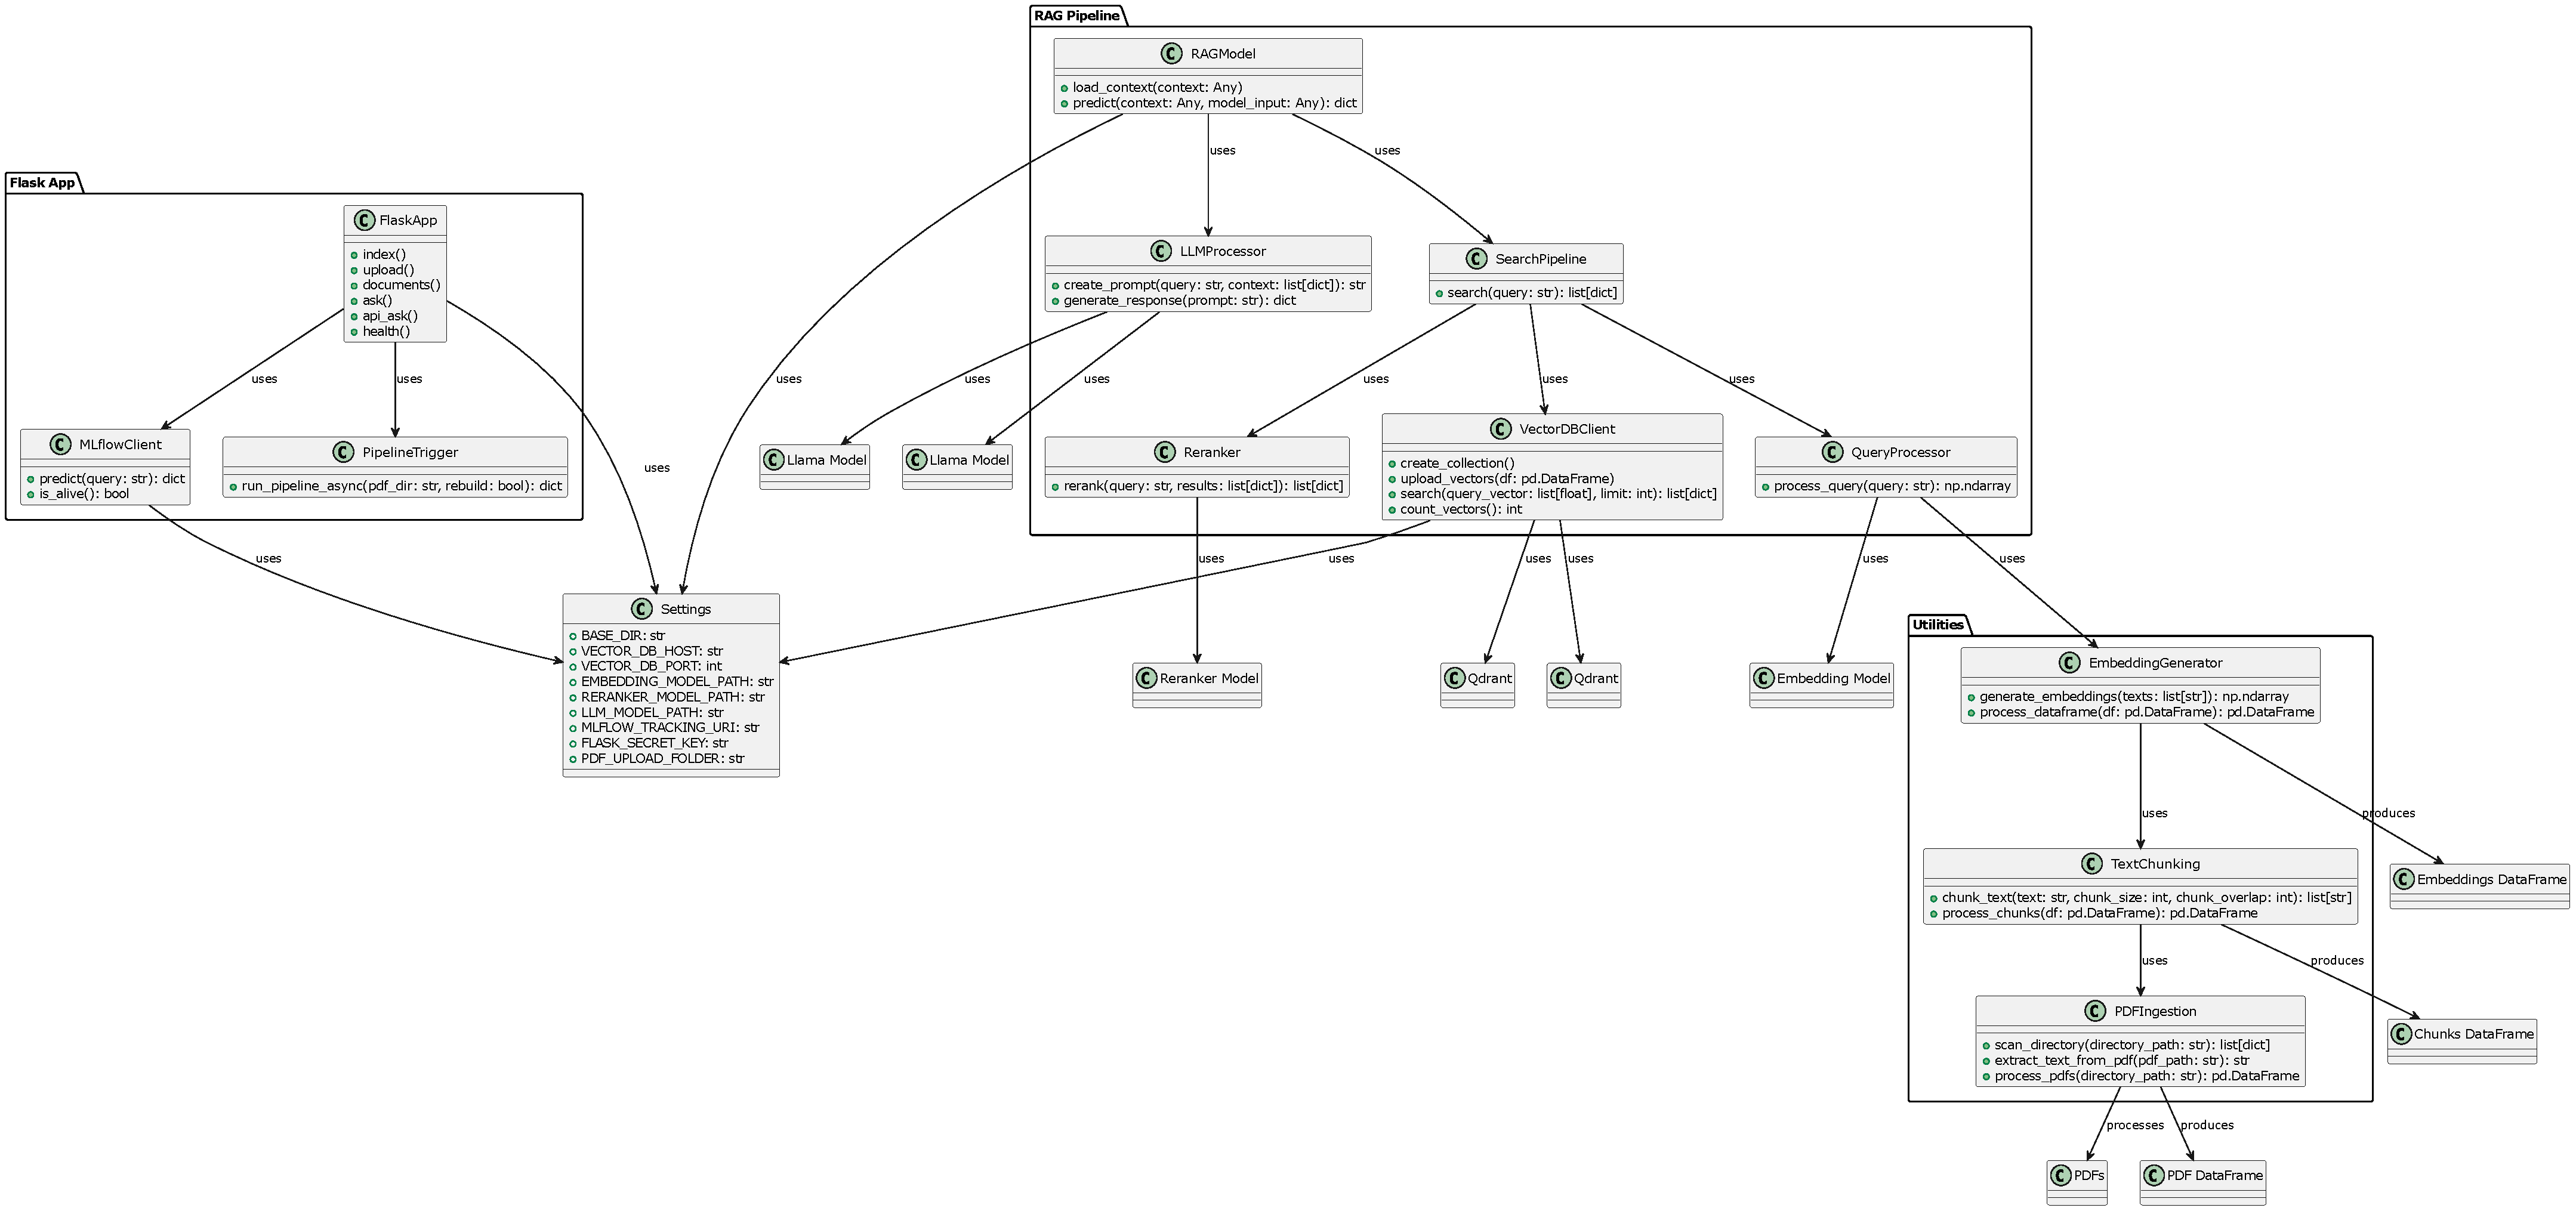
\includegraphics[keepaspectratio]{docs/puml/svg/class.pdf}}
\caption{Class Diagram}
\end{figure}

\subsubsection{Use Case Diagram}\label{use-case-diagram}

The use case diagram is shown below:

\begin{figure}
\centering
\pandocbounded{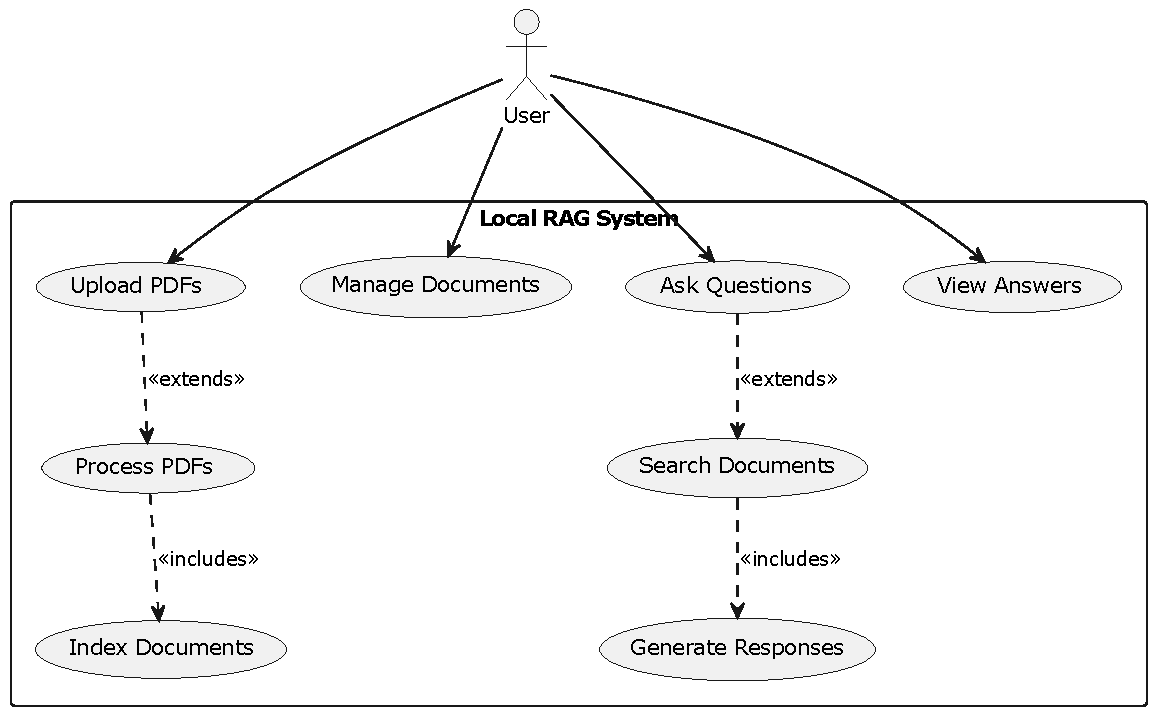
\includegraphics[keepaspectratio]{docs/puml/svg/usecase.pdf}}
\caption{Use Case Diagram}
\end{figure}

\subsubsection{Component Diagram}\label{component-diagram}

The component diagram is shown below:

\begin{figure}
\centering
\pandocbounded{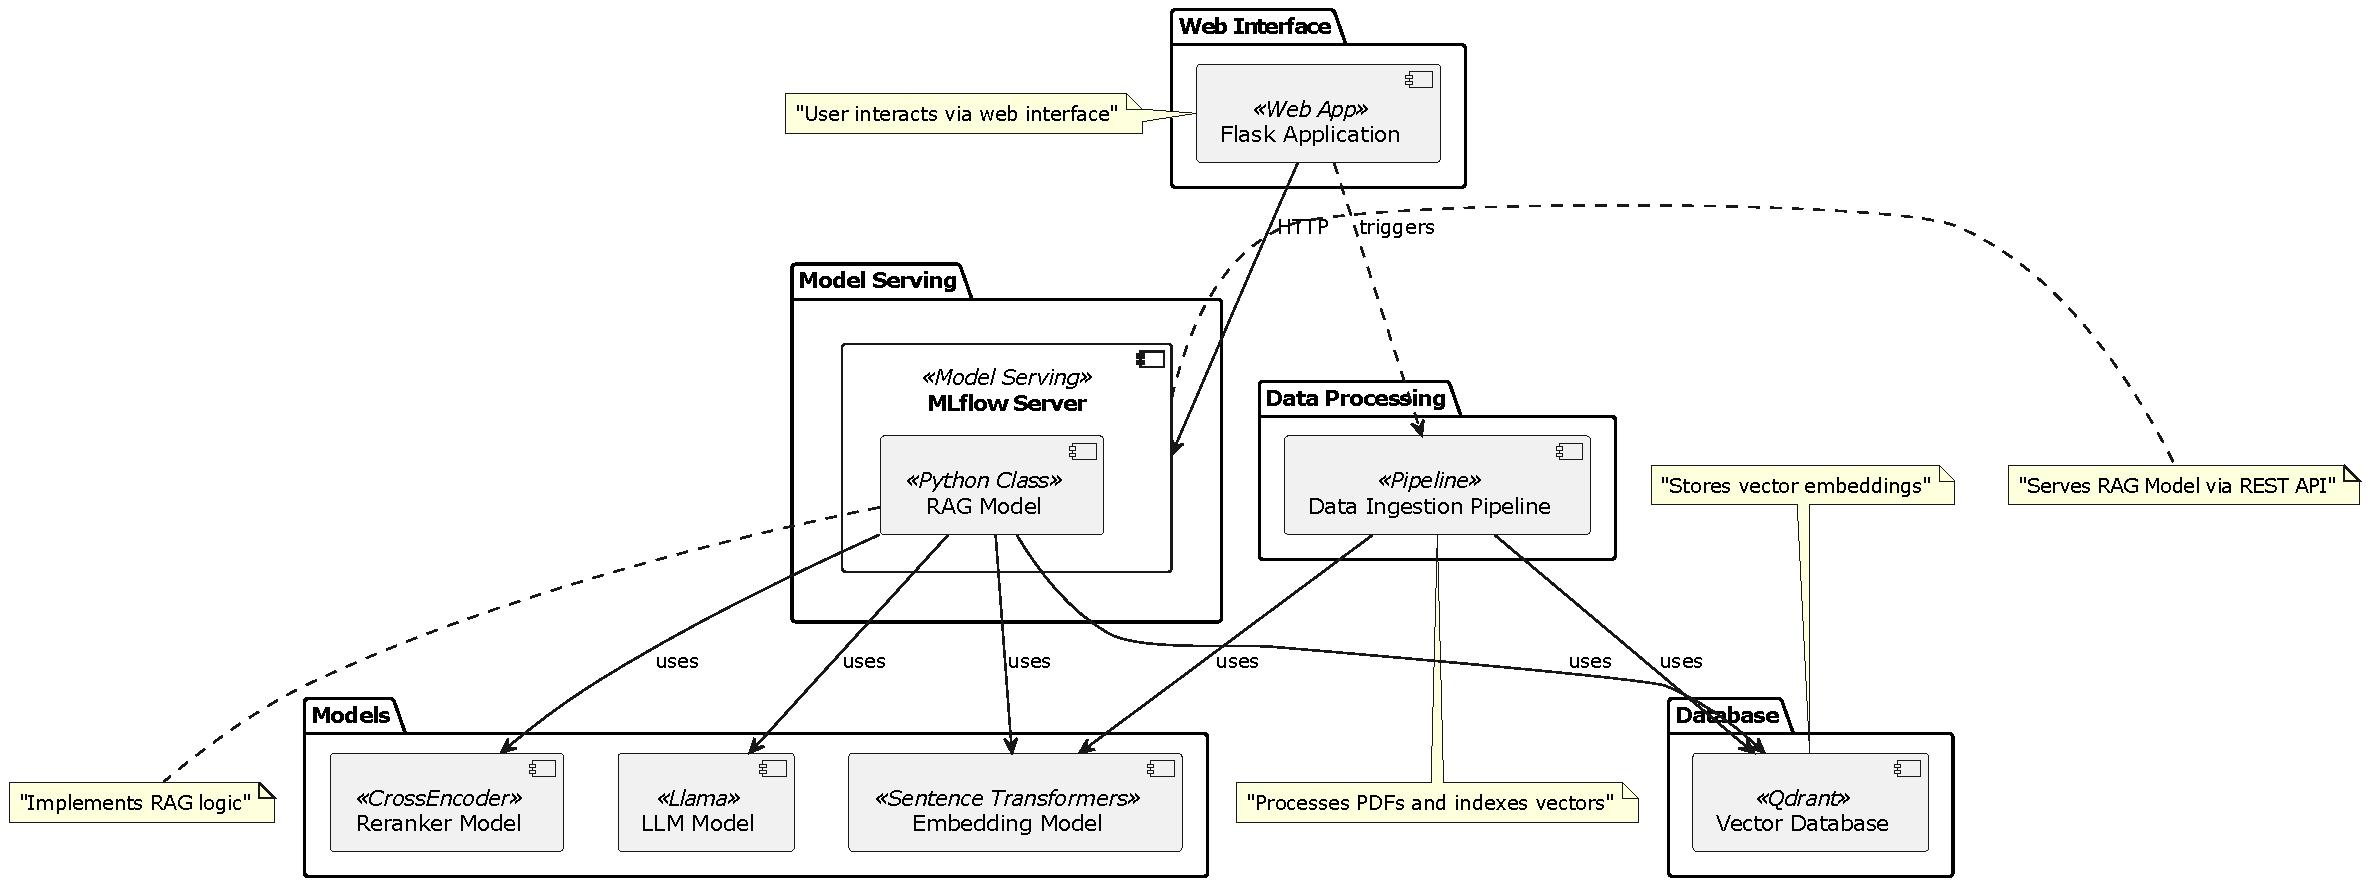
\includegraphics[keepaspectratio]{docs/puml/svg/component.pdf}}
\caption{Component Diagram}
\end{figure}

\subsubsection{Deployment Diagram}\label{deployment-diagram}

The deployment diagram is shown below:

\begin{figure}
\centering
\pandocbounded{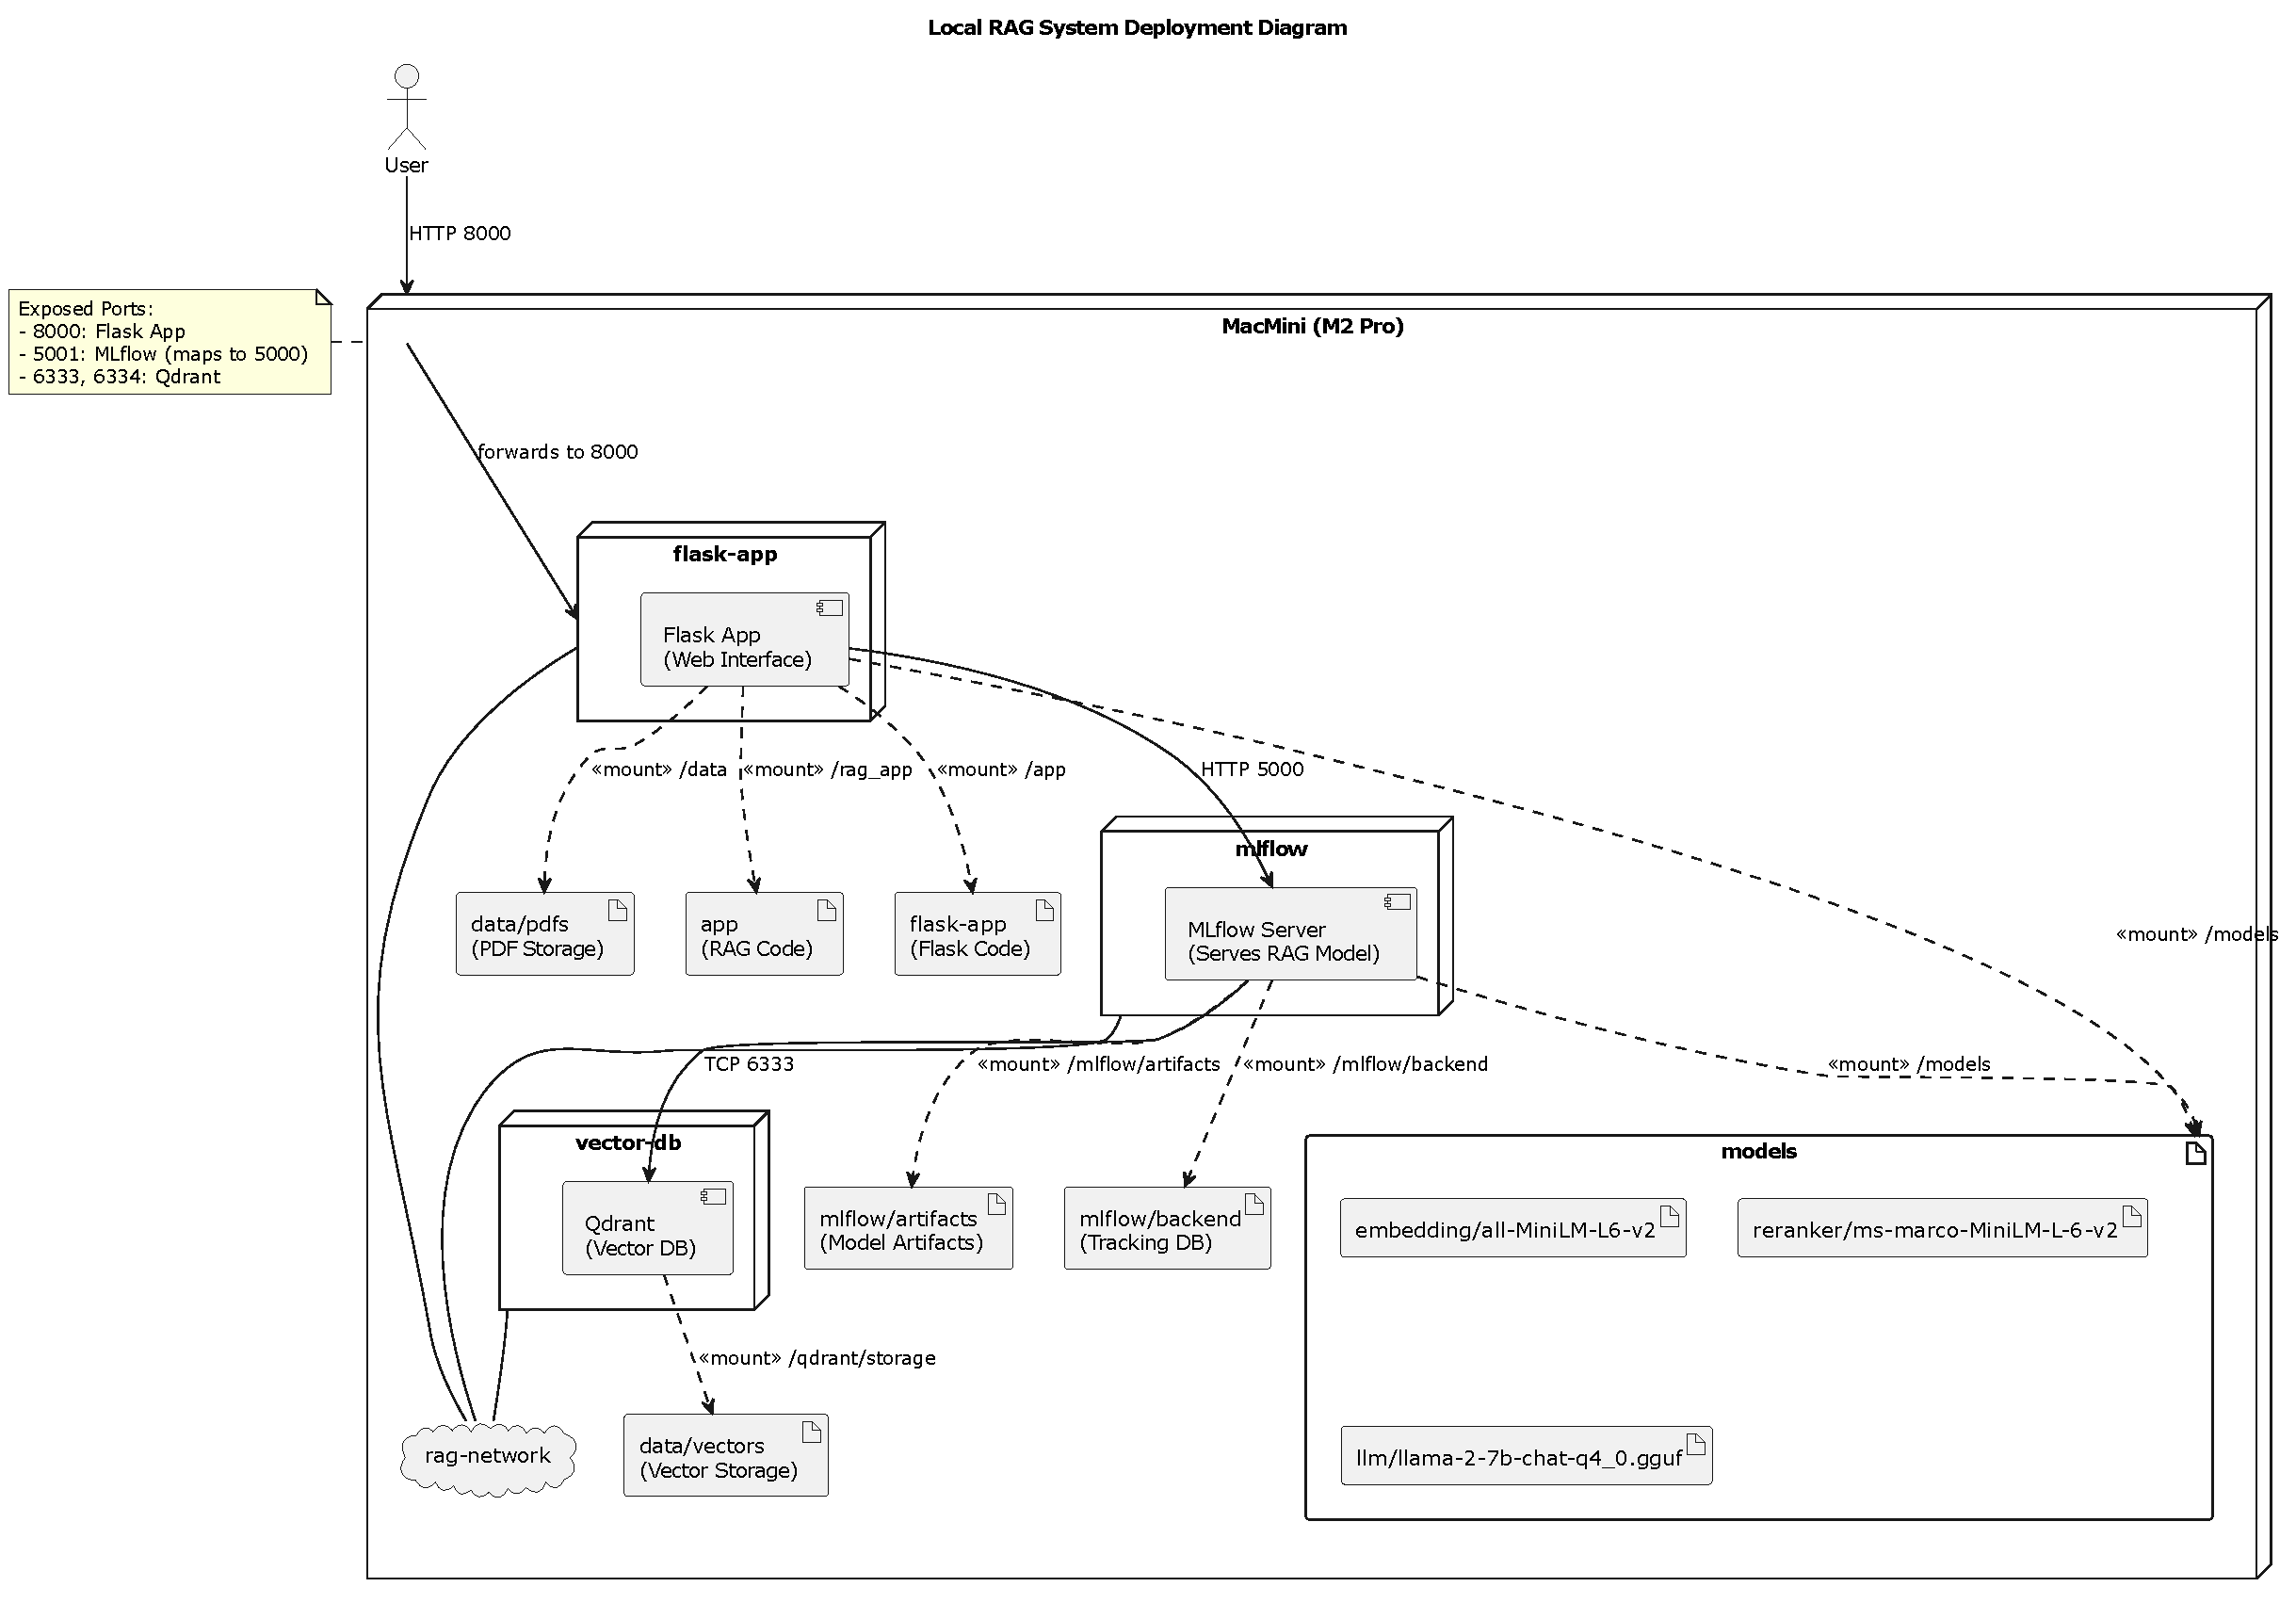
\includegraphics[keepaspectratio]{docs/puml/svg/deployment.pdf}}
\caption{Deployment Diagram}
\end{figure}

The is it for now :).

\end{document}
